\documentclass[]{book}
\usepackage{lmodern}
\usepackage{amssymb,amsmath}
\usepackage{ifxetex,ifluatex}
\usepackage{fixltx2e} % provides \textsubscript
\ifnum 0\ifxetex 1\fi\ifluatex 1\fi=0 % if pdftex
  \usepackage[T1]{fontenc}
  \usepackage[utf8]{inputenc}
\else % if luatex or xelatex
  \ifxetex
    \usepackage{mathspec}
  \else
    \usepackage{fontspec}
  \fi
  \defaultfontfeatures{Ligatures=TeX,Scale=MatchLowercase}
\fi
% use upquote if available, for straight quotes in verbatim environments
\IfFileExists{upquote.sty}{\usepackage{upquote}}{}
% use microtype if available
\IfFileExists{microtype.sty}{%
\usepackage[]{microtype}
\UseMicrotypeSet[protrusion]{basicmath} % disable protrusion for tt fonts
}{}
\PassOptionsToPackage{hyphens}{url} % url is loaded by hyperref
\usepackage[unicode=true]{hyperref}
\hypersetup{
            pdftitle={2020-01-15-brynmawr},
            pdfauthor={Kelsey Gonzalez, Amelia McNamara, The Carpentries},
            pdfborder={0 0 0},
            breaklinks=true}
\urlstyle{same}  % don't use monospace font for urls
\usepackage{natbib}
\bibliographystyle{apalike}
\usepackage{color}
\usepackage{fancyvrb}
\newcommand{\VerbBar}{|}
\newcommand{\VERB}{\Verb[commandchars=\\\{\}]}
\DefineVerbatimEnvironment{Highlighting}{Verbatim}{commandchars=\\\{\}}
% Add ',fontsize=\small' for more characters per line
\usepackage{framed}
\definecolor{shadecolor}{RGB}{248,248,248}
\newenvironment{Shaded}{\begin{snugshade}}{\end{snugshade}}
\newcommand{\KeywordTok}[1]{\textcolor[rgb]{0.13,0.29,0.53}{\textbf{#1}}}
\newcommand{\DataTypeTok}[1]{\textcolor[rgb]{0.13,0.29,0.53}{#1}}
\newcommand{\DecValTok}[1]{\textcolor[rgb]{0.00,0.00,0.81}{#1}}
\newcommand{\BaseNTok}[1]{\textcolor[rgb]{0.00,0.00,0.81}{#1}}
\newcommand{\FloatTok}[1]{\textcolor[rgb]{0.00,0.00,0.81}{#1}}
\newcommand{\ConstantTok}[1]{\textcolor[rgb]{0.00,0.00,0.00}{#1}}
\newcommand{\CharTok}[1]{\textcolor[rgb]{0.31,0.60,0.02}{#1}}
\newcommand{\SpecialCharTok}[1]{\textcolor[rgb]{0.00,0.00,0.00}{#1}}
\newcommand{\StringTok}[1]{\textcolor[rgb]{0.31,0.60,0.02}{#1}}
\newcommand{\VerbatimStringTok}[1]{\textcolor[rgb]{0.31,0.60,0.02}{#1}}
\newcommand{\SpecialStringTok}[1]{\textcolor[rgb]{0.31,0.60,0.02}{#1}}
\newcommand{\ImportTok}[1]{#1}
\newcommand{\CommentTok}[1]{\textcolor[rgb]{0.56,0.35,0.01}{\textit{#1}}}
\newcommand{\DocumentationTok}[1]{\textcolor[rgb]{0.56,0.35,0.01}{\textbf{\textit{#1}}}}
\newcommand{\AnnotationTok}[1]{\textcolor[rgb]{0.56,0.35,0.01}{\textbf{\textit{#1}}}}
\newcommand{\CommentVarTok}[1]{\textcolor[rgb]{0.56,0.35,0.01}{\textbf{\textit{#1}}}}
\newcommand{\OtherTok}[1]{\textcolor[rgb]{0.56,0.35,0.01}{#1}}
\newcommand{\FunctionTok}[1]{\textcolor[rgb]{0.00,0.00,0.00}{#1}}
\newcommand{\VariableTok}[1]{\textcolor[rgb]{0.00,0.00,0.00}{#1}}
\newcommand{\ControlFlowTok}[1]{\textcolor[rgb]{0.13,0.29,0.53}{\textbf{#1}}}
\newcommand{\OperatorTok}[1]{\textcolor[rgb]{0.81,0.36,0.00}{\textbf{#1}}}
\newcommand{\BuiltInTok}[1]{#1}
\newcommand{\ExtensionTok}[1]{#1}
\newcommand{\PreprocessorTok}[1]{\textcolor[rgb]{0.56,0.35,0.01}{\textit{#1}}}
\newcommand{\AttributeTok}[1]{\textcolor[rgb]{0.77,0.63,0.00}{#1}}
\newcommand{\RegionMarkerTok}[1]{#1}
\newcommand{\InformationTok}[1]{\textcolor[rgb]{0.56,0.35,0.01}{\textbf{\textit{#1}}}}
\newcommand{\WarningTok}[1]{\textcolor[rgb]{0.56,0.35,0.01}{\textbf{\textit{#1}}}}
\newcommand{\AlertTok}[1]{\textcolor[rgb]{0.94,0.16,0.16}{#1}}
\newcommand{\ErrorTok}[1]{\textcolor[rgb]{0.64,0.00,0.00}{\textbf{#1}}}
\newcommand{\NormalTok}[1]{#1}
\usepackage{longtable,booktabs}
% Fix footnotes in tables (requires footnote package)
\IfFileExists{footnote.sty}{\usepackage{footnote}\makesavenoteenv{long table}}{}
\usepackage{graphicx,grffile}
\makeatletter
\def\maxwidth{\ifdim\Gin@nat@width>\linewidth\linewidth\else\Gin@nat@width\fi}
\def\maxheight{\ifdim\Gin@nat@height>\textheight\textheight\else\Gin@nat@height\fi}
\makeatother
% Scale images if necessary, so that they will not overflow the page
% margins by default, and it is still possible to overwrite the defaults
% using explicit options in \includegraphics[width, height, ...]{}
\setkeys{Gin}{width=\maxwidth,height=\maxheight,keepaspectratio}
\IfFileExists{parskip.sty}{%
\usepackage{parskip}
}{% else
\setlength{\parindent}{0pt}
\setlength{\parskip}{6pt plus 2pt minus 1pt}
}
\setlength{\emergencystretch}{3em}  % prevent overfull lines
\providecommand{\tightlist}{%
  \setlength{\itemsep}{0pt}\setlength{\parskip}{0pt}}
\setcounter{secnumdepth}{5}
% Redefines (sub)paragraphs to behave more like sections
\ifx\paragraph\undefined\else
\let\oldparagraph\paragraph
\renewcommand{\paragraph}[1]{\oldparagraph{#1}\mbox{}}
\fi
\ifx\subparagraph\undefined\else
\let\oldsubparagraph\subparagraph
\renewcommand{\subparagraph}[1]{\oldsubparagraph{#1}\mbox{}}
\fi

% set default figure placement to htbp
\makeatletter
\def\fps@figure{htbp}
\makeatother

\usepackage{booktabs}
\usepackage{amsthm}
\makeatletter
\def\thm@space@setup{%
  \thm@preskip=8pt plus 2pt minus 4pt
  \thm@postskip=\thm@preskip
}
\makeatother

\title{2020-01-15-brynmawr}
\author{Kelsey Gonzalez, Amelia McNamara, The Carpentries}
\date{2020-01-13}

\begin{document}
\maketitle

{
\setcounter{tocdepth}{1}
\tableofcontents
}
\chapter*{Preface}\label{preface}
\addcontentsline{toc}{chapter}{Preface}

\section{General Information}\label{general-information}

Data Carpentry develops and teaches workshops on the fundamental data
skills needed to conduct research. Its target audience is researchers
who have little to no prior computational experience, and its lessons
are domain specific, building on learners' existing knowledge to enable
them to quickly apply skills learned to their own research. Participants
will be encouraged to help one another and to apply what they have
learned to their own research problems.

For more information on what we teach and why, please see our paper
\href{https://journals.plos.org/ploscompbiol/article?id=10.1371/journal.pcbi.1005510}{``Good
Enough Practices for Scientific Computing''}.

\textbf{Who}: The course is aimed at undergraduate students and other
researchers. You don't need to have any previous knowledge of the tools
that will be presented at the workshop.

\textbf{Where}: Park Science Center Rm 243. Get directions with
OpenStreetMap or Google Maps. Additionally, it is building \#13 on this
map.

\textbf{When}: Jan 15-16, 2020. Add to your Google Calendar.

\textbf{Requirements}: Participants must bring a laptop with a Mac,
Linux, or Windows operating system (not a tablet, Chromebook, etc.) that
they have administrative privileges on. They should have a few specific
software packages installed
(\href{https://datacarpentry.org/r-socialsci/setup.html}{R and
RStudio}).

Code of Conduct: Everyone who participates in Carpentries activities is
required to conform to the Code of Conduct. This document also outlines
how to report an incident if needed.

Contact: Please email
\href{mailto:jholling@brynmawr.edu}{\nolinkurl{jholling@brynmawr.edu}} ,
\href{mailto:amelia.mcnamara@stthomas.edu}{\nolinkurl{amelia.mcnamara@stthomas.edu}}
or
\href{mailto:kelseygonzalez@email.arizona.edu}{\nolinkurl{kelseygonzalez@email.arizona.edu}}
for more information.

\chapter{Introduction}\label{intro}

teaching: 25\\
exercises: 15\\
adapted from:
\url{https://datacarpentry.org/r-socialsci/00-intro/index.html}\\
\&
\url{http://swcarpentry.github.io/r-novice-gapminder/02-project-intro/index.html}

questions:

\begin{itemize}
\tightlist
\item
  How to find your way around RStudio?\\
\item
  How to interact with R?
\end{itemize}

objectives:

\begin{itemize}
\tightlist
\item
  Install latest version of R.\\
\item
  Install latest version of RStudio.\\
\item
  Navigate the RStudio GUI.
\item
  Create self-contained projects in RStudio
\end{itemize}

keypoints:

\begin{itemize}
\tightlist
\item
  Use RStudio to write and run R programs.
\end{itemize}

\section{What is R? What is RStudio?}\label{what-is-r-what-is-rstudio}

The term ``\texttt{R}'' is used to refer to both the programming
language and the software that interprets the scripts written using it.

\href{https://rstudio.com}{RStudio} is currently a very popular way to
not only write your R scripts but also to interact with the R software.
To function correctly, RStudio needs R and therefore both need to be
installed on your computer.

To make it easier to interact with R, we will use RStudio. RStudio is
the most popular IDE (Integrated Development Interface) for R. An IDE is
a piece of software that provides tools to make programming easier.

\section{Why learn R?}\label{why-learn-r}

\subsection{R does not involve lots of pointing and clicking, and that's
a good
thing}\label{r-does-not-involve-lots-of-pointing-and-clicking-and-thats-a-good-thing}

The learning curve might be steeper than with other software, but with
R, the results of your analysis do not rely on remembering a succession
of pointing and clicking, but instead on a series of written commands,
and that's a good thing! So, if you want to redo your analysis because
you collected more data, you don't have to remember which button you
clicked in which order to obtain your results; you just have to run your
script again.

Working with scripts makes the steps you used in your analysis clear,
and the code you write can be inspected by someone else who can give you
feedback and spot mistakes.

Working with scripts forces you to have a deeper understanding of what
you are doing, and facilitates your learning and comprehension of the
methods you use.

\subsection{R code is great for
reproducibility}\label{r-code-is-great-for-reproducibility}

Reproducibility is when someone else (including your future self) can
obtain the same results from the same dataset when using the same
analysis.

R integrates with other tools to generate manuscripts from your code. If
you collect more data, or fix a mistake in your dataset, the figures and
the statistical tests in your manuscript are updated automatically.

An increasing number of journals and funding agencies expect analyses to
be reproducible, so knowing R will give you an edge with these
requirements.

\subsection{R is interdisciplinary and
extensible}\label{r-is-interdisciplinary-and-extensible}

With 10,000+ packages that can be installed to extend its capabilities,
R provides a framework that allows you to combine statistical approaches
from many scientific disciplines to best suit the analytical framework
you need to analyze your data. For instance, R has packages for image
analysis, GIS, time series, population genetics, and a lot more.

\subsection{R works on data of all shapes and
sizes}\label{r-works-on-data-of-all-shapes-and-sizes}

The skills you learn with R scale easily with the size of your dataset.
Whether your dataset has hundreds or millions of lines, it won't make
much difference to you.

R is designed for data analysis. It comes with special data structures
and data types that make handling of missing data and statistical
factors convenient.

R can connect to spreadsheets, databases, and many other data formats,
on your computer or on the web.

\subsection{R produces high-quality
graphics}\label{r-produces-high-quality-graphics}

The plotting functionalities in R are endless, and allow you to adjust
any aspect of your graph to convey most effectively the message from
your data.

\subsection{R has a large and welcoming
community}\label{r-has-a-large-and-welcoming-community}

Thousands of people use R daily. Many of them are willing to help you
through mailing lists and websites such as
\href{https://stackoverflow.com/}{Stack Overflow}, or on the
\href{https://community.rstudio.com/}{RStudio community}. Questions
which are backed up with \href{https://www.tidyverse.org/help/}{short,
reproducible code snippets} are more likely to attract knowledgeable
responses.

\subsection{Not only is R free, but it is also open-source and
cross-platform}\label{not-only-is-r-free-but-it-is-also-open-source-and-cross-platform}

Anyone can inspect the source code to see how R works. Because of this
transparency, there is less chance for mistakes, and if you (or someone
else) find some, you can report and fix bugs.

Because R is open source and is supported by a large community of
developers and users, there is a very large selection of third-party
add-on packages which are freely available to extend R's native
capabilities.


\includegraphics{./fig/r+rstudio-analogy.jpg} RStudio extends what R can
do, and makes it easier to write R code and interact with R

\section{Knowing your way around
RStudio}\label{knowing-your-way-around-rstudio}

Let's start by learning about \href{https://www.rstudio.com/}{RStudio},
which is an Integrated Development Environment (IDE) for working with R.

The RStudio IDE open-source product is free under the
\href{https://www.gnu.org/licenses/agpl-3.0.en.html}{Affero General
Public License (AGPL) v3}. The RStudio IDE is also available with a
commercial license and priority email support from RStudio, Inc.

We will use the RStudio IDE to write code, navigate the files on our
computer, inspect the variables we create, and visualize the plots we
generate. RStudio can also be used for other things (e.g., version
control, developing packages, writing Shiny apps) that we will not cover
during the workshop.

One of the advantages of using RStudio is that all the information you
need to write code is available in a single window. Additionally,
RStudio provides many shortcuts, autocompletion, and highlighting for
the major file types you use while developing in R. RStudio makes typing
easier and less error-prone.

\section{Getting set up}\label{getting-set-up}

The scientific process is naturally incremental, and many projects start
life as random notes, some code, then a manuscript, and eventually
everything is a bit mixed together.

Most people tend to organize their projects like this:
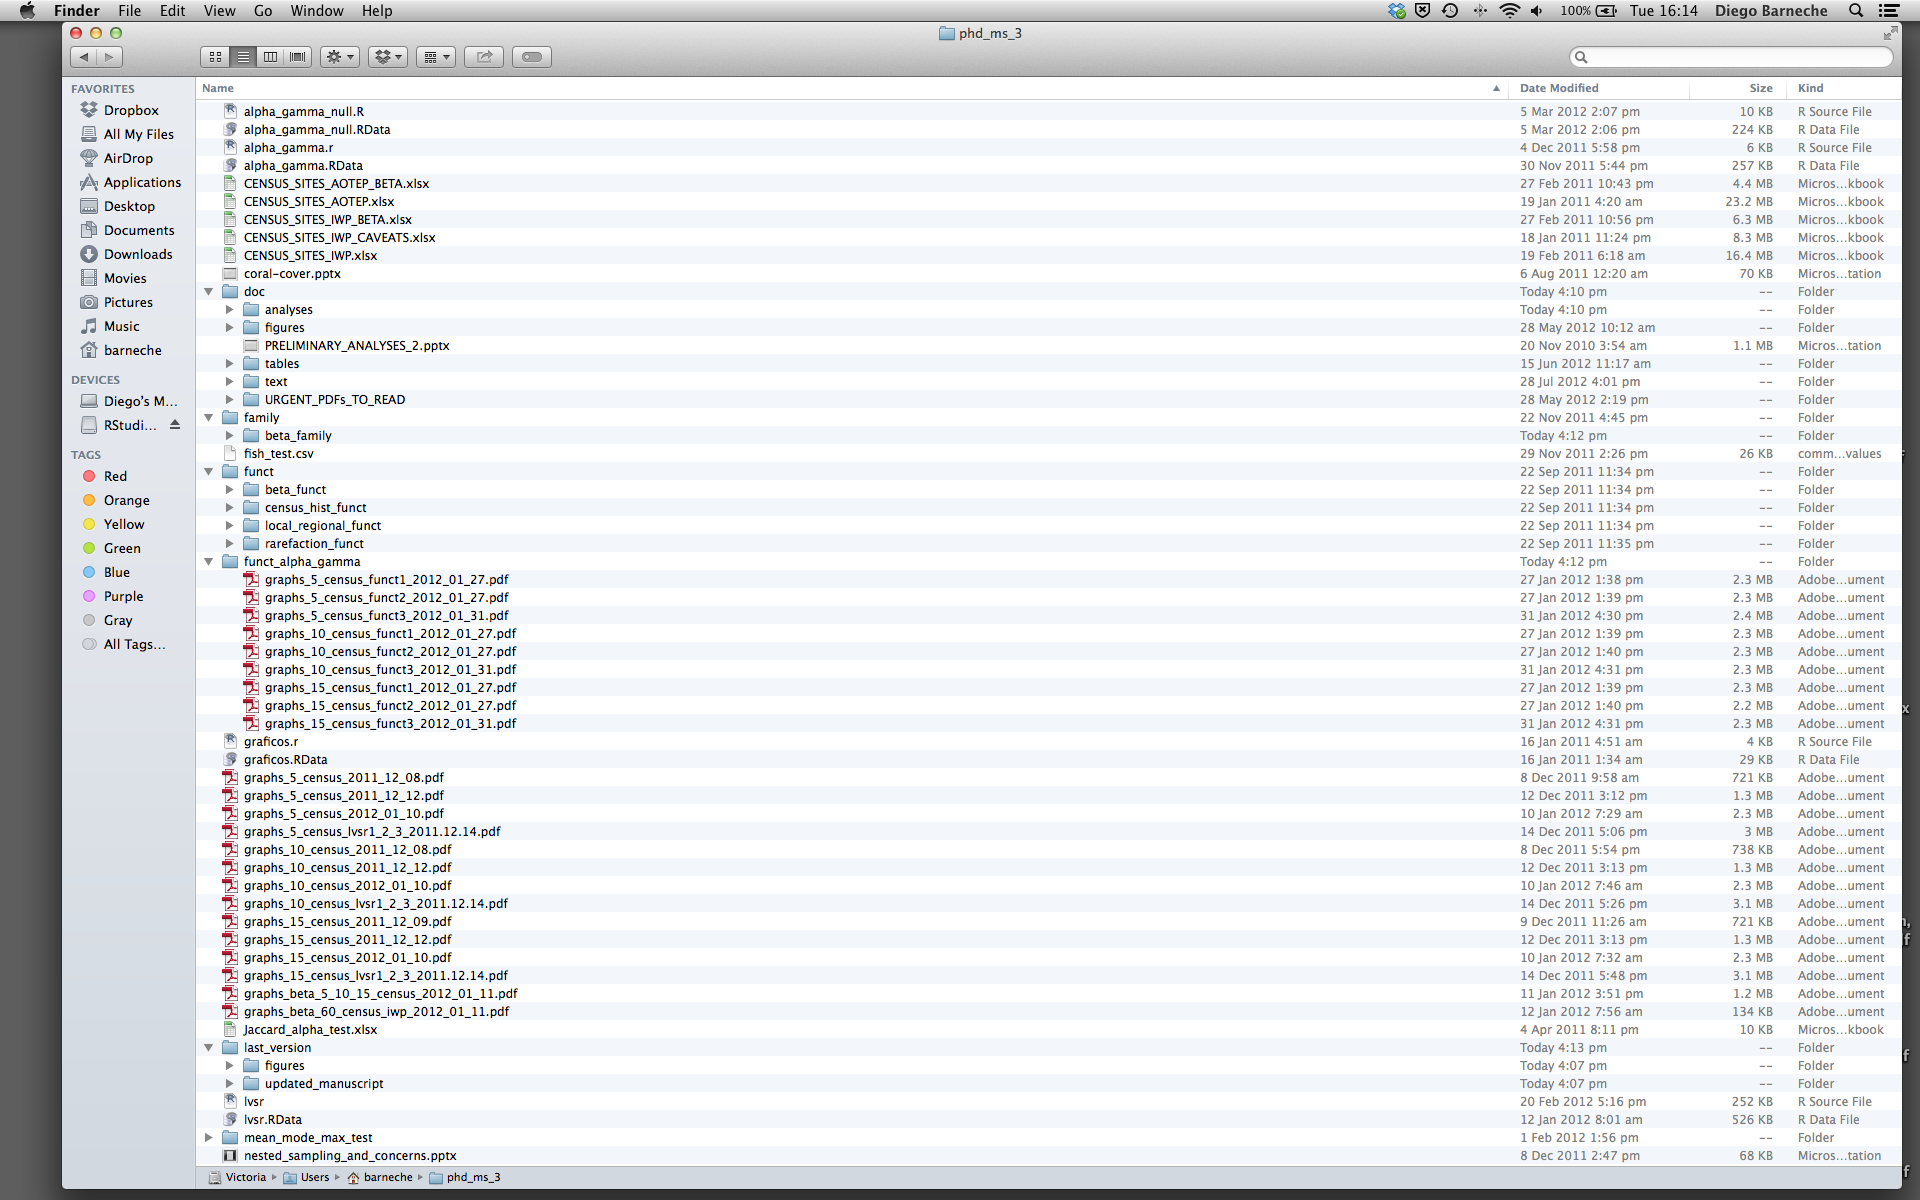
\includegraphics{./fig/bad_layout.png}

There are many reasons why we should \emph{ALWAYS} avoid this:

\begin{enumerate}
\def\labelenumi{\arabic{enumi}.}
\tightlist
\item
  It is really hard to tell which version of your data is the original
  and which is the modified;
\item
  It gets really messy because it mixes files with various extensions
  together;
\item
  It probably takes you a lot of time to actually find things, and
  relate the correct figures to the exact code that has been used to
  generate it;
\end{enumerate}

A good project layout will ultimately make your life easier:

\begin{itemize}
\tightlist
\item
  It will help ensure the integrity of your data;
\item
  It makes it simpler to share your code with someone else (a lab-mate,
  collaborator, or supervisor);
\item
  It allows you to easily upload your code with your manuscript
  submission;
\item
  It makes it easier to pick the project back up after a break.
\end{itemize}

It is good practice to keep a set of related data, analyses, and text
self-contained in a single folder called the \textbf{working directory}.
All of the scripts within this folder can then use \emph{relative paths}
to files. Relative paths indicate where inside the project a file is
located (as opposed to absolute paths, which point to where a file is on
a specific computer). Working this way makes it a lot easier to move
your project around on your computer and share it with others without
having to directly modify file paths in the individual scripts.

RStudio provides a helpful set of tools to do this through its
``Projects'' interface, which not only creates a working directory for
you but also remembers its location (allowing you to quickly navigate to
it). The interface also (optionally) preserves custom settings and open
files to make it easier to resume work after a break.

\subsection{Create a new project}\label{create-a-new-project}

\begin{itemize}
\tightlist
\item
  Under the \texttt{File} menu, click on \texttt{New\ project}, choose
  \texttt{New\ directory}, then \texttt{New\ project}
\item
  Enter a name for this new folder (or ``directory'') and choose a
  convenient location for it. This will be your \textbf{working
  directory} for the rest of the day (e.g.,
  \texttt{\textasciitilde{}/data-carpentry})
\item
  Click on \texttt{Create\ project}
\item
  Create a new file where we will type our scripts. Go to File
  \textgreater{} New File \textgreater{} R script. Click the save icon
  on your toolbar and save your script as ``\texttt{script.R}''.
\end{itemize}

Now when we start R in this project directory, or open this project with
RStudio, all of our work on this project will be entirely self-contained
in this directory.

\subsection{The RStudio Interface}\label{the-rstudio-interface}

Let's take a quick tour of RStudio.
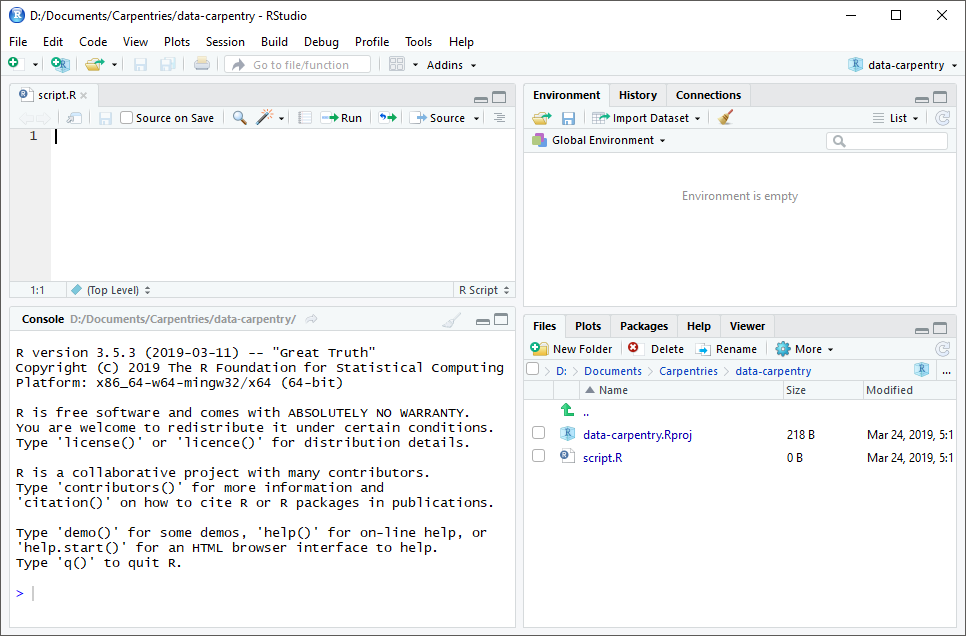
\includegraphics{./fig/R_00_Rstudio_01.png} RStudio is divided into four
``panes''. The placement of these panes and their content can be
customized (see menu, Tools -\textgreater{} Global Options
-\textgreater{} Pane Layout).

The Default Layout is: - Top Left - \textbf{Source}: your scripts and
documents - Bottom Left - \textbf{Console}: what R would look and be
like without RStudio - Top Right - \textbf{Enviornment/History}: look
here to see what you have done - Bottom Right - \textbf{Files} and more:
see the contents of the project/working directory here, like your
Script.R file

\subsection{Organizing your working
directory}\label{organizing-your-working-directory}

Using a consistent folder structure across your projects will help keep
things organized and make it easy to find/file things in the future.
This can be especially helpful when you have multiple projects. In
general, you might create directories (folders) for \textbf{scripts},
\textbf{data}, and \textbf{documents}. Here are some examples of
suggested directories:

\begin{itemize}
\tightlist
\item
  \textbf{\texttt{data/}} Use this folder to store your raw data and
  intermediate datasets. For the sake of transparency and
  \href{https://en.wikipedia.org/wiki/Provenance}{provenance}, you
  should \emph{always} keep a copy of your raw data accessible and do as
  much of your data cleanup and preprocessing programmatically (i.e.,
  with scripts, rather than manually) as possible.
\item
  \textbf{\texttt{data\_output/}} When you need to modify your raw data,
  it might be useful to store the modified versions of the datasets in a
  different folder.
\item
  \textbf{\texttt{documents/}} Used for outlines, drafts, and other
  text.
\item
  \textbf{\texttt{fig\_output/}} This folder can store the graphics that
  are generated by your scripts.
\item
  \textbf{\texttt{scripts/}} A place to keep your R scripts for
  different analyses or plotting.
\end{itemize}

You may want additional directories or subdirectories depending on your
project needs, but these should form the backbone of your working
directory.

\begin{figure}
\centering
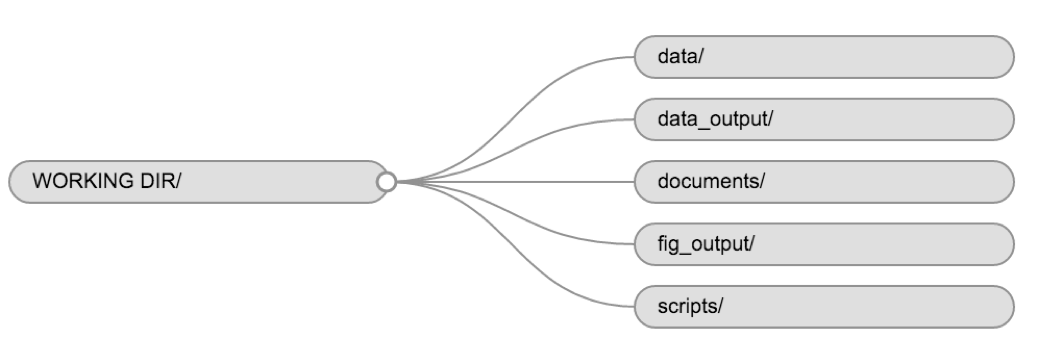
\includegraphics{./fig/working-directory-structure.png}
\caption{Example of a working directory structure}
\end{figure}

\subsection{The working directory}\label{the-working-directory}

The working directory is an important concept to understand. It is the
place where R will look for and save files. When you write code for your
project, your scripts should refer to files in relation to the root of
your working directory and only to files within this structure.

Using RStudio projects makes this easy and ensures that your working
directory is set up properly. If you need to check it, you can use
\texttt{getwd()}. If for some reason your working directory is not what
it should be, you can change it in the RStudio interface by navigating
in the file browser to where your working directory should be, clicking
on the blue gear icon ``More'', and selecting ``Set As Working
Directory''. Alternatively, you can use
\texttt{setwd("/path/to/working/directory")} to reset your working
directory. However, your scripts should not include this line, because
it will fail on someone else's computer.

\section{Interacting with R}\label{interacting-with-r}

The basis of programming is that we write down instructions for the
computer to follow, and then we tell the computer to follow those
instructions. We write, or \emph{code}, instructions in R because it is
a common language that both the computer and we can understand. We call
the instructions \emph{commands} and we tell the computer to follow the
instructions by \emph{executing} (also called \emph{running}) those
commands.

There are two main ways of interacting with R: by using the console or
by using script files (plain text files that contain your code). The
console pane (in RStudio, the bottom left panel) is the place where
commands written in the R language can be typed and executed immediately
by the computer. It is also where the results will be shown for commands
that have been executed. You can type commands directly into the console
and press Enter to execute those commands, but they will be forgotten
when you close the session.

Because we want our code and workflow to be reproducible, it is better
to type the commands we want in the script editor and save the script.
This way, there is a complete record of what we did, and anyone
(including our future selves!) can easily replicate the results on their
computer.

RStudio allows you to execute commands directly from the script editor
by using the Ctrl + Enter shortcut (on Mac, Cmd + Return will work). The
command on the current line in the script (indicated by the cursor) or
all of the commands in selected text will be sent to the console and
executed when you press Ctrl + Enter. If there is information in the
console you do not need anymore, you can clear it with Ctrl + L.

You can find other keyboard shortcuts in this
\href{https://github.com/rstudio/cheatsheets/raw/master/rstudio-ide.pdf}{RStudio
cheatsheet about the RStudio IDE}.

At some point in your analysis, you may want to check the content of a
variable or the structure of an object without necessarily keeping a
record of it in your script. You can type these commands and execute
them directly in the console. RStudio provides the Ctrl + 1 and Ctrl + 2
shortcuts allow you to jump between the script and the console panes.

If R is ready to accept commands, the R console shows a
\texttt{\textgreater{}} prompt. If R receives a command (by typing,
copy-pasting, or sent from the script editor using Ctrl + Enter), R will
try to execute it and, when ready, will show the results and come back
with a new \texttt{\textgreater{}} prompt to wait for new commands.

If R is still waiting for you to enter more text, the console will show
a \texttt{+} prompt. It means that you haven't finished entering a
complete command. This is likely because you have not `closed' a
parenthesis or quotation, i.e.~you don't have the same number of
left-parentheses as right-parentheses or the same number of opening and
closing quotation marks.

When this happens, and you thought you finished typing your command,
click inside the console window and press Esc; this will cancel the
incomplete command and return you to the \texttt{\textgreater{}} prompt.
You can then proofread the command(s) you entered and correct the error.

\chapter{Getting Our Project Organized}\label{projectmanagement}

teaching: 20\\
exercises: 10\\
adapted from:
\url{http://swcarpentry.github.io/r-novice-gapminder/02-project-intro/index.html}

questions:

\begin{itemize}
\tightlist
\item
  How do I actually begin coding in R?
\item
  How to manage your environment?\\
\item
  How to install packages?
\end{itemize}

objectives:

\begin{itemize}
\tightlist
\item
  Organize our new package directory
\item
  Install additional packages using \texttt{install.packages()} command
\item
  Create our first rmarkdown document
\end{itemize}

keypoints:

\begin{itemize}
\tightlist
\item
  Use RStudio to create and manage projects with consistent layout.\\
\item
  Use \texttt{install.packages()} to install packages (libraries).
\end{itemize}

\subsection{Downloading the data and getting set
up}\label{downloading-the-data-and-getting-set-up}

For this lesson we will use the following folders in our working
directory: \textbf{\texttt{data/}}, \textbf{\texttt{data\_output/}} and
\textbf{\texttt{fig\_output/}}. Let's write them all in lowercase to be
consistent. We can create them using the RStudio interface by clicking
on the ``New Folder'' button in the file pane (bottom right), or
directly from R by typing at console:

\begin{Shaded}
\begin{Highlighting}[]
\KeywordTok{dir.create}\NormalTok{(}\StringTok{"data"}\NormalTok{)}
\KeywordTok{dir.create}\NormalTok{(}\StringTok{"data_output"}\NormalTok{)}
\KeywordTok{dir.create}\NormalTok{(}\StringTok{"fig_output"}\NormalTok{)}
\end{Highlighting}
\end{Shaded}

\section{Installing packages using the packages
command}\label{installing-packages-using-the-packages-command}

In addition to the core R installation, there are in excess of 10,000
additional packages which can be used to extend the functionality of R.
Many of these have been written by R users and have been made available
in central repositories, like the one hosted at CRAN, for anyone to
download and install into their own R environment. In the course of this
lesson we will be making use of several of these packages, such as
`ggplot2' and `dplyr'.

Additional packages can be installed from the command line or within a
script.

\begin{quote}
\section{Exercise}\label{exercise}

Use the console to install the tidyverse package. Find the console
(bottom left pane) and type

\begin{verbatim}
install.packages("tidyverse")
\end{verbatim}

The `tidyverse' package is really a package of packages, including
`ggplot2' and `dplyr', both of which require other packages to run
correctly. All of these packages will be installed automatically.
Depending on what packages have previously been installed in your R
environment, the install of `tidyverse' could be very quick or could
take several minutes. As the install proceeds, messages relating to its
progress will be written to the console. You will be able to see all of
the packages which are actually being installed.
\end{quote}

Because the install process accesses the CRAN repository, you will need
an Internet connection to install packages.

It is also possible to install packages from other repositories, as well
as Github or the local file system, but we won't be looking at these
options in this lesson.

We will also need a package called knitr. \textgreater{}
\texttt{\textgreater{}\ install.packages("tidyverse")\ \textgreater{}}
\textgreater{} As the install proceeds, messages relating to its
progress will be written to the console. You will be able to see all of
the packages which are actually being installed.

\section{Creating an R Markdown file}\label{creating-an-r-markdown-file}

Within RStudio, click File → New File → R Markdown and you'll get a
dialog box like this: 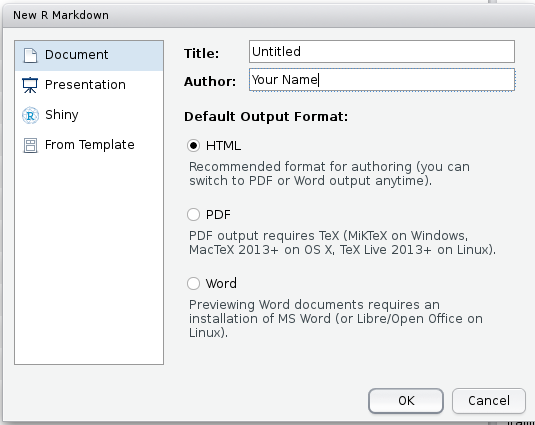
\includegraphics{./fig/New_R_Markdown.png}

You can stick with the default (HTML output), but let's call it
``intro-to-r''.

\section{Basic components of R
Markdown}\label{basic-components-of-r-markdown}

The initial chunk of text (header) contains instructions for R to
specify what kind of document will be created, and the options chosen.
You can use the header to give your document a title, author, date, and
tell it that you're going to want to produce html output (in other
words, a web page).

\begin{verbatim}
---
title: "Initial R Markdown document"
author: "Karl Broman"
date: "April 23, 2015"
output: html_document
---
\end{verbatim}

You can delete any of those fields if you don't want them included. The
double-quotes aren't strictly \emph{necessary} in this case. They're
mostly needed if you want to include a colon in the title.

RStudio creates the document with some example text to get you started.
Note below that there are chunks like

These are chunks of R code that will be executed by \texttt{knitr} and
replaced by their results. More on this later.

A quick preview of markdown formatting you can use before we delve in
deeper tomorrow:

to add headers of various sizes, use:

\begin{verbatim}
# Title
## Main section
### Sub-section
#### Sub-sub section
\end{verbatim}

You make things \textbf{bold} using two asterisks, like this:
\texttt{**bold**}, and you make things \emph{italics} by using
underscores, like this: \texttt{\_italics\_}.

Go ahead and write this down for reference as we learn today.

Next, we will download the dataset needed for these lessons. We won't be
using this right away, but we want to be prepared for when we need it.
I'll paste this into the etherpad, but we will be entering a command to
download a dataset from the internet to a specific destination.

\begin{Shaded}
\begin{Highlighting}[]
\KeywordTok{download.file}\NormalTok{(}\StringTok{"https://ndownloader.figshare.com/files/11492171"}\NormalTok{,}
              \StringTok{"data/SAFI_clean.csv"}\NormalTok{, }\DataTypeTok{mode =} \StringTok{"wb"}\NormalTok{)}
\end{Highlighting}
\end{Shaded}

Notice that this is being downloaded into our data folder. We can access
that destination from our current working directory by including the
data/ in front of the file name.

\chapter{Introduction to R}\label{basicR}

teaching: 50\\
exercises: 30\\
adapted from:
\url{https://datacarpentry.org/r-socialsci/01-intro-to-r/index.html}

questions:

\begin{itemize}
\tightlist
\item
  What data types are available in R?\\
\item
  What is an object?\\
\item
  How can values be initially assigned to variables of different data
  types?\\
\item
  What arithmetic and logical operators can be used?\\
\item
  How can subsets be extracted from vectors and data frames?\\
\item
  How does R treat missing values?\\
\item
  How can we deal with missing values in R?
\end{itemize}

objectives:

\begin{itemize}
\tightlist
\item
  Define the following terms as they relate to R: object, assign, call,
  function, arguments, options.\\
\item
  Assign values to objects in R.\\
\item
  Learn how to name objects.\\
\item
  Use comments to inform script.\\
\item
  Solve simple arithmetic operations in R.\\
\item
  Call functions and use arguments to change their default options.\\
\item
  Inspect the content of vectors and manipulate their content.\\
\item
  Subset and extract values from vectors.\\
\item
  Analyze vectors with missing data.
\end{itemize}

keypoints:

\begin{itemize}
\tightlist
\item
  Access individual values by location using \texttt{{[}{]}}.\\
\item
  Access arbitrary sets of data using \texttt{{[}c(...){]}}.\\
\item
  Use logical operations and logical vectors to access subsets of data.
\end{itemize}

\section{Creating objects in R}\label{creating-objects-in-r}

You can get output from R simply by typing math in the console:

\begin{Shaded}
\begin{Highlighting}[]
\DecValTok{3} \OperatorTok{+}\StringTok{ }\DecValTok{5}
\end{Highlighting}
\end{Shaded}

\begin{verbatim}
## [1] 8
\end{verbatim}

\begin{Shaded}
\begin{Highlighting}[]
\DecValTok{12} \OperatorTok{/}\StringTok{ }\DecValTok{7}
\end{Highlighting}
\end{Shaded}

\begin{verbatim}
## [1] 1.714286
\end{verbatim}

However, to do useful and interesting things, we need to assign
\emph{values} to \emph{objects}. To create an object, we need to give it
a name followed by the assignment operator \texttt{\textless{}-}, and
the value we want to give it:

\begin{Shaded}
\begin{Highlighting}[]
\NormalTok{area_hectares <-}\StringTok{ }\FloatTok{1.0}
\end{Highlighting}
\end{Shaded}

\texttt{\textless{}-} is the assignment operator. It assigns values on
the right to objects on the left. So, after executing
\texttt{x\ \textless{}-\ 3}, the value of \texttt{x} is \texttt{3}. The
arrow can be read as 3 \textbf{goes into} \texttt{x}. For historical
reasons, you can also use \texttt{=} for assignments. There are
\href{http://blog.revolutionanalytics.com/2008/12/use-equals-or-arrow-for-assignment.html}{slight}
\href{http://r.789695.n4.nabble.com/Is-there-any-difference-between-and-tp878594p878598.html}{differences}
depending on which syntax you use, and people have their own
preferences. Famous R programmer Yihui Xie
\href{https://yihui.org/en/2014/07/a-few-notes-on-user2014/}{insists on
=}, but many code style guides
\href{https://style.tidyverse.org/syntax.html\#assignment}{recommend
\textless{}-}. Use whichever one feels more comfortable to you!
(Typically, we recommend being consistent and just using one throughout
all your code.)

In RStudio, typing Alt + - (push Alt at the same time as the - key) will
write \texttt{\textless{}-} in a single keystroke in a PC, while typing
Option + - (push Option at the same time as the - key) does the same in
a Mac.

Objects can be given any name such as \texttt{x},
\texttt{current\_temperature}, or \texttt{subject\_id}. You want your
object names to be explicit and not too long. They cannot start with a
number (\texttt{2x} is not valid, but \texttt{x2} is). R is case
sensitive (e.g., \texttt{age} is different from \texttt{Age}). There are
some names that cannot be used because they are the names of fundamental
functions in R (e.g., \texttt{if}, \texttt{else}, \texttt{for}, see
\href{https://stat.ethz.ch/R-manual/R-devel/library/base/html/Reserved.html}{here}
for a complete list). In general, even if it's allowed, it's best to not
use other function names (e.g., \texttt{c}, \texttt{T}, \texttt{mean},
\texttt{data}, \texttt{df}, \texttt{weights}). If in doubt, check the
help to see if the name is already in use. It's also best to avoid dots
(\texttt{.}) within an object name as in \texttt{my.dataset}. There are
many functions in R with dots in their names for historical reasons, but
because dots have a special meaning in R (for methods) and other
programming languages, it's best to avoid them. It is also recommended
to use nouns for object names, and verbs for function names. It's
important to be consistent in the styling of your code (where you put
spaces, how you name objects, etc.). Using a consistent coding style
makes your code clearer to read for your future self and your
collaborators. In R, three popular style guides are
\href{https://google.github.io/styleguide/Rguide.xml}{Google's},
\href{http://jef.works/R-style-guide/}{Jean Fan's} and the
\href{http://style.tidyverse.org/}{tidyverse's}. The tidyverse's is very
comprehensive and may seem overwhelming at first. You can install the
\href{https://github.com/jimhester/lintr}{\textbf{\texttt{lintr}}}
package to automatically check for issues in the styling of your code.

\begin{quote}
\section{Objects vs.~variables}\label{objects-vs.variables}

What are known as \texttt{objects} in \texttt{R} are known as
\texttt{variables} in many other programming languages. Depending on the
context, \texttt{object} and \texttt{variable} can have drastically
different meanings. However, in this lesson, the two words are used
synonymously. For more information see:
\url{https://cran.r-project.org/doc/manuals/r-release/R-lang.html\#Objects}
\end{quote}

When assigning a value to an object, R does not print anything. You can
force R to print the value by using parentheses or by typing the object
name:

\begin{Shaded}
\begin{Highlighting}[]
\NormalTok{area_hectares <-}\StringTok{ }\FloatTok{1.0}    \CommentTok{# doesn't print anything}
\NormalTok{(area_hectares <-}\StringTok{ }\FloatTok{1.0}\NormalTok{)  }\CommentTok{# putting parenthesis around the call prints the value of `area_hectares`}
\end{Highlighting}
\end{Shaded}

\begin{verbatim}
## [1] 1
\end{verbatim}

\begin{Shaded}
\begin{Highlighting}[]
\NormalTok{area_hectares         }\CommentTok{# and so does typing the name of the object}
\end{Highlighting}
\end{Shaded}

\begin{verbatim}
## [1] 1
\end{verbatim}

Now that R has \texttt{area\_hectares} in memory, we can do arithmetic
with it. For instance, we may want to convert this area into acres (area
in acres is 2.47 times the area in hectares):

\begin{Shaded}
\begin{Highlighting}[]
\FloatTok{2.47} \OperatorTok{*}\StringTok{ }\NormalTok{area_hectares}
\end{Highlighting}
\end{Shaded}

\begin{verbatim}
## [1] 2.47
\end{verbatim}

We can also change an object's value by assigning it a new one:

\begin{Shaded}
\begin{Highlighting}[]
\NormalTok{area_hectares <-}\StringTok{ }\FloatTok{2.5}
\FloatTok{2.47} \OperatorTok{*}\StringTok{ }\NormalTok{area_hectares}
\end{Highlighting}
\end{Shaded}

\begin{verbatim}
## [1] 6.175
\end{verbatim}

This means that assigning a value to one object does not change the
values of other objects For example, let's store the plot's area in
acres in a new object, \texttt{area\_acres}:

\begin{Shaded}
\begin{Highlighting}[]
\NormalTok{area_acres <-}\StringTok{ }\FloatTok{2.47} \OperatorTok{*}\StringTok{ }\NormalTok{area_hectares}
\end{Highlighting}
\end{Shaded}

and then change \texttt{area\_hectares} to 50.

\begin{Shaded}
\begin{Highlighting}[]
\NormalTok{area_hectares <-}\StringTok{ }\DecValTok{50}
\end{Highlighting}
\end{Shaded}

\begin{quote}
\section{Exercise}\label{exercise-1}

What do you think is the current content of the object
\texttt{area\_acres}? 123.5 or 6.175? \textgreater{} \#\# Solution
\textgreater{} \textgreater{} The value of \texttt{area\_acres} is still
6.175 because you have not re-run the line
\texttt{area\_acres\ \textless{}-\ 2.47\ *\ area\_hectares} since
changing the value of \texttt{area\_hectares}.
\end{quote}

\section{Comments}\label{comments}

All programming languages allow the programmer to include comments in
their code. To do this in R we use the \texttt{\#} character. Anything
to the right of the \texttt{\#} sign and up to the end of the line is
treated as a comment and is ignored by R. You can start lines with
comments or include them after any code on the line.

\begin{Shaded}
\begin{Highlighting}[]
\NormalTok{area_hectares <-}\StringTok{ }\FloatTok{1.0}            \CommentTok{# land area in hectares}
\NormalTok{area_acres <-}\StringTok{ }\NormalTok{area_hectares }\OperatorTok{*}\StringTok{ }\FloatTok{2.47}  \CommentTok{# convert to acres}
\NormalTok{area_acres              }\CommentTok{# print land area in acres.}
\end{Highlighting}
\end{Shaded}

\begin{verbatim}
## [1] 2.47
\end{verbatim}

RStudio makes it easy to comment or uncomment a paragraph: after
selecting the lines you want to comment, press at the same time on your
keyboard Ctrl + Shift + C. If you only want to comment out one line, you
can put the cursor at any location of that line (i.e.~no need to select
the whole line), then press Ctrl + Shift + C.

\begin{quote}
\section{Exercise}\label{exercise-2}

Create two variables \texttt{my\_length} and \texttt{my\_width} and
assign them values. We will use these variable names rather than
\texttt{length} and \texttt{width} because \texttt{length} is already
function in R. If you use it as a variable name, RStudio might add
``()'' after length and if you leave the parentheses you will get
unexpected results. This is why you might see other programmers
abbreviate common words. Create a third variable \texttt{area} and give
it a value based on the current values of \texttt{my\_length} and
\texttt{my\_width}. Show that changing the values of either
\texttt{my\_length} and \texttt{my\_width} does not affect the value of
\texttt{area}.

\begin{quote}
\section{Solution}\label{solution}

\begin{Shaded}
\begin{Highlighting}[]
\NormalTok{my_length <-}\StringTok{ }\FloatTok{2.5}
\NormalTok{my_width <-}\StringTok{ }\FloatTok{3.2}
\NormalTok{area <-}\StringTok{ }\NormalTok{my_length }\OperatorTok{*}\StringTok{ }\NormalTok{my_width}
\NormalTok{area}
\end{Highlighting}
\end{Shaded}

\begin{verbatim}
## [1] 8
\end{verbatim}

\begin{Shaded}
\begin{Highlighting}[]
\CommentTok{# change the values of length and width}
\NormalTok{my_length <-}\StringTok{ }\FloatTok{7.0}
\NormalTok{my_width <-}\StringTok{ }\FloatTok{6.5}
\CommentTok{# the value of area isn't changed}
\NormalTok{area}
\end{Highlighting}
\end{Shaded}

\begin{verbatim}
## [1] 8
\end{verbatim}
\end{quote}
\end{quote}

\subsection{Functions and their
arguments}\label{functions-and-their-arguments}

Functions are ``canned scripts'' that automate more complicated sets of
commands including operations, assignments, etc. Many functions are
predefined, or can be made available by importing R \emph{packages}
(more on that later). A function usually gets one or more inputs called
\emph{arguments}. Functions often (but not always) return a
\emph{value}. A typical example would be the function \texttt{sqrt()}.
The input (the argument) must be a number, and the return value (in
fact, the output) is the square root of that number. Executing a
function (`running it') is called \emph{calling} the function. An
example of a function call is:

\begin{Shaded}
\begin{Highlighting}[]
\KeywordTok{sqrt}\NormalTok{(area)}
\NormalTok{b <-}\StringTok{ }\KeywordTok{sqrt}\NormalTok{(area)}
\end{Highlighting}
\end{Shaded}

Here, the value of \texttt{area} is given to the \texttt{sqrt()}
function, the \texttt{sqrt()} function calculates the square root, and
returns the value. If we want to use that value later, we can assign it
to the object \texttt{b}. This function is very simple, because it takes
just one argument.

The return `value' of a function need not be numerical (like that of
\texttt{sqrt()}), and it also does not need to be a single item: it can
be a set of things, or even a dataset. We'll see that when we read data
files into R.

Arguments can be anything, not only numbers or filenames, but also other
objects. Exactly what each argument means differs per function, and must
be looked up in the documentation (see below). Some functions take
arguments which may be specified by the user, or, if left out, take on a
\emph{default} value: these are called \emph{options}. Options are
typically used to alter the way the function operates, such as whether
it ignores `bad values', or what symbol to use in a plot. However, if
you want something specific, you can specify a value of your choice
which will be used instead of the default.

Let's try a function that can take multiple arguments: \texttt{round()}.

\begin{Shaded}
\begin{Highlighting}[]
\KeywordTok{round}\NormalTok{(}\FloatTok{3.14159}\NormalTok{)}
\end{Highlighting}
\end{Shaded}

\begin{verbatim}
## [1] 3
\end{verbatim}

Here, we've called \texttt{round()} with just one argument,
\texttt{3.14159}, and it has returned the value \texttt{3}. That's
because the default is to round to the nearest whole number. If we want
more digits we can see how to do that by getting information about the
\texttt{round} function. We can use \texttt{args(round)} or look at the
help for this function using \texttt{?round}.

\begin{Shaded}
\begin{Highlighting}[]
\KeywordTok{args}\NormalTok{(round)}
\end{Highlighting}
\end{Shaded}

\begin{verbatim}
## function (x, digits = 0) 
## NULL
\end{verbatim}

\begin{Shaded}
\begin{Highlighting}[]
\NormalTok{?round}
\end{Highlighting}
\end{Shaded}

We see that if we want a different number of digits, we can type
\texttt{digits\ =\ 2} or however many we want.

\begin{Shaded}
\begin{Highlighting}[]
\KeywordTok{round}\NormalTok{(}\FloatTok{3.14159}\NormalTok{, }\DataTypeTok{digits =} \DecValTok{2}\NormalTok{)}
\end{Highlighting}
\end{Shaded}

\begin{verbatim}
## [1] 3.14
\end{verbatim}

If you provide the arguments in the exact same order as they are defined
you don't have to name them:

\begin{Shaded}
\begin{Highlighting}[]
\KeywordTok{round}\NormalTok{(}\FloatTok{3.14159}\NormalTok{, }\DecValTok{2}\NormalTok{)}
\end{Highlighting}
\end{Shaded}

\begin{verbatim}
## [1] 3.14
\end{verbatim}

This is considered fairly risky practice, because it relies on you
knowing the exact order of the arguments.

If you do name the arguments, you can switch their order:

\begin{Shaded}
\begin{Highlighting}[]
\KeywordTok{round}\NormalTok{(}\DataTypeTok{digits =} \DecValTok{2}\NormalTok{, }\DataTypeTok{x =} \FloatTok{3.14159}\NormalTok{)}
\end{Highlighting}
\end{Shaded}

\begin{verbatim}
## [1] 3.14
\end{verbatim}

It's good practice to put the non-optional arguments (like the number
you're rounding) first in your function call, and to specify the names
of all optional arguments. If you don't, someone reading your code might
have to look up the definition of a function with unfamiliar arguments
to understand what you're doing.

\begin{quote}
\section{Exercise}\label{exercise-3}

Type in \texttt{?round} at the console and then look at the output in
the Help pane. What other functions exist that are similar to
\texttt{round}? How do you use the \texttt{digits} parameter in the
round function?
\end{quote}

\section{Vectors and data types}\label{vectors-and-data-types}

A vector is a very common and basic data type in R. A vector is composed
of a series of values, which can be either numbers or characters. We can
assign a series of values to a vector using the \texttt{c()} function.
For example we can create a vector of household members for the
households we've interviewed and assign it to a new object
\texttt{hh\_members}:

\begin{Shaded}
\begin{Highlighting}[]
\NormalTok{hh_members <-}\StringTok{ }\KeywordTok{c}\NormalTok{(}\DecValTok{3}\NormalTok{, }\DecValTok{7}\NormalTok{, }\DecValTok{10}\NormalTok{, }\DecValTok{6}\NormalTok{)}
\NormalTok{hh_members}
\end{Highlighting}
\end{Shaded}

\begin{verbatim}
## [1]  3  7 10  6
\end{verbatim}

A vector can also contain characters. For example, we can have a vector
of the building material used to construct our interview respondents'
walls (\texttt{respondent\_wall\_type}):

\begin{Shaded}
\begin{Highlighting}[]
\NormalTok{respondent_wall_type <-}\StringTok{ }\KeywordTok{c}\NormalTok{(}\StringTok{"muddaub"}\NormalTok{, }\StringTok{"burntbricks"}\NormalTok{, }\StringTok{"sunbricks"}\NormalTok{)}
\NormalTok{respondent_wall_type}
\end{Highlighting}
\end{Shaded}

\begin{verbatim}
## [1] "muddaub"     "burntbricks" "sunbricks"
\end{verbatim}

The quotes around ``muddaub'', etc. are essential here. Without the
quotes R will assume there are objects called \texttt{muddaub},
\texttt{burntbricks} and \texttt{sunbricks}. As these objects don't
exist in R's memory, there will be an error message.

There are many functions that allow you to inspect the content of a
vector. \texttt{length()} tells you how many elements are in a
particular vector:

\begin{Shaded}
\begin{Highlighting}[]
\KeywordTok{length}\NormalTok{(hh_members)}
\end{Highlighting}
\end{Shaded}

\begin{verbatim}
## [1] 4
\end{verbatim}

\begin{Shaded}
\begin{Highlighting}[]
\KeywordTok{length}\NormalTok{(respondent_wall_type)}
\end{Highlighting}
\end{Shaded}

\begin{verbatim}
## [1] 3
\end{verbatim}

An important feature of a vector, is that all of the elements are the
same type of data. The function \texttt{class()} indicates the class
(the type of element) of an object:

\begin{Shaded}
\begin{Highlighting}[]
\KeywordTok{class}\NormalTok{(hh_members)}
\end{Highlighting}
\end{Shaded}

\begin{verbatim}
## [1] "numeric"
\end{verbatim}

\begin{Shaded}
\begin{Highlighting}[]
\KeywordTok{class}\NormalTok{(respondent_wall_type)}
\end{Highlighting}
\end{Shaded}

\begin{verbatim}
## [1] "character"
\end{verbatim}

The function \texttt{str()} provides an overview of the structure of an
object and its elements. It is a useful function when working with large
and complex objects:

\begin{Shaded}
\begin{Highlighting}[]
\KeywordTok{str}\NormalTok{(hh_members)}
\end{Highlighting}
\end{Shaded}

\begin{verbatim}
##  num [1:4] 3 7 10 6
\end{verbatim}

\begin{Shaded}
\begin{Highlighting}[]
\KeywordTok{str}\NormalTok{(respondent_wall_type)}
\end{Highlighting}
\end{Shaded}

\begin{verbatim}
##  chr [1:3] "muddaub" "burntbricks" "sunbricks"
\end{verbatim}

You can use the \texttt{c()} function to add other elements to your
vector:

\begin{Shaded}
\begin{Highlighting}[]
\NormalTok{possessions <-}\StringTok{ }\KeywordTok{c}\NormalTok{(}\StringTok{"bicycle"}\NormalTok{, }\StringTok{"radio"}\NormalTok{, }\StringTok{"television"}\NormalTok{)}
\NormalTok{possessions <-}\StringTok{ }\KeywordTok{c}\NormalTok{(possessions, }\StringTok{"mobile_phone"}\NormalTok{) }\CommentTok{# add to the end of the vector}
\NormalTok{possessions <-}\StringTok{ }\KeywordTok{c}\NormalTok{(}\StringTok{"car"}\NormalTok{, possessions) }\CommentTok{# add to the beginning of the vector}
\NormalTok{possessions}
\end{Highlighting}
\end{Shaded}

\begin{verbatim}
## [1] "car"          "bicycle"      "radio"        "television"   "mobile_phone"
\end{verbatim}

In the first line, we take the original vector \texttt{possessions}, add
the value \texttt{"mobile\_phone"} to the end of it, and save the result
back into \texttt{possessions}. Then we add the value \texttt{"car"} to
the beginning, again saving the result back into \texttt{possessions}.

We can do this over and over again to grow a vector, or assemble a
dataset. As we program, this may be useful to add results that we are
collecting or calculating.

An \textbf{atomic vector} is the simplest R \textbf{data type} and is a
linear vector of a single type. Above, we saw 2 of the 6 main
\textbf{atomic vector} types that R uses: \texttt{"character"} and
\texttt{"numeric"} (or \texttt{"double"}). These are the basic building
blocks that all R objects are built from. The other 4 \textbf{atomic
vector} types are:

\begin{itemize}
\tightlist
\item
  \texttt{"logical"} for \texttt{TRUE} and \texttt{FALSE} (the boolean
  data type)
\item
  \texttt{"integer"} for integer numbers (e.g., \texttt{2L}, the
  \texttt{L} indicates to R that it's an integer)
\item
  \texttt{"complex"} to represent complex numbers with real and
  imaginary parts (e.g., \texttt{1\ +\ 4i}) and that's all we're going
  to say about them
\item
  \texttt{"raw"} for bitstreams that we won't discuss further
\end{itemize}

You can check the type of your vector using the \texttt{typeof()}
function and inputting your vector as the argument.

Vectors are one of the many \textbf{data structures} that R uses. Other
important ones are lists (\texttt{list}), matrices (\texttt{matrix}),
data frames (\texttt{data.frame}), factors (\texttt{factor}) and arrays
(\texttt{array}).

\begin{quote}
\section{Exercise}\label{exercise-4}

We've seen that atomic vectors can be of type character, numeric (or
double), integer, and logical. But what happens if we try to mix these
types in a single vector?

\begin{quote}
\section{Solution}\label{solution-1}

R implicitly converts them to all be the same type.
\end{quote}
\end{quote}

\begin{quote}
What will happen in each of these examples? (hint: use \texttt{class()}
to check the data type of your objects):

\texttt{r\ \ num\_char\ \textless{}-\ c(1,\ 2,\ 3,\ "a")\ \ num\_logical\ \textless{}-\ c(1,\ 2,\ 3,\ TRUE)\ \ char\_logical\ \textless{}-\ c("a",\ "b",\ "c",\ TRUE)\ \ tricky\ \textless{}-\ c(1,\ 2,\ 3,\ "4")}

Why do you think it happens?

\begin{quote}
\section{Solution}\label{solution-2}

Vectors can be of only one data type. R tries to convert (coerce) the
content of this vector to find a ``common denominator'' that doesn't
lose any information.
\end{quote}

How many values in \texttt{combined\_logical} are \texttt{"TRUE"} (as a
character) in the following example:

\begin{Shaded}
\begin{Highlighting}[]
\NormalTok{num_logical <-}\StringTok{ }\KeywordTok{c}\NormalTok{(}\DecValTok{1}\NormalTok{, }\DecValTok{2}\NormalTok{, }\DecValTok{3}\NormalTok{, }\OtherTok{TRUE}\NormalTok{)}
\NormalTok{char_logical <-}\StringTok{ }\KeywordTok{c}\NormalTok{(}\StringTok{"a"}\NormalTok{, }\StringTok{"b"}\NormalTok{, }\StringTok{"c"}\NormalTok{, }\OtherTok{TRUE}\NormalTok{)}
\NormalTok{combined_logical <-}\StringTok{ }\KeywordTok{c}\NormalTok{(num_logical, char_logical)}
\end{Highlighting}
\end{Shaded}

~

\begin{quote}
\section{Solution}\label{solution-3}

Only one. There is no memory of past data types, and the coercion
happens the first time the vector is evaluated. Therefore, the
\texttt{TRUE} in \texttt{num\_logical} gets converted into a \texttt{1}
before it gets converted into \texttt{"1"} in
\texttt{combined\_logical}.
\end{quote}
\end{quote}

\begin{quote}
You've probably noticed that objects of different types get converted
into a single, shared type within a vector. In R, we call converting
objects from one class into another class \emph{coercion}. These
conversions happen according to a hierarchy, whereby some types get
preferentially coerced into other types. Can you draw a diagram that
represents the hierarchy of how these data types are coerced?
\end{quote}

\section{Subsetting vectors}\label{subsetting-vectors}

If we want to extract one or several values from a vector, we must
provide one or several indices in square brackets. For instance:

\begin{Shaded}
\begin{Highlighting}[]
\NormalTok{respondent_wall_type <-}\StringTok{ }\KeywordTok{c}\NormalTok{(}\StringTok{"muddaub"}\NormalTok{, }\StringTok{"burntbricks"}\NormalTok{, }\StringTok{"sunbricks"}\NormalTok{)}
\NormalTok{respondent_wall_type[}\DecValTok{2}\NormalTok{]}
\end{Highlighting}
\end{Shaded}

\begin{verbatim}
## [1] "burntbricks"
\end{verbatim}

\begin{Shaded}
\begin{Highlighting}[]
\NormalTok{respondent_wall_type[}\KeywordTok{c}\NormalTok{(}\DecValTok{3}\NormalTok{, }\DecValTok{2}\NormalTok{)]}
\end{Highlighting}
\end{Shaded}

\begin{verbatim}
## [1] "sunbricks"   "burntbricks"
\end{verbatim}

We can also repeat the indices to create an object with more elements
than the original one:

\begin{Shaded}
\begin{Highlighting}[]
\NormalTok{more_respondent_wall_type <-}\StringTok{ }\NormalTok{respondent_wall_type[}\KeywordTok{c}\NormalTok{(}\DecValTok{1}\NormalTok{, }\DecValTok{2}\NormalTok{, }\DecValTok{3}\NormalTok{, }\DecValTok{2}\NormalTok{, }\DecValTok{1}\NormalTok{, }\DecValTok{3}\NormalTok{)]}
\NormalTok{more_respondent_wall_type}
\end{Highlighting}
\end{Shaded}

\begin{verbatim}
## [1] "muddaub"     "burntbricks" "sunbricks"   "burntbricks" "muddaub"    
## [6] "sunbricks"
\end{verbatim}

R indices start at 1. Programming languages like Fortran, MATLAB, Julia,
and R start counting at 1, because that's what human beings typically
do. Languages in the C family (including C++, Java, Perl, and Python)
count from 0 because that's simpler for computers to do.

\subsection{Conditional subsetting}\label{conditional-subsetting}

Another common way of subsetting is by using a logical vector.
\texttt{TRUE} will select the element with the same index, while
\texttt{FALSE} will not:

\begin{Shaded}
\begin{Highlighting}[]
\NormalTok{hh_members <-}\StringTok{ }\KeywordTok{c}\NormalTok{(}\DecValTok{3}\NormalTok{, }\DecValTok{7}\NormalTok{, }\DecValTok{10}\NormalTok{, }\DecValTok{6}\NormalTok{)}
\NormalTok{hh_members[}\KeywordTok{c}\NormalTok{(}\OtherTok{TRUE}\NormalTok{, }\OtherTok{FALSE}\NormalTok{, }\OtherTok{TRUE}\NormalTok{, }\OtherTok{TRUE}\NormalTok{)]}
\end{Highlighting}
\end{Shaded}

\begin{verbatim}
## [1]  3 10  6
\end{verbatim}

Typically, these logical vectors are not typed by hand, but are the
output of other functions or logical tests. For instance, if you wanted
to select only the values above 5:

\begin{Shaded}
\begin{Highlighting}[]
\NormalTok{hh_members }\OperatorTok{>}\StringTok{ }\DecValTok{5}    \CommentTok{# will return logicals with TRUE for the indices that meet the condition}
\end{Highlighting}
\end{Shaded}

\begin{verbatim}
## [1] FALSE  TRUE  TRUE  TRUE
\end{verbatim}

\begin{Shaded}
\begin{Highlighting}[]
\NormalTok{## so we can use this to select only the values above 5}
\NormalTok{hh_members[hh_members }\OperatorTok{>}\StringTok{ }\DecValTok{5}\NormalTok{]}
\end{Highlighting}
\end{Shaded}

\begin{verbatim}
## [1]  7 10  6
\end{verbatim}

You can combine multiple tests using \texttt{\&} (both conditions are
true, AND) or \texttt{\textbar{}} (at least one of the conditions is
true, OR):

\begin{Shaded}
\begin{Highlighting}[]
\NormalTok{hh_members[hh_members }\OperatorTok{<}\StringTok{ }\DecValTok{3} \OperatorTok{|}\StringTok{ }\NormalTok{hh_members }\OperatorTok{>}\StringTok{ }\DecValTok{5}\NormalTok{]}
\end{Highlighting}
\end{Shaded}

\begin{verbatim}
## [1]  7 10  6
\end{verbatim}

\begin{Shaded}
\begin{Highlighting}[]
\NormalTok{hh_members[hh_members }\OperatorTok{>=}\StringTok{ }\DecValTok{7} \OperatorTok{&}\StringTok{ }\NormalTok{hh_members }\OperatorTok{==}\StringTok{ }\DecValTok{3}\NormalTok{]}
\end{Highlighting}
\end{Shaded}

\begin{verbatim}
## numeric(0)
\end{verbatim}

Here, \texttt{\textless{}} stands for ``less than'',
\texttt{\textgreater{}} for ``greater than'', \texttt{\textgreater{}=}
for ``greater than or equal to'', and \texttt{==} for ``equal to''. The
double equal sign \texttt{==} is a test for numerical equality between
the left and right hand sides, and should not be confused with the
single \texttt{=} sign, which performs variable assignment (similar to
\texttt{\textless{}-}).

A common task is to search for certain strings in a vector. One could
use the ``or'' operator \texttt{\textbar{}} to test for equality to
multiple values, but this can quickly become tedious. The function
\texttt{\%in\%} allows you to test if any of the elements of a search
vector are found:

\begin{Shaded}
\begin{Highlighting}[]
\NormalTok{possessions <-}\StringTok{ }\KeywordTok{c}\NormalTok{(}\StringTok{"car"}\NormalTok{, }\StringTok{"bicycle"}\NormalTok{, }\StringTok{"radio"}\NormalTok{, }\StringTok{"television"}\NormalTok{, }\StringTok{"mobile_phone"}\NormalTok{)}
\NormalTok{possessions[possessions }\OperatorTok{==}\StringTok{ "car"} \OperatorTok{|}\StringTok{ }\NormalTok{possessions }\OperatorTok{==}\StringTok{ "bicycle"}\NormalTok{] }\CommentTok{# returns both car and bicycle}
\end{Highlighting}
\end{Shaded}

\begin{verbatim}
## [1] "car"     "bicycle"
\end{verbatim}

\begin{Shaded}
\begin{Highlighting}[]
\NormalTok{possessions }\OperatorTok\StringTok{ }\KeywordTok{c}\NormalTok{(}\StringTok{"car"}\NormalTok{, }\StringTok{"bicycle"}\NormalTok{, }\StringTok{"motorcycle"}\NormalTok{, }\StringTok{"truck"}\NormalTok{, }\StringTok{"boat"}\NormalTok{)}
\end{Highlighting}
\end{Shaded}

\begin{verbatim}
## [1]  TRUE  TRUE FALSE FALSE FALSE
\end{verbatim}

\begin{Shaded}
\begin{Highlighting}[]
\NormalTok{possessions[possessions }\OperatorTok\StringTok{ }\KeywordTok{c}\NormalTok{(}\StringTok{"car"}\NormalTok{, }\StringTok{"bicycle"}\NormalTok{, }\StringTok{"motorcycle"}\NormalTok{, }\StringTok{"truck"}\NormalTok{, }\StringTok{"boat"}\NormalTok{)]}
\end{Highlighting}
\end{Shaded}

\begin{verbatim}
## [1] "car"     "bicycle"
\end{verbatim}

\section{Missing data}\label{missing-data}

As R was designed to analyze datasets, it includes the concept of
missing data (which is uncommon in other programming languages). Missing
data are represented in vectors as \texttt{NA}.

When doing operations on numbers, most functions will return \texttt{NA}
if the data you are working with include missing values. This feature
makes it harder to overlook the cases where you are dealing with missing
data. You can add the argument \texttt{na.rm=TRUE} to calculate the
result while ignoring the missing values.

\begin{Shaded}
\begin{Highlighting}[]
\NormalTok{rooms <-}\StringTok{ }\KeywordTok{c}\NormalTok{(}\DecValTok{2}\NormalTok{, }\DecValTok{1}\NormalTok{, }\DecValTok{1}\NormalTok{, }\OtherTok{NA}\NormalTok{, }\DecValTok{4}\NormalTok{)}
\KeywordTok{mean}\NormalTok{(rooms)}
\end{Highlighting}
\end{Shaded}

\begin{verbatim}
## [1] NA
\end{verbatim}

\begin{Shaded}
\begin{Highlighting}[]
\KeywordTok{max}\NormalTok{(rooms)}
\end{Highlighting}
\end{Shaded}

\begin{verbatim}
## [1] NA
\end{verbatim}

\begin{Shaded}
\begin{Highlighting}[]
\KeywordTok{mean}\NormalTok{(rooms, }\DataTypeTok{na.rm =} \OtherTok{TRUE}\NormalTok{)}
\end{Highlighting}
\end{Shaded}

\begin{verbatim}
## [1] 2
\end{verbatim}

\begin{Shaded}
\begin{Highlighting}[]
\KeywordTok{max}\NormalTok{(rooms, }\DataTypeTok{na.rm =} \OtherTok{TRUE}\NormalTok{)}
\end{Highlighting}
\end{Shaded}

\begin{verbatim}
## [1] 4
\end{verbatim}

If your data include missing values, you may want to become familiar
with the functions \texttt{is.na()}, \texttt{na.omit()}, and
\texttt{complete.cases()}. See below for examples.

\begin{Shaded}
\begin{Highlighting}[]
\NormalTok{## Extract those elements which are not missing values.}
\NormalTok{rooms[}\OperatorTok{!}\KeywordTok{is.na}\NormalTok{(rooms)]}
\end{Highlighting}
\end{Shaded}

\begin{verbatim}
## [1] 2 1 1 4
\end{verbatim}

\begin{Shaded}
\begin{Highlighting}[]
\NormalTok{## Returns the object with incomplete cases removed. The returned object is an atomic vector of type `"numeric"` (or `"double"`).}
\KeywordTok{na.omit}\NormalTok{(rooms)}
\end{Highlighting}
\end{Shaded}

\begin{verbatim}
## [1] 2 1 1 4
## attr(,"na.action")
## [1] 4
## attr(,"class")
## [1] "omit"
\end{verbatim}

\begin{Shaded}
\begin{Highlighting}[]
\NormalTok{## Extract those elements which are complete cases. The returned object is an atomic vector of type `"numeric"` (or `"double"`).}
\NormalTok{rooms[}\KeywordTok{complete.cases}\NormalTok{(rooms)]}
\end{Highlighting}
\end{Shaded}

\begin{verbatim}
## [1] 2 1 1 4
\end{verbatim}

Recall that you can use the \texttt{typeof()} function to find the type
of your atomic vector.

\begin{quote}
\section{Exercise}\label{exercise-5}

\begin{enumerate}
\def\labelenumi{\arabic{enumi}.}
\item
  Using this vector of rooms, create a new vector with the NAs removed.

\begin{Shaded}
\begin{Highlighting}[]
\NormalTok{rooms <-}\StringTok{ }\KeywordTok{c}\NormalTok{(}\DecValTok{1}\NormalTok{, }\DecValTok{2}\NormalTok{, }\DecValTok{1}\NormalTok{, }\DecValTok{1}\NormalTok{, }\OtherTok{NA}\NormalTok{, }\DecValTok{3}\NormalTok{, }\DecValTok{1}\NormalTok{, }\DecValTok{3}\NormalTok{, }\DecValTok{2}\NormalTok{, }\DecValTok{1}\NormalTok{, }\DecValTok{1}\NormalTok{, }\DecValTok{8}\NormalTok{, }\DecValTok{3}\NormalTok{, }\DecValTok{1}\NormalTok{, }\OtherTok{NA}\NormalTok{, }\DecValTok{1}\NormalTok{)}
\end{Highlighting}
\end{Shaded}
\item
  Use the function \texttt{median()} to calculate the median of the
  \texttt{rooms} vector.
\item
  Use R to figure out how many households in the set use more than 2
  rooms for sleeping.
\end{enumerate}

\begin{quote}
\section{Solution}\label{solution-4}

\begin{Shaded}
\begin{Highlighting}[]
\NormalTok{rooms <-}\StringTok{ }\KeywordTok{c}\NormalTok{(}\DecValTok{1}\NormalTok{, }\DecValTok{2}\NormalTok{, }\DecValTok{1}\NormalTok{, }\DecValTok{1}\NormalTok{, }\OtherTok{NA}\NormalTok{, }\DecValTok{3}\NormalTok{, }\DecValTok{1}\NormalTok{, }\DecValTok{3}\NormalTok{, }\DecValTok{2}\NormalTok{, }\DecValTok{1}\NormalTok{, }\DecValTok{1}\NormalTok{, }\DecValTok{8}\NormalTok{, }\DecValTok{3}\NormalTok{, }\DecValTok{1}\NormalTok{, }\OtherTok{NA}\NormalTok{, }\DecValTok{1}\NormalTok{)}
\NormalTok{rooms_no_na <-}\StringTok{ }\NormalTok{rooms[}\OperatorTok{!}\KeywordTok{is.na}\NormalTok{(rooms)]}
\CommentTok{# or}
\NormalTok{rooms_no_na <-}\StringTok{ }\KeywordTok{na.omit}\NormalTok{(rooms)}
\CommentTok{# 2.}
\KeywordTok{median}\NormalTok{(rooms, }\DataTypeTok{na.rm =} \OtherTok{TRUE}\NormalTok{)}
\end{Highlighting}
\end{Shaded}

\begin{verbatim}
## [1] 1
\end{verbatim}

\begin{Shaded}
\begin{Highlighting}[]
\CommentTok{# 3.}
\NormalTok{rooms_above_}\DecValTok{2}\NormalTok{ <-}\StringTok{ }\NormalTok{rooms_no_na[rooms_no_na }\OperatorTok{>}\StringTok{ }\DecValTok{2}\NormalTok{]}
\KeywordTok{length}\NormalTok{(rooms_above_}\DecValTok{2}\NormalTok{)}
\end{Highlighting}
\end{Shaded}

\begin{verbatim}
## [1] 4
\end{verbatim}
\end{quote}
\end{quote}

Now that we have learned how to write scripts, and the basics of R's
data structures, we are ready to start working with the SAFI dataset we
have been using in the other lessons, and learn about data frames.

\chapter{Seeking Help}\label{help}

teaching: 10\\
exercises: 10\\
adapted from:
\url{http://swcarpentry.github.io/r-novice-gapminder/03-seeking-help/index.html}\\
questions:

\begin{itemize}
\tightlist
\item
  ``How can I get help in R?''
\end{itemize}

objectives:

\begin{itemize}
\tightlist
\item
  ``To be able read R help files for functions and special
  operators.''\\
\item
  ``To be able to use CRAN task views to identify packages to solve a
  problem.''\\
\item
  ``To be able to seek help from your peers.''
\end{itemize}

keypoints:

\begin{itemize}
\tightlist
\item
  ``Use \texttt{help()} to get online help in R.''
\end{itemize}

\section{Reading Help files}\label{reading-help-files}

R, and every package, provide help files for functions. The general
syntax to search for help on any function, ``function\_name'', from a
specific function that is in a package loaded into your namespace (your
interactive R session):

\begin{Shaded}
\begin{Highlighting}[]
\NormalTok{?function_name}
\KeywordTok{help}\NormalTok{(function_name)}
\end{Highlighting}
\end{Shaded}

This will load up a help page in RStudio (or as plain text in R by
itself).

Each help page is broken down into sections:

\begin{itemize}
\tightlist
\item
  Description: An extended description of what the function does.
\item
  Usage: The arguments of the function and their default values.
\item
  Arguments: An explanation of the data each argument is expecting.
\item
  Details: Any important details to be aware of.
\item
  Value: The data the function returns.
\item
  See Also: Any related functions you might find useful.
\item
  Examples: Some examples for how to use the function.
\end{itemize}

Different functions might have different sections, but these are the
main ones you should be aware of.

\begin{quote}
\section{Tip: Running Examples}\label{tip-running-examples}

From within the function help page, you can highlight code in the
Examples and hit Ctrl+Return to run it inRStudio console. This is gives
you a quick way to get a feel for how a function works.
\end{quote}

\begin{quote}
\section{Tip: Reading help files}\label{tip-reading-help-files}

One of the most daunting aspects of R is the large number of functions
available. It would be prohibitive, if not impossible to remember the
correct usage for every function you use. Luckily, the help files mean
you don't have to!
\end{quote}

\section{Special Operators}\label{special-operators}

To seek help on special operators, use quotes:

\begin{Shaded}
\begin{Highlighting}[]
\NormalTok{?}\StringTok{"<-"}
\end{Highlighting}
\end{Shaded}

\section{Getting help on packages}\label{getting-help-on-packages}

Many packages come with ``vignettes'': tutorials and extended example
documentation. Without any arguments, \texttt{vignette()} will list all
vignettes for all installed packages;
\texttt{vignette(package="package-name")} will list all available
vignettes for \texttt{package-name}, and
\texttt{vignette("vignette-name")} will open the specified vignette.

If a package doesn't have any vignettes, you can usually find help by
typing \texttt{help("package-name")}.

\section{When you kind of remember the
function}\label{when-you-kind-of-remember-the-function}

If you're not sure what package a function is in, or how it's
specifically spelled you can do a fuzzy search:

\begin{Shaded}
\begin{Highlighting}[]
\NormalTok{??function_name}
\end{Highlighting}
\end{Shaded}

\section{When you have no idea where to
begin}\label{when-you-have-no-idea-where-to-begin}

If you don't know what function or package you need to use
\href{http://cran.at.r-project.org/web/views}{CRAN Task Views} is a
specially maintained list of packages grouped into fields. This can be a
good starting point.

\section{When your code doesn't work: seeking help from your
peers}\label{when-your-code-doesnt-work-seeking-help-from-your-peers}

If you're having trouble using a function, 9 times out of 10, the
answers you are seeking have already been answered on
\href{http://stackoverflow.com/}{Stack Overflow}. You can search using
the \texttt{{[}r{]}} tag.

If you can't find the answer, there are a few useful functions to help
you ask a question from your peers:

\begin{Shaded}
\begin{Highlighting}[]
\NormalTok{?dput}
\end{Highlighting}
\end{Shaded}

Will dump the data you're working with into a format so that it can be
copy and pasted by anyone else into their R session.

\begin{Shaded}
\begin{Highlighting}[]
\KeywordTok{sessionInfo}\NormalTok{()}
\end{Highlighting}
\end{Shaded}

\begin{verbatim}
## R version 3.6.1 (2019-07-05)
## Platform: x86_64-w64-mingw32/x64 (64-bit)
## Running under: Windows 10 x64 (build 18362)
## 
## Matrix products: default
## 
## locale:
## [1] LC_COLLATE=English_United States.1252 
## [2] LC_CTYPE=English_United States.1252   
## [3] LC_MONETARY=English_United States.1252
## [4] LC_NUMERIC=C                          
## [5] LC_TIME=English_United States.1252    
## 
## attached base packages:
## [1] stats     graphics  grDevices utils     datasets  methods   base     
## 
## other attached packages:
##  [1] tidytext_0.2.2  lubridate_1.7.4 forcats_0.4.0   stringr_1.4.0  
##  [5] dplyr_0.8.3     purrr_0.3.3     readr_1.3.1     tidyr_1.0.0    
##  [9] tibble_2.1.3    ggplot2_3.2.1   tidyverse_1.3.0
## 
## loaded via a namespace (and not attached):
##  [1] tidyselect_0.2.5  xfun_0.11         haven_2.2.0       lattice_0.20-38  
##  [5] colorspace_1.4-1  vctrs_0.2.0       generics_0.0.2    SnowballC_0.6.0  
##  [9] htmltools_0.4.0   yaml_2.2.0        utf8_1.1.4        rlang_0.4.2      
## [13] pillar_1.4.2      withr_2.1.2       glue_1.3.1        DBI_1.1.0        
## [17] dbplyr_1.4.2      modelr_0.1.5      readxl_1.3.1      lifecycle_0.1.0  
## [21] munsell_0.5.0     gtable_0.3.0      cellranger_1.1.0  rvest_0.3.5      
## [25] evaluate_0.14     labeling_0.3      knitr_1.26        fansi_0.4.0      
## [29] tokenizers_0.2.1  broom_0.5.3       Rcpp_1.0.3        backports_1.1.5  
## [33] scales_1.1.0      jsonlite_1.6      farver_2.0.1      fs_1.3.1         
## [37] hms_0.5.2         digest_0.6.23     stringi_1.4.3     bookdown_0.16    
## [41] grid_3.6.1        cli_2.0.0         tools_3.6.1       magrittr_1.5     
## [45] lazyeval_0.2.2    janeaustenr_0.1.5 crayon_1.3.4      pkgconfig_2.0.3  
## [49] zeallot_0.1.0     Matrix_1.2-17     ellipsis_0.3.0    xml2_1.2.2       
## [53] reprex_0.3.0      assertthat_0.2.1  rmarkdown_2.0     httr_1.4.1       
## [57] rstudioapi_0.10   R6_2.4.1          nlme_3.1-143      compiler_3.6.1
\end{verbatim}

Will print out your current version of R, as well as any packages you
have loaded. This can be useful for others to help reproduce and debug
your issue.

\begin{quote}
\section{Challenge 1}\label{challenge-1}

Look at the help for the \texttt{c} function. What kind of vector do you
expect you will create if you evaluate the following:

\begin{Shaded}
\begin{Highlighting}[]
\KeywordTok{c}\NormalTok{(}\DecValTok{1}\NormalTok{, }\DecValTok{2}\NormalTok{, }\DecValTok{3}\NormalTok{)}
\KeywordTok{c}\NormalTok{(}\StringTok{'d'}\NormalTok{, }\StringTok{'e'}\NormalTok{, }\StringTok{'f'}\NormalTok{)}
\KeywordTok{c}\NormalTok{(}\DecValTok{1}\NormalTok{, }\DecValTok{2}\NormalTok{, }\StringTok{'f'}\NormalTok{)}
\end{Highlighting}
\end{Shaded}

\begin{quote}
\section{Solution to Challenge 1}\label{solution-to-challenge-1}

The \texttt{c()} function creates a vector, in which all elements are
the same type. In the first case, the elements are numeric, in the
second, they are characters, and in the third they are characters: the
numeric values are ``coerced'' to be characters.
\end{quote}
\end{quote}

\begin{quote}
\section{Challenge 2}\label{challenge-2}

Look at the help for the \texttt{paste} function. You'll need to use
this later. What is the difference between the \texttt{sep} and
\texttt{collapse} arguments?

\begin{quote}
\section{Solution to Challenge 2}\label{solution-to-challenge-2}

To look at the help for the \texttt{paste()} function, use:

\begin{Shaded}
\begin{Highlighting}[]
\KeywordTok{help}\NormalTok{(}\StringTok{"paste"}\NormalTok{)}
\NormalTok{?paste}
\end{Highlighting}
\end{Shaded}

The difference between \texttt{sep} and \texttt{collapse} is a little
tricky. The \texttt{paste} function accepts any number of arguments,
each of which can be a vector of any length. The \texttt{sep} argument
specifies the string used between concatenated terms --- by default, a
space. The result is a vector as long as the longest argument supplied
to \texttt{paste}. In contrast, \texttt{collapse} specifies that after
concatenation the elements are \emph{collapsed} together using the given
separator, the result being a single string. e.g.

\begin{Shaded}
\begin{Highlighting}[]
\KeywordTok{paste}\NormalTok{(}\KeywordTok{c}\NormalTok{(}\StringTok{"a"}\NormalTok{,}\StringTok{"b"}\NormalTok{), }\StringTok{"c"}\NormalTok{)}
\end{Highlighting}
\end{Shaded}

\begin{verbatim}
## [1] "a c" "b c"
\end{verbatim}

\begin{Shaded}
\begin{Highlighting}[]
\KeywordTok{paste}\NormalTok{(}\KeywordTok{c}\NormalTok{(}\StringTok{"a"}\NormalTok{,}\StringTok{"b"}\NormalTok{), }\StringTok{"c"}\NormalTok{, }\DataTypeTok{sep =} \StringTok{","}\NormalTok{)}
\end{Highlighting}
\end{Shaded}

\begin{verbatim}
## [1] "a,c" "b,c"
\end{verbatim}

\begin{Shaded}
\begin{Highlighting}[]
\KeywordTok{paste}\NormalTok{(}\KeywordTok{c}\NormalTok{(}\StringTok{"a"}\NormalTok{,}\StringTok{"b"}\NormalTok{), }\StringTok{"c"}\NormalTok{, }\DataTypeTok{collapse =} \StringTok{"|"}\NormalTok{)}
\end{Highlighting}
\end{Shaded}

\begin{verbatim}
## [1] "a c|b c"
\end{verbatim}

\begin{Shaded}
\begin{Highlighting}[]
\KeywordTok{paste}\NormalTok{(}\KeywordTok{c}\NormalTok{(}\StringTok{"a"}\NormalTok{,}\StringTok{"b"}\NormalTok{), }\StringTok{"c"}\NormalTok{, }\DataTypeTok{sep =} \StringTok{","}\NormalTok{, }\DataTypeTok{collapse =} \StringTok{"|"}\NormalTok{)}
\end{Highlighting}
\end{Shaded}

\begin{verbatim}
## [1] "a,c|b,c"
\end{verbatim}

(For more information, scroll to the bottom of the \texttt{?paste} help
page and look at the examples, or try
\texttt{example(\textquotesingle{}paste\textquotesingle{})}.)
\end{quote}
\end{quote}

\begin{quote}
\section{Challenge 3}\label{challenge-3}

Use help to find a function (and its associated parameters) that you
could use to load data from a tabular file in which columns are
delimited with ``\t'' (tab) and the decimal point is a ``.'' (period).
This check for decimal separator is important, especially if you are
working with international colleagues, because different countries have
different conventions for the decimal point (i.e.~comma vs period).
hint: use \texttt{??"read\ table"} to look up functions related to
reading in tabular data. \textgreater{} \#\# Solution to Challenge 3
\textgreater{} \textgreater{} The standard R function for reading
tab-delimited files with a period \textgreater{} decimal separator is
read.delim(). You can also do this with \textgreater{}
\texttt{read.table(file,\ sep="\textbackslash{}t")} (the period is the
\emph{default} decimal \textgreater{} separator for
\texttt{read.table()}, although you may have to change \textgreater{}
the \texttt{comment.char} argument as well if your data file contains
\textgreater{} hash (\#) characters
\end{quote}

\section{Other ports of call}\label{other-ports-of-call}

\begin{itemize}
\tightlist
\item
  \href{http://www.statmethods.net/}{Quick R}
\item
  \href{http://www.rstudio.com/resources/cheatsheets/}{RStudio cheat
  sheets}
\item
  \href{http://www.cookbook-r.com/}{Cookbook for R}
\end{itemize}

\chapter{Starting with Data}\label{dataframes}

teaching: 50\\
exercises: 30\\
adapted from:
\url{https://datacarpentry.org/r-socialsci/02-starting-with-data/index.html}

questions:

\begin{itemize}
\tightlist
\item
  What is a data.frame?\\
\item
  How can I read a complete csv file into R?\\
\item
  How can I get basic summary information about my dataset?\\
\item
  How can I change the way R treats strings in my dataset?\\
\item
  Why would I want strings to be treated differently?\\
\item
  How are dates represented in R and how can I change the format?
\end{itemize}

objectives:

\begin{itemize}
\tightlist
\item
  Describe what a data frame is.\\
\item
  Load external data from a .csv file into a data frame.\\
\item
  Summarize the contents of a data frame.\\
\item
  Describe the difference between a factor and a string.\\
\item
  Convert between strings and factors.\\
\item
  Reorder and rename factors.\\
\item
  Change how character strings are handled in a data frame.\\
\item
  Examine and change date formats.
\end{itemize}

keypoints:

\begin{itemize}
\tightlist
\item
  Use read.csv to read tabular data in R.\\
\item
  Use factors to represent categorical data in R.
\end{itemize}

\section{Presentation of the SAFI
Data}\label{presentation-of-the-safi-data}

SAFI (Studying African Farmer-Led Irrigation) is a study looking at
farming and irrigation methods in Tanzania and Mozambique. The survey
data was collected through interviews conducted between November 2016
and June 2017. For this lesson, we will be using a subset of the
available data. For information about the full teaching dataset used in
other lessons in this workshop, see the
\href{http://www.datacarpentry.org/socialsci-workshop/data/}{dataset
description}.

We will be using a subset of the cleaned version of the dataset that was
produced through cleaning in OpenRefine. Each row holds information for
a single interview respondent, and the columns represent:

\begin{longtable}[]{@{}ll@{}}
\toprule
\begin{minipage}[b]{0.16\columnwidth}\raggedright\strut
column\_name\strut
\end{minipage} & \begin{minipage}[b]{0.16\columnwidth}\raggedright\strut
description\strut
\end{minipage}\tabularnewline
\midrule
\endhead
\begin{minipage}[t]{0.16\columnwidth}\raggedright\strut
key\_id\strut
\end{minipage} & \begin{minipage}[t]{0.16\columnwidth}\raggedright\strut
Added to provide a unique Id for each observation. (The InstanceID field
does this as well but it is not as convenient to use)\strut
\end{minipage}\tabularnewline
\begin{minipage}[t]{0.16\columnwidth}\raggedright\strut
village\strut
\end{minipage} & \begin{minipage}[t]{0.16\columnwidth}\raggedright\strut
Village name\strut
\end{minipage}\tabularnewline
\begin{minipage}[t]{0.16\columnwidth}\raggedright\strut
interview\_date\strut
\end{minipage} & \begin{minipage}[t]{0.16\columnwidth}\raggedright\strut
Date of interview\strut
\end{minipage}\tabularnewline
\begin{minipage}[t]{0.16\columnwidth}\raggedright\strut
no\_membrs\strut
\end{minipage} & \begin{minipage}[t]{0.16\columnwidth}\raggedright\strut
How many members in the household?\strut
\end{minipage}\tabularnewline
\begin{minipage}[t]{0.16\columnwidth}\raggedright\strut
years\_liv\strut
\end{minipage} & \begin{minipage}[t]{0.16\columnwidth}\raggedright\strut
How many years have you been living in this village or neighboring
village?\strut
\end{minipage}\tabularnewline
\begin{minipage}[t]{0.16\columnwidth}\raggedright\strut
respondent\_wall\_type\strut
\end{minipage} & \begin{minipage}[t]{0.16\columnwidth}\raggedright\strut
What type of walls does their house have (from list)\strut
\end{minipage}\tabularnewline
\begin{minipage}[t]{0.16\columnwidth}\raggedright\strut
rooms\strut
\end{minipage} & \begin{minipage}[t]{0.16\columnwidth}\raggedright\strut
How many rooms in the main house are used for sleeping?\strut
\end{minipage}\tabularnewline
\begin{minipage}[t]{0.16\columnwidth}\raggedright\strut
memb\_assoc\strut
\end{minipage} & \begin{minipage}[t]{0.16\columnwidth}\raggedright\strut
Are you a member of an irrigation association?\strut
\end{minipage}\tabularnewline
\begin{minipage}[t]{0.16\columnwidth}\raggedright\strut
affect\_conflicts\strut
\end{minipage} & \begin{minipage}[t]{0.16\columnwidth}\raggedright\strut
Have you been affected by conflicts with other irrigators in the
area?\strut
\end{minipage}\tabularnewline
\begin{minipage}[t]{0.16\columnwidth}\raggedright\strut
liv\_count\strut
\end{minipage} & \begin{minipage}[t]{0.16\columnwidth}\raggedright\strut
Number of livestock owned.\strut
\end{minipage}\tabularnewline
\begin{minipage}[t]{0.16\columnwidth}\raggedright\strut
items\_owned\strut
\end{minipage} & \begin{minipage}[t]{0.16\columnwidth}\raggedright\strut
Which of the following items are owned by the household? (list)\strut
\end{minipage}\tabularnewline
\begin{minipage}[t]{0.16\columnwidth}\raggedright\strut
no\_meals\strut
\end{minipage} & \begin{minipage}[t]{0.16\columnwidth}\raggedright\strut
How many meals do people in your household normally eat in a day?\strut
\end{minipage}\tabularnewline
\begin{minipage}[t]{0.16\columnwidth}\raggedright\strut
months\_lack\_food\strut
\end{minipage} & \begin{minipage}[t]{0.16\columnwidth}\raggedright\strut
Indicate which months, In the last 12 months have you faced a situation
when you did not have enough food to feed the household?\strut
\end{minipage}\tabularnewline
\begin{minipage}[t]{0.16\columnwidth}\raggedright\strut
instanceID\strut
\end{minipage} & \begin{minipage}[t]{0.16\columnwidth}\raggedright\strut
Unique identifier for the form data submission\strut
\end{minipage}\tabularnewline
\bottomrule
\end{longtable}

You are going load the data in R's memory using the function
\texttt{read\_csv()} from the \textbf{\texttt{readr}} package which is
part of the \textbf{\texttt{tidyverse}}. So, before we can use the
\texttt{read\_csv()} function, we need to load the package. Also, if you
recall, the missing data is encoded as ``NULL'' in the dataset. We'll
tell it to the function, so R will automatically convert all the
``NULL'' entries in the dataset into \texttt{NA}.

\begin{Shaded}
\begin{Highlighting}[]
\KeywordTok{library}\NormalTok{(tidyverse)}
\NormalTok{interviews <-}\StringTok{ }\KeywordTok{read_csv}\NormalTok{(}\StringTok{"data/SAFI_clean.csv"}\NormalTok{, }\DataTypeTok{na =} \StringTok{"NULL"}\NormalTok{)}
\end{Highlighting}
\end{Shaded}

This statement creates a data frame but doesn't show any data because,
as you might recall, assignments don't display anything. (Note, however,
that \texttt{read\_csv} may show informational text about the data frame
that is created.) If we want to check that our data has been loaded, we
can see the contents of the data frame by typing its name:
\texttt{interviews}.

\begin{Shaded}
\begin{Highlighting}[]
\NormalTok{interviews}
\NormalTok{## Try also}
\NormalTok{## View(interviews)}
\NormalTok{## head(interviews)}
\end{Highlighting}
\end{Shaded}

\begin{verbatim}
## # A tibble: 131 x 14
##    key_ID village interview_date      no_membrs years_liv respondent_wall… rooms
##     <dbl> <chr>   <dttm>                  <dbl>     <dbl> <chr>            <dbl>
##  1      1 God     2016-11-17 00:00:00         3         4 muddaub              1
##  2      1 God     2016-11-17 00:00:00         7         9 muddaub              1
##  3      3 God     2016-11-17 00:00:00        10        15 burntbricks          1
##  4      4 God     2016-11-17 00:00:00         7         6 burntbricks          1
##  5      5 God     2016-11-17 00:00:00         7        40 burntbricks          1
##  6      6 God     2016-11-17 00:00:00         3         3 muddaub              1
##  7      7 God     2016-11-17 00:00:00         6        38 muddaub              1
##  8      8 Chirod… 2016-11-16 00:00:00        12        70 burntbricks          3
##  9      9 Chirod… 2016-11-16 00:00:00         8         6 burntbricks          1
## 10     10 Chirod… 2016-12-16 00:00:00        12        23 burntbricks          5
## # … with 121 more rows, and 7 more variables: memb_assoc <chr>,
## #   affect_conflicts <chr>, liv_count <dbl>, items_owned <chr>, no_meals <dbl>,
## #   months_lack_food <chr>, instanceID <chr>
\end{verbatim}

\begin{quote}
\section{Note}\label{note}

\texttt{read\_csv()} assumes that fields are delineated by commas,
however, in several countries, the comma is used as a decimal separator
and the semicolon (;) is used as a field delineator. If you want to read
in this type of files in R, you can use the \texttt{read\_csv2}
function. It behaves exactly like \texttt{read\_csv} but uses different
parameters for the decimal and the field separators. If you are working
with another format, they can be both specified by the user. Check out
the help for \texttt{read\_csv()} by typing \texttt{?read\_csv} to learn
more. There is also the \texttt{read\_tsv()} for tab-separated data
files, and \texttt{read\_delim()} allows you to specify more details
about the structure of your file. \{: .callout\}
\end{quote}

\section{What are data frames and
tibbles?}\label{what-are-data-frames-and-tibbles}

Data frames are the \emph{de facto} data structure for tabular data in
\texttt{R}, and what we use for data processing, statistics, and
plotting.

A data frame is the representation of data in the format of a table
where the columns are vectors that all have the same length. Because
columns are vectors, each column must contain a single type of data
(e.g., characters, integers, factors). For example, here is a figure
depicting a data frame comprising a numeric, a character, and a logical
vector.

\begin{figure}
\centering
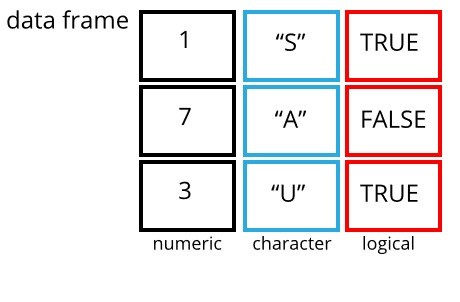
\includegraphics{./fig/data-frame.png}
\caption{data frame example}
\end{figure}

A data frame can be created by hand, but most commonly they are
generated by the functions \texttt{read\_csv()} or
\texttt{read\_table()}; in other words, when importing spreadsheets from
your hard drive (or the web).

A tibble is an extension of \texttt{R} data frames used by the
\emph{tidyverse}. When the data is read using \texttt{read\_csv()}, it
is stored in an object of class \texttt{tbl\_df}, \texttt{tbl}, and
\texttt{data.frame}. You can see the class of an object with

\begin{Shaded}
\begin{Highlighting}[]
\KeywordTok{class}\NormalTok{(interviews)}
\end{Highlighting}
\end{Shaded}

\begin{verbatim}
## [1] "spec_tbl_df" "tbl_df"      "tbl"         "data.frame"
\end{verbatim}

As a \texttt{tibble}, the type of data included in each column is listed
in an abbreviated fashion below the column names. For instance, here
\texttt{key\_ID} is a column of integers (abbreviated
\texttt{\textless{}int\textgreater{}}), \texttt{village} is a column of
characters (\texttt{\textless{}chr\textgreater{}}) and the
\texttt{interview\_date} is a column in the ``date and time'' format
(\texttt{\textless{}dttm\textgreater{}}).

\section{Inspecting data frames}\label{inspecting-data-frames}

When calling a \texttt{tbl\_df} object (like \texttt{interviews} here),
there is already a lot of information about our data frame being
displayed such as the number of rows, the number of columns, the names
of the columns, and as we just saw the class of data stored in each
column. However, there are functions to extract this information from
data frames. Here is a non-exhaustive list of some of these functions.
Let's try them out!

\begin{itemize}
\item
  Size:
\item
  \texttt{dim(interviews)} - returns a vector with the number of rows in
  the first element, and the number of columns as the second element
  (the \textbf{dim} ensions of the object)
\item
  \texttt{nrow(interviews)} - returns the number of rows
\item
  \texttt{ncol(interviews)} - returns the number of columns
\item
  Content:
\item
  \texttt{head(interviews)} - shows the first 6 rows
\item
  \texttt{tail(interviews)} - shows the last 6 rows
\item
  Names:
\item
  \texttt{names(interviews)} - returns the column names (synonym of
  \texttt{colnames()} for \texttt{data.frame} objects)
\item
  Summary:
\item
  \texttt{str(interviews)} - structure of the object and information
  about the class, length and content of each column
\item
  \texttt{summary(interviews)} - summary statistics for each column
\end{itemize}

Note: most of these functions are ``generic'', they can be used on other
types of objects besides data frames.

\section{Indexing and subsetting data
frames}\label{indexing-and-subsetting-data-frames}

Our interviews data frame has rows and columns (it has 2 dimensions), if
we want to extract some specific data from it, we need to specify the
``coordinates'' we want from it. Row numbers come first, followed by
column numbers. However, note that different ways of specifying these
coordinates lead to results with different classes.

\begin{Shaded}
\begin{Highlighting}[]
\NormalTok{## first element in the first column of the data frame (as a vector)}
\NormalTok{interviews[}\DecValTok{1}\NormalTok{, }\DecValTok{1}\NormalTok{]}
\end{Highlighting}
\end{Shaded}

\begin{verbatim}
## # A tibble: 1 x 1
##   key_ID
##    <dbl>
## 1      1
\end{verbatim}

\begin{Shaded}
\begin{Highlighting}[]
\NormalTok{## first element in the 6th column (as a vector)}
\NormalTok{interviews[}\DecValTok{1}\NormalTok{, }\DecValTok{6}\NormalTok{]}
\end{Highlighting}
\end{Shaded}

\begin{verbatim}
## # A tibble: 1 x 1
##   respondent_wall_type
##   <chr>               
## 1 muddaub
\end{verbatim}

\begin{Shaded}
\begin{Highlighting}[]
\NormalTok{## first column of the data frame (as a vector)}
\NormalTok{interviews[[}\DecValTok{1}\NormalTok{]]}
\end{Highlighting}
\end{Shaded}

\begin{verbatim}
##   [1]   1   1   3   4   5   6   7   8   9  10  11  12  13  14  15  16  17  18
##  [19]  19  20  21  22  23  24  25  26  27  28  29  30  31  32  33  34  35  36
##  [37]  37  38  39  40  41  42  43  44  45  46  47  48  49  50  51  52  21  54
##  [55]  55  56  57  58  59  60  61  62  63  64  65  66  67  68  69  70  71 127
##  [73] 133 152 153 155 178 177 180 181 182 186 187 195 196 197 198 201 202  72
##  [91]  73  76  83  85  89 101 103 102  78  80 104 105 106 109 110 113 118 125
## [109] 119 115 108 116 117 144 143 150 159 160 165 166 167 174 175 189 191 192
## [127] 126 193 194 199 200
\end{verbatim}

\begin{Shaded}
\begin{Highlighting}[]
\NormalTok{## first column of the data frame (as a data.frame)}
\NormalTok{interviews[}\DecValTok{1}\NormalTok{]}
\end{Highlighting}
\end{Shaded}

\begin{verbatim}
## # A tibble: 131 x 1
##    key_ID
##     <dbl>
##  1      1
##  2      1
##  3      3
##  4      4
##  5      5
##  6      6
##  7      7
##  8      8
##  9      9
## 10     10
## # … with 121 more rows
\end{verbatim}

\begin{Shaded}
\begin{Highlighting}[]
\NormalTok{## first three elements in the 7th column (as a vector)}
\NormalTok{interviews[}\DecValTok{1}\OperatorTok{:}\DecValTok{3}\NormalTok{, }\DecValTok{7}\NormalTok{]}
\end{Highlighting}
\end{Shaded}

\begin{verbatim}
## # A tibble: 3 x 1
##   rooms
##   <dbl>
## 1     1
## 2     1
## 3     1
\end{verbatim}

\begin{Shaded}
\begin{Highlighting}[]
\NormalTok{## the 3rd row of the data frame (as a data.frame)}
\NormalTok{interviews[}\DecValTok{3}\NormalTok{, ]}
\end{Highlighting}
\end{Shaded}

\begin{verbatim}
## # A tibble: 1 x 14
##   key_ID village interview_date      no_membrs years_liv respondent_wall… rooms
##    <dbl> <chr>   <dttm>                  <dbl>     <dbl> <chr>            <dbl>
## 1      3 God     2016-11-17 00:00:00        10        15 burntbricks          1
## # … with 7 more variables: memb_assoc <chr>, affect_conflicts <chr>,
## #   liv_count <dbl>, items_owned <chr>, no_meals <dbl>, months_lack_food <chr>,
## #   instanceID <chr>
\end{verbatim}

\begin{Shaded}
\begin{Highlighting}[]
\NormalTok{## equivalent to head_interviews <- head(interviews)}
\NormalTok{head_interviews <-}\StringTok{ }\NormalTok{interviews[}\DecValTok{1}\OperatorTok{:}\DecValTok{6}\NormalTok{, ]}
\end{Highlighting}
\end{Shaded}

\texttt{:} is a special function that creates numeric vectors of
integers in increasing or decreasing order, test \texttt{1:10} and
\texttt{10:1} for instance.

You can also exclude certain indices of a data frame using the
``\texttt{-}'' sign:

\begin{Shaded}
\begin{Highlighting}[]
\NormalTok{interviews[, }\OperatorTok{-}\DecValTok{1}\NormalTok{]          }\CommentTok{# The whole data frame, except the first column}
\end{Highlighting}
\end{Shaded}

\begin{verbatim}
## # A tibble: 131 x 13
##    village interview_date      no_membrs years_liv respondent_wall… rooms
##    <chr>   <dttm>                  <dbl>     <dbl> <chr>            <dbl>
##  1 God     2016-11-17 00:00:00         3         4 muddaub              1
##  2 God     2016-11-17 00:00:00         7         9 muddaub              1
##  3 God     2016-11-17 00:00:00        10        15 burntbricks          1
##  4 God     2016-11-17 00:00:00         7         6 burntbricks          1
##  5 God     2016-11-17 00:00:00         7        40 burntbricks          1
##  6 God     2016-11-17 00:00:00         3         3 muddaub              1
##  7 God     2016-11-17 00:00:00         6        38 muddaub              1
##  8 Chirod… 2016-11-16 00:00:00        12        70 burntbricks          3
##  9 Chirod… 2016-11-16 00:00:00         8         6 burntbricks          1
## 10 Chirod… 2016-12-16 00:00:00        12        23 burntbricks          5
## # … with 121 more rows, and 7 more variables: memb_assoc <chr>,
## #   affect_conflicts <chr>, liv_count <dbl>, items_owned <chr>, no_meals <dbl>,
## #   months_lack_food <chr>, instanceID <chr>
\end{verbatim}

\begin{Shaded}
\begin{Highlighting}[]
\NormalTok{interviews[}\OperatorTok{-}\KeywordTok{c}\NormalTok{(}\DecValTok{7}\OperatorTok{:}\DecValTok{131}\NormalTok{), ]   }\CommentTok{# Equivalent to head(interviews)}
\end{Highlighting}
\end{Shaded}

\begin{verbatim}
## # A tibble: 6 x 14
##   key_ID village interview_date      no_membrs years_liv respondent_wall… rooms
##    <dbl> <chr>   <dttm>                  <dbl>     <dbl> <chr>            <dbl>
## 1      1 God     2016-11-17 00:00:00         3         4 muddaub              1
## 2      1 God     2016-11-17 00:00:00         7         9 muddaub              1
## 3      3 God     2016-11-17 00:00:00        10        15 burntbricks          1
## 4      4 God     2016-11-17 00:00:00         7         6 burntbricks          1
## 5      5 God     2016-11-17 00:00:00         7        40 burntbricks          1
## 6      6 God     2016-11-17 00:00:00         3         3 muddaub              1
## # … with 7 more variables: memb_assoc <chr>, affect_conflicts <chr>,
## #   liv_count <dbl>, items_owned <chr>, no_meals <dbl>, months_lack_food <chr>,
## #   instanceID <chr>
\end{verbatim}

Data frames can be subset by calling indices (as shown previously), but
also by calling their column names directly:

\begin{Shaded}
\begin{Highlighting}[]
\NormalTok{interviews[}\StringTok{"village"}\NormalTok{]       }\CommentTok{# Result is a data frame}
\NormalTok{interviews[, }\StringTok{"village"}\NormalTok{]     }\CommentTok{# Result is a data frame}
\NormalTok{interviews[[}\StringTok{"village"}\NormalTok{]]     }\CommentTok{# Result is a vector}
\NormalTok{interviews}\OperatorTok{$}\NormalTok{village          }\CommentTok{# Result is a vector}
\end{Highlighting}
\end{Shaded}

In RStudio, you can use the autocompletion feature to get the full and
correct names of the columns.

\begin{quote}
\section{Exercise}\label{exercise-6}

\begin{enumerate}
\def\labelenumi{\arabic{enumi}.}
\item
  Create a data frame (\texttt{interviews\_100}) containing only the
  data in row 100 of the \texttt{interviews} dataset.
\item
  Notice how \texttt{nrow()} gave you the number of rows in a data
  frame?

  \begin{itemize}
  \tightlist
  \item
    Use that number to pull out just that last row in the data frame.
  \item
    Compare that with what you see as the last row using \texttt{tail()}
    to make sure it's meeting expectations.
  \item
    Pull out that last row using \texttt{nrow()} instead of the row
    number.
  \item
    Create a new data frame (\texttt{interviews\_last}) from that last
    row.
  \end{itemize}
\item
  Use \texttt{nrow()} to extract the row that is in the middle of the
  data frame. Store the content of this row in an object named
  \texttt{interviews\_middle}.
\item
  Combine \texttt{nrow()} with the \texttt{-} notation above to
  reproduce the behavior of \texttt{head(interviews)}, keeping just the
  first through 6th rows of the interviews dataset.
\end{enumerate}

\begin{quote}
\section{Solution}\label{solution-5}

\begin{Shaded}
\begin{Highlighting}[]
\NormalTok{## 1.}
\NormalTok{interviews_}\DecValTok{100}\NormalTok{ <-}\StringTok{ }\NormalTok{interviews[}\DecValTok{100}\NormalTok{, ]}
\NormalTok{## 2.}
\CommentTok{# Saving `n_rows` to improve readability and reduce duplication}
\NormalTok{n_rows <-}\StringTok{ }\KeywordTok{nrow}\NormalTok{(interviews)}
\NormalTok{interviews_last <-}\StringTok{ }\NormalTok{interviews[n_rows, ]}
\NormalTok{## 3.}
\NormalTok{interviews_middle <-}\StringTok{ }\NormalTok{interviews[(n_rows }\OperatorTok{/}\StringTok{ }\DecValTok{2}\NormalTok{), ]}
\NormalTok{## 4.}
\NormalTok{interviews_head <-}\StringTok{ }\NormalTok{interviews[}\OperatorTok{-}\NormalTok{(}\DecValTok{7}\OperatorTok{:}\NormalTok{n_rows), ]}
\end{Highlighting}
\end{Shaded}
\end{quote}
\end{quote}

\chapter{\texorpdfstring{Data Wrangling with
\texttt{dplyr}}{Data Wrangling with dplyr}}\label{dplyr}

teaching: 50\\
exercises: 30\\
adapted from:
\url{https://datacarpentry.org/r-socialsci/03-dplyr-tidyr/index.html}

questions:

\begin{itemize}
\tightlist
\item
  How can I select specific rows and/or columns from a data frame?\\
\item
  How can I combine multiple commands into a single command?\\
\item
  How can create new columns or remove existing columns from a data
  frame?\\
\item
  How can I reformat a dataframe to meet my needs?
\end{itemize}

objectives:

\begin{itemize}
\tightlist
\item
  Describe the purpose of an R package and the \textbf{\texttt{dplyr}}
  and \textbf{\texttt{tidyr}} packages.\\
\item
  Select certain columns in a data frame with the
  \textbf{\texttt{dplyr}} function \texttt{select}.\\
\item
  Select certain rows in a data frame according to filtering conditions
  with the \textbf{\texttt{dplyr}} function \texttt{filter}.\\
\item
  Link the output of one \textbf{\texttt{dplyr}} function to the input
  of another function with the `pipe' operator
  \texttt{\%\textgreater{}\%}.\\
\item
  Add new columns to a data frame that are functions of existing columns
  with \texttt{mutate}.\\
\item
  Use the split-apply-combine concept for data analysis.\\
\item
  Use \texttt{summarize}, \texttt{group\_by}, and \texttt{count} to
  split a data frame into groups of observations, apply a summary
  statistics for each group, and then combine the results.\\
\item
  Describe the concept of a wide and a long table format and for which
  purpose those formats are useful.
\item
  Describe what key-value pairs are.\\
\item
  Reshape a data frame from long to wide format and back with the
  \texttt{spread} and \texttt{gather} commands from the
  \textbf{\texttt{tidyr}} package.\\
\item
  Export a data frame to a csv file.
\end{itemize}

keypoints:

\begin{itemize}
\tightlist
\item
  Use the \texttt{dplyr} package to manipulate dataframes.\\
\item
  Use \texttt{select()} to choose variables from a dataframe.\\
\item
  Use \texttt{filter()} to choose data based on values.\\
\item
  Use \texttt{group\_by()} and \texttt{summarize()} to work with subsets
  of data.\\
\item
  Use \texttt{mutate()} to create new variables.\\
\item
  Use the \texttt{tidyr} package to change the layout of dataframes.\\
\item
  Use \texttt{gather()} to go from wide to long format.\\
\item
  Use \texttt{spread()} to go from long to wide format.
\end{itemize}

\section{\texorpdfstring{Data Manipulation using \textbf{\texttt{dplyr}}
and
\textbf{\texttt{tidyr}}}{Data Manipulation using dplyr and tidyr}}\label{data-manipulation-using-dplyr-and-tidyr}

\textbf{\texttt{dplyr}} is a package for making tabular data
manipulation easier by using a limited set of functions that can be
combined to extract and summarize insights from your data. It pairs
nicely with \textbf{\texttt{tidyr}} which enables you to swiftly convert
between different data formats (long vs.~wide) for plotting and
analysis.

Similarly to \textbf{\texttt{readr}}, \textbf{\texttt{dplyr}} and
\textbf{\texttt{tidyr}} are also part of the tidyverse. These packages
were loaded in R's memory when we called \texttt{library(tidyverse)}
earlier.

\section{What is an R package?}\label{what-is-an-r-package}

An R package is a complete unit for sharing code with others. Each R
package contains the code for a set of R functions, the documentation
(or description) for each of the functions, as well as a practice
dataset to learn the functions on.

Generally, each R package is built with a specific task in mind. For
instance, the package \textbf{\texttt{dplyr}} provides easy tools for
the most common data manipulation tasks. It is built to work directly
with data frames, with many common tasks optimized by being written in a
compiled language (C++) (not all R packages are written in R!).

The package \textbf{\texttt{tidyr}} addresses the common problem of
wanting to reshape your data for plotting and use by different R
functions. Sometimes we want data sets where we have one row per
measurement. Sometimes we want a data frame where each measurement type
has its own column, and rows are instead more aggregated groups. Moving
back and forth between these formats is nontrivial, and
\textbf{\texttt{tidyr}} gives you tools for this and more sophisticated
data manipulation.

But there are also packages available for a wide range of tasks
including building plots (\textbf{\texttt{ggplot2}}, which we'll see
later), downloading data from the NCBI database, or performing
statistical analysis on your data set. Many packages such as these are
housed on, and downloadable from, the \textbf{C}omprehensive \textbf{R}
\textbf{A}rchive \textbf{N}etwork (CRAN) using
\texttt{install.packages}. This function makes the package accessible by
your R installation with the command \texttt{library()}, as you did with
\texttt{tidyverse} earlier.

To easily access the documentation for a package within R or RStudio,
use \texttt{help(package\ =\ "package\_name")}.

To learn more about \textbf{\texttt{dplyr}} and \textbf{\texttt{tidyr}}
after the workshop, you may want to check out this
\href{https://github.com/rstudio/cheatsheets/raw/master/data-transformation.pdf}{handy
data transformation with \textbf{\texttt{dplyr}} cheatsheet} and this
\href{https://github.com/rstudio/cheatsheets/raw/master/data-import.pdf}{one
about \textbf{\texttt{tidyr}}}.

\section{\texorpdfstring{Learning \textbf{\texttt{dplyr}} and
\textbf{\texttt{tidyr}}}{Learning dplyr and tidyr}}\label{learning-dplyr-and-tidyr}

To make sure, everyone will use the same dataset for this lesson, we'll
read again the SAFI dataset that we downloaded earlier.

\begin{Shaded}
\begin{Highlighting}[]
\NormalTok{## load the tidyverse}
\KeywordTok{library}\NormalTok{(tidyverse)}

\NormalTok{interviews <-}\StringTok{ }\KeywordTok{read_csv}\NormalTok{(}\StringTok{"data/SAFI_clean.csv"}\NormalTok{, }\DataTypeTok{na =} \StringTok{"NULL"}\NormalTok{)}

\NormalTok{## inspect the data}
\NormalTok{interviews}

\NormalTok{## preview the data}
\CommentTok{# View(interviews)}
\end{Highlighting}
\end{Shaded}

We're going to learn some of the most common \textbf{\texttt{dplyr}}
functions:

\begin{itemize}
\tightlist
\item
  \texttt{select()}: subset columns
\item
  \texttt{filter()}: subset rows on conditions
\item
  \texttt{mutate()}: create new columns by using information from other
  columns
\item
  \texttt{group\_by()} and \texttt{summarize()}: create summary
  statistics on grouped data
\item
  \texttt{arrange()}: sort results
\item
  \texttt{count()}: count discrete values
\end{itemize}

\section{Selecting columns and filtering
rows}\label{selecting-columns-and-filtering-rows}

To select columns of a data frame, use \texttt{select()}. The first
argument to this function is the data frame (\texttt{interviews}), and
the subsequent arguments are the columns to keep.

\begin{Shaded}
\begin{Highlighting}[]
\KeywordTok{select}\NormalTok{(interviews, village, no_membrs, years_liv)}
\end{Highlighting}
\end{Shaded}

To choose rows based on a specific criteria, use \texttt{filter()}:

\begin{Shaded}
\begin{Highlighting}[]
\KeywordTok{filter}\NormalTok{(interviews, village }\OperatorTok{==}\StringTok{ "God"}\NormalTok{)}
\end{Highlighting}
\end{Shaded}

\begin{verbatim}
## # A tibble: 43 x 14
##    key_ID village interview_date      no_membrs years_liv respondent_wall… rooms
##     <dbl> <chr>   <dttm>                  <dbl>     <dbl> <chr>            <dbl>
##  1      1 God     2016-11-17 00:00:00         3         4 muddaub              1
##  2      1 God     2016-11-17 00:00:00         7         9 muddaub              1
##  3      3 God     2016-11-17 00:00:00        10        15 burntbricks          1
##  4      4 God     2016-11-17 00:00:00         7         6 burntbricks          1
##  5      5 God     2016-11-17 00:00:00         7        40 burntbricks          1
##  6      6 God     2016-11-17 00:00:00         3         3 muddaub              1
##  7      7 God     2016-11-17 00:00:00         6        38 muddaub              1
##  8     11 God     2016-11-21 00:00:00         6        20 sunbricks            1
##  9     12 God     2016-11-21 00:00:00         7        20 burntbricks          3
## 10     13 God     2016-11-21 00:00:00         6         8 burntbricks          1
## # … with 33 more rows, and 7 more variables: memb_assoc <chr>,
## #   affect_conflicts <chr>, liv_count <dbl>, items_owned <chr>, no_meals <dbl>,
## #   months_lack_food <chr>, instanceID <chr>
\end{verbatim}

\section{Pipes}\label{pipes}

What if you want to select and filter at the same time? There are three
ways to do this: use intermediate steps, nested functions, or pipes.

With intermediate steps, you create a temporary data frame and use that
as input to the next function, like this:

\begin{Shaded}
\begin{Highlighting}[]
\NormalTok{interviews2 <-}\StringTok{ }\KeywordTok{filter}\NormalTok{(interviews, village }\OperatorTok{==}\StringTok{ "God"}\NormalTok{)}
\NormalTok{interviews_god <-}\StringTok{ }\KeywordTok{select}\NormalTok{(interviews2, no_membrs, years_liv)}
\end{Highlighting}
\end{Shaded}

This is readable, but can clutter up your workspace with lots of objects
that you have to name individually. With multiple steps, that can be
hard to keep track of.

You can also nest functions (i.e.~one function inside of another), like
this:

\begin{Shaded}
\begin{Highlighting}[]
\NormalTok{interviews_god <-}\StringTok{ }\KeywordTok{select}\NormalTok{(}\KeywordTok{filter}\NormalTok{(interviews, village }\OperatorTok{==}\StringTok{ "God"}\NormalTok{), no_membrs, years_liv)}
\end{Highlighting}
\end{Shaded}

This is handy, but can be difficult to read if too many functions are
nested, as R evaluates the expression from the inside out (in this case,
filtering, then selecting).

The last option, \emph{pipes}, are a recent addition to R. Pipes let you
take the output of one function and send it directly to the next, which
is useful when you need to do many things to the same dataset. Pipes in
R look like \texttt{\%\textgreater{}\%} and are made available via the
\textbf{\texttt{magrittr}} package, installed automatically with
\textbf{\texttt{dplyr}}. If you use RStudio, you can type the pipe with
Ctrl + Shift + M if you have a PC or Cmd + Shift + M if you have a Mac.

\begin{Shaded}
\begin{Highlighting}[]
\NormalTok{interviews }\OperatorTok
\StringTok{    }\KeywordTok{filter}\NormalTok{(village }\OperatorTok{==}\StringTok{ "God"}\NormalTok{) }\OperatorTok
\StringTok{    }\KeywordTok{select}\NormalTok{(no_membrs, years_liv)}
\end{Highlighting}
\end{Shaded}

\begin{verbatim}
## # A tibble: 43 x 2
##    no_membrs years_liv
##        <dbl>     <dbl>
##  1         3         4
##  2         7         9
##  3        10        15
##  4         7         6
##  5         7        40
##  6         3         3
##  7         6        38
##  8         6        20
##  9         7        20
## 10         6         8
## # … with 33 more rows
\end{verbatim}

In the above code, we use the pipe to send the \texttt{interviews}
dataset first through \texttt{filter()} to keep rows where
\texttt{village} is ``God'', then through \texttt{select()} to keep only
the \texttt{no\_membrs} and \texttt{years\_liv} columns. Since
\texttt{\%\textgreater{}\%} takes the object on its left and passes it
as the first argument to the function on its right, we don't need to
explicitly include the data frame as an argument to the
\texttt{filter()} and \texttt{select()} functions any more.

Some may find it helpful to read the pipe like the word ``then''. For
instance, in the above example, we take the data frame
\texttt{interviews}, \emph{then} we \texttt{filter} for rows with
\texttt{village\ ==\ "God"}, \emph{then} we \texttt{select} columns
\texttt{no\_membrs} and \texttt{years\_liv}. The \textbf{\texttt{dplyr}}
functions by themselves are somewhat simple, but by combining them into
linear workflows with the pipe, we can accomplish more complex
manipulations of data frames.

If we want to create a new object with this smaller version of the data,
we can assign it a new name:

\begin{Shaded}
\begin{Highlighting}[]
\NormalTok{interviews_god <-}\StringTok{ }\NormalTok{interviews }\OperatorTok
\StringTok{    }\KeywordTok{filter}\NormalTok{(village }\OperatorTok{==}\StringTok{ "God"}\NormalTok{) }\OperatorTok
\StringTok{    }\KeywordTok{select}\NormalTok{(no_membrs, years_liv)}

\NormalTok{interviews_god}
\end{Highlighting}
\end{Shaded}

\begin{verbatim}
## # A tibble: 43 x 2
##    no_membrs years_liv
##        <dbl>     <dbl>
##  1         3         4
##  2         7         9
##  3        10        15
##  4         7         6
##  5         7        40
##  6         3         3
##  7         6        38
##  8         6        20
##  9         7        20
## 10         6         8
## # … with 33 more rows
\end{verbatim}

Note that the final data frame (\texttt{interviews\_god}) is the
leftmost part of this expression.

\begin{quote}
\section{Exercise}\label{exercise-7}

Using pipes, subset the \texttt{interviews} data to include interviews
where respondents were members of an irrigation association
(\texttt{memb\_assoc}) and retain only the columns
\texttt{affect\_conflicts}, \texttt{liv\_count}, and \texttt{no\_meals}.

\begin{quote}
\section{Solution}\label{solution-6}

\begin{Shaded}
\begin{Highlighting}[]
\NormalTok{interviews }\OperatorTok
\StringTok{    }\KeywordTok{filter}\NormalTok{(memb_assoc }\OperatorTok{==}\StringTok{ "yes"}\NormalTok{) }\OperatorTok
\StringTok{    }\KeywordTok{select}\NormalTok{(affect_conflicts, liv_count, no_meals)}
\end{Highlighting}
\end{Shaded}

\begin{verbatim}
## # A tibble: 33 x 3
##    affect_conflicts liv_count no_meals
##    <chr>                <dbl>    <dbl>
##  1 once                     3        2
##  2 never                    2        2
##  3 never                    2        3
##  4 once                     3        2
##  5 frequently               1        3
##  6 more_once                5        2
##  7 more_once                3        2
##  8 more_once                2        3
##  9 once                     3        3
## 10 never                    3        3
## # … with 23 more rows
\end{verbatim}
\end{quote}
\end{quote}

\subsection{Mutate}\label{mutate}

Frequently you'll want to create new columns based on the values in
existing columns, for example to do unit conversions, or to find the
ratio of values in two columns. For this we'll use \texttt{mutate()}.

We might be interested in the ratio of number of household members to
rooms used for sleeping (i.e.~avg number of people per room):

\begin{Shaded}
\begin{Highlighting}[]
\NormalTok{interviews }\OperatorTok
\StringTok{    }\KeywordTok{mutate}\NormalTok{(}\DataTypeTok{people_per_room =}\NormalTok{ no_membrs }\OperatorTok{/}\StringTok{ }\NormalTok{rooms)}
\end{Highlighting}
\end{Shaded}

\begin{verbatim}
## # A tibble: 131 x 15
##    key_ID village interview_date      no_membrs years_liv respondent_wall… rooms
##     <dbl> <chr>   <dttm>                  <dbl>     <dbl> <chr>            <dbl>
##  1      1 God     2016-11-17 00:00:00         3         4 muddaub              1
##  2      1 God     2016-11-17 00:00:00         7         9 muddaub              1
##  3      3 God     2016-11-17 00:00:00        10        15 burntbricks          1
##  4      4 God     2016-11-17 00:00:00         7         6 burntbricks          1
##  5      5 God     2016-11-17 00:00:00         7        40 burntbricks          1
##  6      6 God     2016-11-17 00:00:00         3         3 muddaub              1
##  7      7 God     2016-11-17 00:00:00         6        38 muddaub              1
##  8      8 Chirod… 2016-11-16 00:00:00        12        70 burntbricks          3
##  9      9 Chirod… 2016-11-16 00:00:00         8         6 burntbricks          1
## 10     10 Chirod… 2016-12-16 00:00:00        12        23 burntbricks          5
## # … with 121 more rows, and 8 more variables: memb_assoc <chr>,
## #   affect_conflicts <chr>, liv_count <dbl>, items_owned <chr>, no_meals <dbl>,
## #   months_lack_food <chr>, instanceID <chr>, people_per_room <dbl>
\end{verbatim}

We may be interested in investigating whether being a member of an
irrigation association had any effect on the ratio of household members
to rooms. To look at this relationship, we will first remove data from
our dataset where the respondent didn't answer the question of whether
they were a member of an irrigation association. These cases are
recorded as ``NULL'' in the dataset.

To remove these cases, we could insert a \texttt{filter()} in the chain:

\begin{Shaded}
\begin{Highlighting}[]
\NormalTok{interviews }\OperatorTok
\StringTok{    }\KeywordTok{filter}\NormalTok{(}\OperatorTok{!}\KeywordTok{is.na}\NormalTok{(memb_assoc)) }\OperatorTok
\StringTok{    }\KeywordTok{mutate}\NormalTok{(}\DataTypeTok{people_per_room =}\NormalTok{ no_membrs }\OperatorTok{/}\StringTok{ }\NormalTok{rooms)}
\end{Highlighting}
\end{Shaded}

\begin{verbatim}
## # A tibble: 92 x 15
##    key_ID village interview_date      no_membrs years_liv respondent_wall… rooms
##     <dbl> <chr>   <dttm>                  <dbl>     <dbl> <chr>            <dbl>
##  1      1 God     2016-11-17 00:00:00         7         9 muddaub              1
##  2      7 God     2016-11-17 00:00:00         6        38 muddaub              1
##  3      8 Chirod… 2016-11-16 00:00:00        12        70 burntbricks          3
##  4      9 Chirod… 2016-11-16 00:00:00         8         6 burntbricks          1
##  5     10 Chirod… 2016-12-16 00:00:00        12        23 burntbricks          5
##  6     12 God     2016-11-21 00:00:00         7        20 burntbricks          3
##  7     13 God     2016-11-21 00:00:00         6         8 burntbricks          1
##  8     15 God     2016-11-21 00:00:00         5        30 sunbricks            2
##  9     21 God     2016-11-21 00:00:00         8        20 burntbricks          1
## 10     24 Ruaca   2016-11-21 00:00:00         6         4 burntbricks          2
## # … with 82 more rows, and 8 more variables: memb_assoc <chr>,
## #   affect_conflicts <chr>, liv_count <dbl>, items_owned <chr>, no_meals <dbl>,
## #   months_lack_food <chr>, instanceID <chr>, people_per_room <dbl>
\end{verbatim}

The \texttt{!} symbol negates the result, so we're asking for every row
where \texttt{memb\_assoc} \emph{is not} missing..

\begin{quote}
\section{Exercise}\label{exercise-8}

Create a new data frame from the \texttt{interviews} data that meets the
following criteria: contains only the \texttt{village} column and a new
column called \texttt{total\_meals} containing a value that is equal to
the total number of meals served in the household per day on average
(\texttt{no\_membrs} times \texttt{no\_meals}). Only the rows where
\texttt{total\_meals} is greater than 20 should be shown in the final
data frame.

\textbf{Hint}: think about how the commands should be ordered to produce
this data frame!

\begin{quote}
\section{Solution}\label{solution-7}

\begin{Shaded}
\begin{Highlighting}[]
\NormalTok{interviews_total_meals <-}\StringTok{ }\NormalTok{interviews }\OperatorTok
\StringTok{    }\KeywordTok{mutate}\NormalTok{(}\DataTypeTok{total_meals =}\NormalTok{ no_membrs }\OperatorTok{*}\StringTok{ }\NormalTok{no_meals) }\OperatorTok
\StringTok{    }\KeywordTok{filter}\NormalTok{(total_meals }\OperatorTok{>}\StringTok{ }\DecValTok{20}\NormalTok{) }\OperatorTok
\StringTok{    }\KeywordTok{select}\NormalTok{(village, total_meals)}
\end{Highlighting}
\end{Shaded}
\end{quote}
\end{quote}

\subsection{Split-apply-combine data analysis and the summarize()
function}\label{split-apply-combine-data-analysis-and-the-summarize-function}

Many data analysis tasks can be approached using the
\emph{split-apply-combine} paradigm: split the data into groups, apply
some analysis to each group, and then combine the results.
\textbf{\texttt{dplyr}} makes this very easy through the use of the
\texttt{group\_by()} function.

\subsubsection{\texorpdfstring{The \texttt{summarize()}
function}{The summarize() function}}\label{the-summarize-function}

\texttt{group\_by()} is often used together with \texttt{summarize()},
which collapses each group into a single-row summary of that group.
\texttt{group\_by()} takes as arguments the column names that contain
the \textbf{categorical} variables for which you want to calculate the
summary statistics. So to compute the average household size by village:

\begin{Shaded}
\begin{Highlighting}[]
\NormalTok{interviews }\OperatorTok
\StringTok{    }\KeywordTok{group_by}\NormalTok{(village) }\OperatorTok
\StringTok{    }\KeywordTok{summarize}\NormalTok{(}\DataTypeTok{mean_no_membrs =} \KeywordTok{mean}\NormalTok{(no_membrs))}
\end{Highlighting}
\end{Shaded}

\begin{verbatim}
## # A tibble: 3 x 2
##   village  mean_no_membrs
##   <chr>             <dbl>
## 1 Chirodzo           7.08
## 2 God                6.86
## 3 Ruaca              7.57
\end{verbatim}

You may also have noticed that the output from these calls doesn't run
off the screen anymore. It's one of the advantages of \texttt{tbl\_df}
over data frame.

You can also group by multiple columns:

\begin{Shaded}
\begin{Highlighting}[]
\NormalTok{interviews }\OperatorTok
\StringTok{    }\KeywordTok{group_by}\NormalTok{(village, memb_assoc) }\OperatorTok
\StringTok{    }\KeywordTok{summarize}\NormalTok{(}\DataTypeTok{mean_no_membrs =} \KeywordTok{mean}\NormalTok{(no_membrs))}
\end{Highlighting}
\end{Shaded}

\begin{verbatim}
## # A tibble: 9 x 3
## # Groups:   village [3]
##   village  memb_assoc mean_no_membrs
##   <chr>    <chr>               <dbl>
## 1 Chirodzo no                   8.06
## 2 Chirodzo yes                  7.82
## 3 Chirodzo <NA>                 5.08
## 4 God      no                   7.13
## 5 God      yes                  8   
## 6 God      <NA>                 6   
## 7 Ruaca    no                   7.18
## 8 Ruaca    yes                  9.5 
## 9 Ruaca    <NA>                 6.22
\end{verbatim}

When grouping both by \texttt{village} and \texttt{membr\_assoc}, we see
rows in our table for respondents who did not specify whether they were
a member of an irrigation association. We can exclude those data from
our table using a filter step.

\begin{Shaded}
\begin{Highlighting}[]
\NormalTok{interviews }\OperatorTok
\StringTok{    }\KeywordTok{filter}\NormalTok{(}\OperatorTok{!}\KeywordTok{is.na}\NormalTok{(memb_assoc)) }\OperatorTok
\StringTok{    }\KeywordTok{group_by}\NormalTok{(village, memb_assoc) }\OperatorTok
\StringTok{    }\KeywordTok{summarize}\NormalTok{(}\DataTypeTok{mean_no_membrs =} \KeywordTok{mean}\NormalTok{(no_membrs))}
\end{Highlighting}
\end{Shaded}

\begin{verbatim}
## # A tibble: 6 x 3
## # Groups:   village [3]
##   village  memb_assoc mean_no_membrs
##   <chr>    <chr>               <dbl>
## 1 Chirodzo no                   8.06
## 2 Chirodzo yes                  7.82
## 3 God      no                   7.13
## 4 God      yes                  8   
## 5 Ruaca    no                   7.18
## 6 Ruaca    yes                  9.5
\end{verbatim}

Once the data are grouped, you can also summarize multiple variables at
the same time (and not necessarily on the same variable). For instance,
we could add a column indicating the minimum household size for each
village for each group (members of an irrigation association vs not):

\begin{Shaded}
\begin{Highlighting}[]
\NormalTok{interviews }\OperatorTok
\StringTok{    }\KeywordTok{filter}\NormalTok{(}\OperatorTok{!}\KeywordTok{is.na}\NormalTok{(memb_assoc)) }\OperatorTok
\StringTok{    }\KeywordTok{group_by}\NormalTok{(village, memb_assoc) }\OperatorTok
\StringTok{    }\KeywordTok{summarize}\NormalTok{(}\DataTypeTok{mean_no_membrs =} \KeywordTok{mean}\NormalTok{(no_membrs),}
              \DataTypeTok{min_membrs =} \KeywordTok{min}\NormalTok{(no_membrs))}
\end{Highlighting}
\end{Shaded}

\begin{verbatim}
## # A tibble: 6 x 4
## # Groups:   village [3]
##   village  memb_assoc mean_no_membrs min_membrs
##   <chr>    <chr>               <dbl>      <dbl>
## 1 Chirodzo no                   8.06          4
## 2 Chirodzo yes                  7.82          2
## 3 God      no                   7.13          3
## 4 God      yes                  8             5
## 5 Ruaca    no                   7.18          2
## 6 Ruaca    yes                  9.5           5
\end{verbatim}

It is sometimes useful to rearrange the result of a query to inspect the
values. For instance, we can sort on \texttt{min\_membrs} to put the
group with the smallest household first:

\begin{Shaded}
\begin{Highlighting}[]
\NormalTok{interviews }\OperatorTok
\StringTok{    }\KeywordTok{filter}\NormalTok{(}\OperatorTok{!}\KeywordTok{is.na}\NormalTok{(memb_assoc)) }\OperatorTok
\StringTok{    }\KeywordTok{group_by}\NormalTok{(village, memb_assoc) }\OperatorTok
\StringTok{    }\KeywordTok{summarize}\NormalTok{(}\DataTypeTok{mean_no_membrs =} \KeywordTok{mean}\NormalTok{(no_membrs), }\DataTypeTok{min_membrs =} \KeywordTok{min}\NormalTok{(no_membrs)) }\OperatorTok
\StringTok{    }\KeywordTok{arrange}\NormalTok{(min_membrs)}
\end{Highlighting}
\end{Shaded}

\begin{verbatim}
## # A tibble: 6 x 4
## # Groups:   village [3]
##   village  memb_assoc mean_no_membrs min_membrs
##   <chr>    <chr>               <dbl>      <dbl>
## 1 Chirodzo yes                  7.82          2
## 2 Ruaca    no                   7.18          2
## 3 God      no                   7.13          3
## 4 Chirodzo no                   8.06          4
## 5 God      yes                  8             5
## 6 Ruaca    yes                  9.5           5
\end{verbatim}

To sort in descending order, we need to add the \texttt{desc()}
function. If we want to sort the results by decreasing order of minimum
household size:

\begin{Shaded}
\begin{Highlighting}[]
\NormalTok{interviews }\OperatorTok
\StringTok{    }\KeywordTok{filter}\NormalTok{(}\OperatorTok{!}\KeywordTok{is.na}\NormalTok{(memb_assoc)) }\OperatorTok
\StringTok{    }\KeywordTok{group_by}\NormalTok{(village, memb_assoc) }\OperatorTok
\StringTok{    }\KeywordTok{summarize}\NormalTok{(}\DataTypeTok{mean_no_membrs =} \KeywordTok{mean}\NormalTok{(no_membrs),}
              \DataTypeTok{min_membrs =} \KeywordTok{min}\NormalTok{(no_membrs)) }\OperatorTok
\StringTok{    }\KeywordTok{arrange}\NormalTok{(}\KeywordTok{desc}\NormalTok{(min_membrs))}
\end{Highlighting}
\end{Shaded}

\begin{verbatim}
## # A tibble: 6 x 4
## # Groups:   village [3]
##   village  memb_assoc mean_no_membrs min_membrs
##   <chr>    <chr>               <dbl>      <dbl>
## 1 God      yes                  8             5
## 2 Ruaca    yes                  9.5           5
## 3 Chirodzo no                   8.06          4
## 4 God      no                   7.13          3
## 5 Chirodzo yes                  7.82          2
## 6 Ruaca    no                   7.18          2
\end{verbatim}

\subsubsection{Counting}\label{counting}

When working with data, we often want to know the number of observations
found for each factor or combination of factors. For this task,
\textbf{\texttt{dplyr}} provides \texttt{count()}. For example, if we
wanted to count the number of rows of data for each village, we would
do:

\begin{Shaded}
\begin{Highlighting}[]
\NormalTok{interviews }\OperatorTok
\StringTok{    }\KeywordTok{count}\NormalTok{(village)}
\end{Highlighting}
\end{Shaded}

\begin{verbatim}
## # A tibble: 3 x 2
##   village      n
##   <chr>    <int>
## 1 Chirodzo    39
## 2 God         43
## 3 Ruaca       49
\end{verbatim}

For convenience, \texttt{count()} provides the \texttt{sort} argument to
get results in decreasing order:

\begin{Shaded}
\begin{Highlighting}[]
\NormalTok{interviews }\OperatorTok
\StringTok{    }\KeywordTok{count}\NormalTok{(village, }\DataTypeTok{sort =} \OtherTok{TRUE}\NormalTok{)}
\end{Highlighting}
\end{Shaded}

\begin{verbatim}
## # A tibble: 3 x 2
##   village      n
##   <chr>    <int>
## 1 Ruaca       49
## 2 God         43
## 3 Chirodzo    39
\end{verbatim}

\begin{quote}
\section{Exercise}\label{exercise-9}

\begin{enumerate}
\def\labelenumi{\arabic{enumi}.}
\tightlist
\item
  How many households in the survey have an average of two meals per
  day? Three meals per day? Are there any other numbers of meals
  represented?
\end{enumerate}

\begin{quote}
\section{Solution}\label{solution-8}

\begin{Shaded}
\begin{Highlighting}[]
\NormalTok{interviews }\OperatorTok
\StringTok{   }\KeywordTok{count}\NormalTok{(no_meals)}
\end{Highlighting}
\end{Shaded}

\begin{verbatim}
## # A tibble: 2 x 2
##   no_meals     n
##      <dbl> <int>
## 1        2    52
## 2        3    79
\end{verbatim}
\end{quote}
\end{quote}

\begin{quote}
\begin{enumerate}
\def\labelenumi{\arabic{enumi}.}
\setcounter{enumi}{1}
\tightlist
\item
  Use \texttt{group\_by()} and \texttt{summarize()} to find the mean,
  min, and max number of household members for each village. Also add
  the number of observations (hint: see \texttt{?n}).
\end{enumerate}

\begin{quote}
\section{Solution}\label{solution-9}

\begin{Shaded}
\begin{Highlighting}[]
\NormalTok{interviews }\OperatorTok
\StringTok{  }\KeywordTok{group_by}\NormalTok{(village) }\OperatorTok
\StringTok{  }\KeywordTok{summarize}\NormalTok{(}
      \DataTypeTok{mean_no_membrs =} \KeywordTok{mean}\NormalTok{(no_membrs),}
      \DataTypeTok{min_no_membrs =} \KeywordTok{min}\NormalTok{(no_membrs),}
      \DataTypeTok{max_no_membrs =} \KeywordTok{max}\NormalTok{(no_membrs),}
      \DataTypeTok{n =} \KeywordTok{n}\NormalTok{()}
\NormalTok{  )}
\end{Highlighting}
\end{Shaded}

\begin{verbatim}
## # A tibble: 3 x 5
##   village  mean_no_membrs min_no_membrs max_no_membrs     n
##   <chr>             <dbl>         <dbl>         <dbl> <int>
## 1 Chirodzo           7.08             2            12    39
## 2 God                6.86             3            15    43
## 3 Ruaca              7.57             2            19    49
\end{verbatim}
\end{quote}

\begin{enumerate}
\def\labelenumi{\arabic{enumi}.}
\setcounter{enumi}{2}
\tightlist
\item
  What was the largest household interviewed in each month?
\end{enumerate}

\begin{quote}
\section{Solution}\label{solution-10}

\begin{Shaded}
\begin{Highlighting}[]
\CommentTok{# if not already included, add month, year, and day columns}
\KeywordTok{library}\NormalTok{(lubridate) }\CommentTok{# load lubridate if not already loaded}
\NormalTok{interviews }\OperatorTok
\StringTok{    }\KeywordTok{mutate}\NormalTok{(}\DataTypeTok{month =} \KeywordTok{month}\NormalTok{(interview_date),}
           \DataTypeTok{day =} \KeywordTok{day}\NormalTok{(interview_date),}
           \DataTypeTok{year =} \KeywordTok{year}\NormalTok{(interview_date)) }\OperatorTok
\StringTok{    }\KeywordTok{group_by}\NormalTok{(year, month) }\OperatorTok
\StringTok{    }\KeywordTok{summarize}\NormalTok{(}\DataTypeTok{max_no_membrs =} \KeywordTok{max}\NormalTok{(no_membrs))}
\end{Highlighting}
\end{Shaded}

\begin{verbatim}
## # A tibble: 5 x 3
## # Groups:   year [2]
##    year month max_no_membrs
##   <dbl> <dbl>         <dbl>
## 1  2016    11            19
## 2  2016    12            12
## 3  2017     4            17
## 4  2017     5            15
## 5  2017     6            15
\end{verbatim}
\end{quote}
\end{quote}

\section{Reshaping with gather and
spread}\label{reshaping-with-gather-and-spread}

In the
\href{http://www.datacarpentry.org/spreadsheets-socialsci/}{spreadsheet
lesson}, we discussed how to structure our data leading to the four
rules defining a tidy dataset:

\begin{enumerate}
\def\labelenumi{\arabic{enumi}.}
\tightlist
\item
  Each variable has its own column
\item
  Each observation has its own row
\item
  Each value must have its own cell
\item
  Each type of observational unit forms a table
\end{enumerate}

Here we examine the fourth rule: Each type of observational unit forms a
table.

In \texttt{interviews}, each row contains the values of variables
associated with each record (the unit), values such as the number of
household members or posessions associated with each record. What if
instead of comparing records, we wanted to look at differences in
households grouped by different types of housing construction materials?

We'd need to create a new table where each row (the unit) is comprised
of values of variables associated with each housing material (e.g.~for
\texttt{respondent\_wall\_type}). In practical terms this means the
values of the wall construction materials in
\texttt{respondent\_wall\_type} would become the names of column
variables and the cells would contain \texttt{TRUE} or \texttt{FALSE}.

Having created a new table, we can now explore the relationship within
and between household types - for example we could compare the ratio of
household members to sleeping rooms grouped by type of construction
material. The key point here is that we are still following a tidy data
structure, but we have \textbf{reshaped} the data according to the
observations of interest.

The opposite transformation would be to transform column names into
values of a variable.

We can do both these of transformations with two \texttt{tidyr}
functions, \texttt{spread()} and \texttt{gather()}.

\subsubsection{Spreading}\label{spreading}

\texttt{spread()} takes three principal arguments:

\begin{enumerate}
\def\labelenumi{\arabic{enumi}.}
\tightlist
\item
  the data
\item
  the \emph{key} column variable whose values will become new column
  names.
\item
  the \emph{value} column variable whose values will fill the new column
  variables.
\end{enumerate}

Further arguments include \texttt{fill} which, if set, fills in missing
values with the value provided.

Let's use \texttt{spread()} to transform interviews to create new
columns for each type of wall construction material. We use the pipe as
before too. Because both the \texttt{key} and \texttt{value} parameters
must come from column values, we will create a dummy column (we'll name
it \texttt{wall\_type\_logical}) to hold the value \texttt{TRUE}, which
we will then place into the appropriate column that corresponds to the
wall construction material for that respondent. When using
\texttt{mutate()} if you give a single value, it will be used for all
observations in the dataset. We will use \texttt{fill\ =\ FALSE} in
\texttt{spread()} to fill the rest of the new columns for that row with
\texttt{FALSE}.

\begin{Shaded}
\begin{Highlighting}[]
\NormalTok{interviews_spread <-}\StringTok{ }\NormalTok{interviews }\OperatorTok
\StringTok{    }\KeywordTok{mutate}\NormalTok{(}\DataTypeTok{wall_type_logical =} \OtherTok{TRUE}\NormalTok{) }\OperatorTok
\StringTok{    }\KeywordTok{spread}\NormalTok{(}\DataTypeTok{key =}\NormalTok{ respondent_wall_type, }\DataTypeTok{value =}\NormalTok{ wall_type_logical, }\DataTypeTok{fill =} \OtherTok{FALSE}\NormalTok{)}
\end{Highlighting}
\end{Shaded}

\begin{figure}
\centering
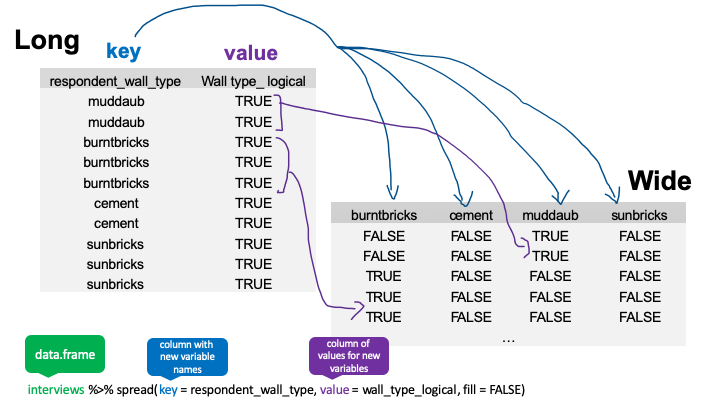
\includegraphics{./fig/long_to_wide.png}
\caption{}
\end{figure}

View the \texttt{interviews\_spread} data frame and notice that there is
no longer a column titled \texttt{respondent\_wall\_type}. This is
because there is a default parameter in \texttt{spread()} that drops the
original column.

\section{Gathering}\label{gathering}

The opposing situation could occur if we had been provided with data in
the form of \texttt{interviews\_spread}, where the building materials
are column names, but we wish to treat them as values of a
\texttt{respondent\_wall\_type} variable instead.

In this situation we are gathering the column names and turning them
into a pair of new variables. One variable represents the column names
as values, and the other variable contains the values previously
associated with the column names. We will do this in two steps to make
this process a bit clearer.

\texttt{gather()} takes four principal arguments:

\begin{enumerate}
\def\labelenumi{\arabic{enumi}.}
\tightlist
\item
  the data
\item
  the \emph{key} column variable we wish to create from column names.
\item
  the \emph{value} column variable we wish to create and fill with
  values associated with the key.
\item
  the names of the columns we use to fill the key variable (or to drop).
\end{enumerate}

To recreate our original data frame, we will use the following:

\begin{enumerate}
\def\labelenumi{\arabic{enumi}.}
\tightlist
\item
  the data - \texttt{interviews\_spread}
\item
  the \emph{key} column will be ``respondent\_wall\_type'' (as a
  character string). This is the name of the new column we want to
  create.
\item
  the \emph{value} column will be \texttt{wall\_type\_logical}. This
  will be either \texttt{TRUE} or \texttt{FALSE}.
\item
  the names of the columns we will use to fill the key variable are
  \texttt{burntbricks:sunbricks} (the column named ``burntbricks'' up to
  and including the column named ``sunbricks'' as they are ordered in
  the data frame).
\end{enumerate}

\begin{Shaded}
\begin{Highlighting}[]
\NormalTok{interviews_gather <-}\StringTok{ }\NormalTok{interviews_spread }\OperatorTok
\StringTok{    }\KeywordTok{gather}\NormalTok{(}\DataTypeTok{key =}\NormalTok{ respondent_wall_type, }\DataTypeTok{value =} \StringTok{"wall_type_logical"}\NormalTok{,}
\NormalTok{           burntbricks}\OperatorTok{:}\NormalTok{sunbricks)}
\end{Highlighting}
\end{Shaded}

\begin{figure}
\centering
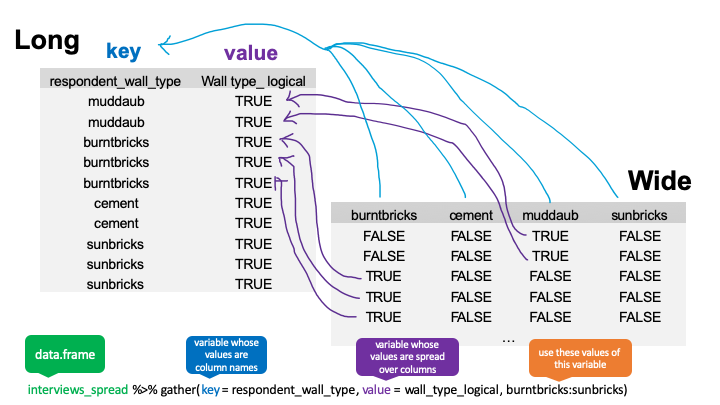
\includegraphics{./fig/wide_to_long.png}
\caption{}
\end{figure}

This creates a data frame with 524 rows (4 rows per interview
respondent). The four rows for each respondent differ only in the value
of the ``respondent\_wall\_type'' and ``dummy'' columns. View the data
to see what this looks like.

Only one row for each interview respondent is informative - we know that
if the house walls are made of ``sunbrick'' they aren't made of any
other the other materials. Therefore, we can get filter our dataset to
only keep values where \texttt{wall\_type\_logical} is \texttt{TRUE}.
Because, \texttt{wall\_type\_logical} is already either \texttt{TRUE} or
\texttt{FALSE}, when passing the column name to \texttt{filter()}, it
will automatically already only keep rows where this column has the
value \texttt{TRUE}. We can then remove the \texttt{wall\_type\_logical}
column. We do all of these steps together in the next chunk of code:

\begin{Shaded}
\begin{Highlighting}[]
\NormalTok{interviews_gather <-}\StringTok{ }\NormalTok{interviews_spread }\OperatorTok
\StringTok{    }\KeywordTok{gather}\NormalTok{(}\DataTypeTok{key =} \StringTok{"respondent_wall_type"}\NormalTok{, }\DataTypeTok{value =} \StringTok{"wall_type_logical"}\NormalTok{,}
\NormalTok{           burntbricks}\OperatorTok{:}\NormalTok{sunbricks) }\OperatorTok
\StringTok{    }\KeywordTok{filter}\NormalTok{(wall_type_logical) }\OperatorTok
\StringTok{    }\KeywordTok{select}\NormalTok{(}\OperatorTok{-}\NormalTok{wall_type_logical)}
\end{Highlighting}
\end{Shaded}

View both \texttt{interviews\_gather} and \texttt{interviews\_spread}
and compare their structure. Notice that the rows have been reordered in
\texttt{interviews\_gather} such that all of the respondents with a
particular wall type are grouped together.

\section{\texorpdfstring{Applying \texttt{spread()} to clean our
data}{Applying spread() to clean our data}}\label{applying-spread-to-clean-our-data}

Now that we've learned about \texttt{gather()} and \texttt{spread()}
we're going to put these functions to use to fix a problem with the way
that our data is structured. In the spreadsheets lesson, we learned that
it's best practice to have only a single piece of information in each
cell of your spreadsheet. In this dataset, we have several columns which
contain multiple pieces of information. For example, the
\texttt{items\_owned} column contains information about whether our
respondents owned a fridge, a television, etc. To make this data easier
to analyze, we will split this column and create a new column for each
item. Each cell in that column will either be \texttt{TRUE} or
\texttt{FALSE} and will indicate whether that interview respondent owned
that item.

\begin{Shaded}
\begin{Highlighting}[]
\NormalTok{interviews_items_owned <-}\StringTok{ }\NormalTok{interviews }\OperatorTok
\StringTok{    }\KeywordTok{separate_rows}\NormalTok{(items_owned, }\DataTypeTok{sep=}\StringTok{";"}\NormalTok{) }\OperatorTok
\StringTok{    }\KeywordTok{mutate}\NormalTok{(}\DataTypeTok{items_owned_logical =} \OtherTok{TRUE}\NormalTok{) }\OperatorTok
\StringTok{    }\KeywordTok{spread}\NormalTok{(}\DataTypeTok{key =}\NormalTok{ items_owned, }\DataTypeTok{value =}\NormalTok{ items_owned_logical, }\DataTypeTok{fill =} \OtherTok{FALSE}\NormalTok{)}

\KeywordTok{nrow}\NormalTok{(interviews_items_owned)}
\end{Highlighting}
\end{Shaded}

\begin{verbatim}
## [1] 131
\end{verbatim}

There are a couple of new concepts in this code chunk. Let's walk
through it line by line. First we create a new object
(\texttt{interviews\_items\_owned}) based on the \texttt{interviews}
dataframe.

\begin{Shaded}
\begin{Highlighting}[]
\NormalTok{interviews_items_owned <-}\StringTok{ }\NormalTok{interviews }\OperatorTok
\end{Highlighting}
\end{Shaded}

Then we use the new function \texttt{separate\_rows()} to split the
column \texttt{items\_owned} based on the presence of semi-colons
(\texttt{;}). This creates a long format version of the dataset. In this
long format version, there are 131 rows (one row for each unique item
for each respondent).

\begin{Shaded}
\begin{Highlighting}[]
\KeywordTok{separate_rows}\NormalTok{(items_owned, }\DataTypeTok{sep=}\StringTok{";"}\NormalTok{) }\OperatorTok
\end{Highlighting}
\end{Shaded}

Lastly, we use \texttt{spread()} to switch from long format to wide
format. This creates a new column for each of the unique values in the
\texttt{split\_items} column and fills those columns with \texttt{TRUE}
or \texttt{FALSE}.

\begin{Shaded}
\begin{Highlighting}[]
\KeywordTok{mutate}\NormalTok{(}\DataTypeTok{items_owned_logical =} \OtherTok{TRUE}\NormalTok{) }\OperatorTok
\StringTok{    }\KeywordTok{spread}\NormalTok{(}\DataTypeTok{key =}\NormalTok{ items_owned, }\DataTypeTok{value =}\NormalTok{ items_owned_logical, }\DataTypeTok{fill =} \OtherTok{FALSE}\NormalTok{)}
\end{Highlighting}
\end{Shaded}

View the \texttt{interviews\_items\_owned} data frame. It should have
\texttt{r\ nrow(interviews)} rows (the same number of rows you had
originally), but extra columns for each item.

You may notice that the last column in called
\texttt{\textbackslash{}}`\texttt{.\ This\ is\ because\ the\ respondents\ did\ not\ own\ any\ of\ the\ items\ that\ was\ in\ the\ interviewer\textquotesingle{}s\ list.\ We\ can\ use\ the}rename()`
function to change this name to something more meaningful:

\begin{Shaded}
\begin{Highlighting}[]
\NormalTok{interviews_items_owned <-}\StringTok{ }\NormalTok{interviews_items_owned }\OperatorTok
\StringTok{    }\KeywordTok{rename}\NormalTok{(}\DataTypeTok{no_listed_items =} \StringTok{`}\DataTypeTok{<NA>}\StringTok{`}\NormalTok{)}
\end{Highlighting}
\end{Shaded}

This format of the data allows us to do interesting things, like make a
table showing the number of respondents in each village who owned a
particular item:

\begin{Shaded}
\begin{Highlighting}[]
\NormalTok{interviews_items_owned }\OperatorTok
\StringTok{    }\KeywordTok{filter}\NormalTok{(bicycle) }\OperatorTok
\StringTok{    }\KeywordTok{group_by}\NormalTok{(village) }\OperatorTok
\StringTok{    }\KeywordTok{count}\NormalTok{(bicycle)}
\end{Highlighting}
\end{Shaded}

\begin{verbatim}
## # A tibble: 3 x 3
## # Groups:   village [3]
##   village  bicycle     n
##   <chr>    <lgl>   <int>
## 1 Chirodzo TRUE       17
## 2 God      TRUE       23
## 3 Ruaca    TRUE       20
\end{verbatim}

Or calculate the average number of items from the list owned by
respondents in each village:

\begin{Shaded}
\begin{Highlighting}[]
\NormalTok{interviews_items_owned }\OperatorTok
\StringTok{    }\KeywordTok{mutate}\NormalTok{(}\DataTypeTok{number_items =} \KeywordTok{rowSums}\NormalTok{(}\KeywordTok{select}\NormalTok{(., bicycle}\OperatorTok{:}\NormalTok{television))) }\OperatorTok
\StringTok{    }\KeywordTok{group_by}\NormalTok{(village) }\OperatorTok
\StringTok{    }\KeywordTok{summarize}\NormalTok{(}\DataTypeTok{mean_items =} \KeywordTok{mean}\NormalTok{(number_items))}
\end{Highlighting}
\end{Shaded}

\begin{verbatim}
## # A tibble: 3 x 2
##   village  mean_items
##   <chr>         <dbl>
## 1 Chirodzo       4.54
## 2 God            3.98
## 3 Ruaca          5.57
\end{verbatim}

\begin{quote}
\section{Exercise}\label{exercise-10}

\begin{enumerate}
\def\labelenumi{\arabic{enumi}.}
\tightlist
\item
  Create a new data frame (named
  \texttt{interviews\_months\_lack\_food}) that has one column for each
  month and records \texttt{TRUE} or \texttt{FALSE} for whether each
  interview respondent was lacking food in that month.
\end{enumerate}

\begin{quote}
\section{Solution}\label{solution-11}

\begin{Shaded}
\begin{Highlighting}[]
\NormalTok{interviews_months_lack_food <-}\StringTok{ }\NormalTok{interviews }\OperatorTok
\StringTok{  }\KeywordTok{separate_rows}\NormalTok{(months_lack_food, }\DataTypeTok{sep=}\StringTok{";"}\NormalTok{) }\OperatorTok
\StringTok{  }\KeywordTok{mutate}\NormalTok{(}\DataTypeTok{months_lack_food_logical  =} \OtherTok{TRUE}\NormalTok{) }\OperatorTok
\StringTok{  }\KeywordTok{spread}\NormalTok{(}\DataTypeTok{key =}\NormalTok{ months_lack_food, }\DataTypeTok{value =}\NormalTok{ months_lack_food_logical, }\DataTypeTok{fill =} \OtherTok{FALSE}\NormalTok{)}
\end{Highlighting}
\end{Shaded}
\end{quote}
\end{quote}

\begin{quote}
\begin{enumerate}
\def\labelenumi{\arabic{enumi}.}
\setcounter{enumi}{1}
\tightlist
\item
  How many months (on average) were respondents without food if they did
  belong to an irrigation association? What about if they didn't?
\end{enumerate}

\begin{quote}
\section{Solution}\label{solution-12}

\begin{Shaded}
\begin{Highlighting}[]
\NormalTok{interviews_months_lack_food }\OperatorTok
\StringTok{  }\KeywordTok{mutate}\NormalTok{(}\DataTypeTok{number_months =} \KeywordTok{rowSums}\NormalTok{(}\KeywordTok{select}\NormalTok{(., Apr}\OperatorTok{:}\NormalTok{Sept))) }\OperatorTok
\StringTok{  }\KeywordTok{group_by}\NormalTok{(memb_assoc) }\OperatorTok
\StringTok{  }\KeywordTok{summarize}\NormalTok{(}\DataTypeTok{mean_months =} \KeywordTok{mean}\NormalTok{(number_months))}
\end{Highlighting}
\end{Shaded}

\begin{verbatim}
## # A tibble: 3 x 2
##   memb_assoc mean_months
##   <chr>            <dbl>
## 1 no                2.31
## 2 yes               2.64
## 3 <NA>              2.95
\end{verbatim}
\end{quote}
\end{quote}

\section{Exporting data}\label{exporting-data}

Now that you have learned how to use \textbf{\texttt{dplyr}} to extract
information from or summarize your raw data, you may want to export
these new data sets to share them with your collaborators or for
archival.

Similar to the \texttt{read\_csv()} function used for reading CSV files
into R, there is a \texttt{write\_csv()} function that generates CSV
files from data frames.

Before using \texttt{write\_csv()}, we are going to create a new folder,
\texttt{data\_output}, in our working directory that will store this
generated dataset. We don't want to write generated datasets in the same
directory as our raw data. It's good practice to keep them separate. The
\texttt{data} folder should only contain the raw, unaltered data, and
should be left alone to make sure we don't delete or modify it. In
contrast, our script will generate the contents of the
\texttt{data\_output} directory, so even if the files it contains are
deleted, we can always re-generate them.

In preparation for our next lesson on plotting, we are going to create a
version of the dataset where each of the columns includes only one data
value. To do this, we will use spread to expand the
\texttt{months\_lack\_food} and \texttt{items\_owned} columns. We will
also create a couple of summary columns.

\begin{Shaded}
\begin{Highlighting}[]
\NormalTok{interviews_plotting <-}\StringTok{ }\NormalTok{interviews }\OperatorTok
\StringTok{    }\NormalTok{## spread data by items_owned}
\StringTok{    }\KeywordTok{separate_rows}\NormalTok{(items_owned, }\DataTypeTok{sep=}\StringTok{";"}\NormalTok{) }\OperatorTok
\StringTok{    }\KeywordTok{mutate}\NormalTok{(}\DataTypeTok{items_owned_logical =} \OtherTok{TRUE}\NormalTok{) }\OperatorTok
\StringTok{    }\KeywordTok{spread}\NormalTok{(}\DataTypeTok{key =}\NormalTok{ items_owned, }\DataTypeTok{value =}\NormalTok{ items_owned_logical, }\DataTypeTok{fill =} \OtherTok{FALSE}\NormalTok{) }\OperatorTok
\StringTok{    }\KeywordTok{rename}\NormalTok{(}\DataTypeTok{no_listed_items =} \StringTok{`}\DataTypeTok{<NA>}\StringTok{`}\NormalTok{) }\OperatorTok
\StringTok{    }\NormalTok{## spread data by months_lack_food}
\StringTok{    }\KeywordTok{separate_rows}\NormalTok{(months_lack_food, }\DataTypeTok{sep=}\StringTok{";"}\NormalTok{) }\OperatorTok
\StringTok{    }\KeywordTok{mutate}\NormalTok{(}\DataTypeTok{months_lack_food_logical =} \OtherTok{TRUE}\NormalTok{) }\OperatorTok
\StringTok{    }\KeywordTok{spread}\NormalTok{(}\DataTypeTok{key =}\NormalTok{ months_lack_food, }\DataTypeTok{value =}\NormalTok{ months_lack_food_logical, }\DataTypeTok{fill =} \OtherTok{FALSE}\NormalTok{) }\OperatorTok
\StringTok{    }\NormalTok{## add some summary columns}
\StringTok{    }\KeywordTok{mutate}\NormalTok{(}\DataTypeTok{number_months_lack_food =} \KeywordTok{rowSums}\NormalTok{(}\KeywordTok{select}\NormalTok{(., Apr}\OperatorTok{:}\NormalTok{Sept))) }\OperatorTok
\StringTok{    }\KeywordTok{mutate}\NormalTok{(}\DataTypeTok{number_items =} \KeywordTok{rowSums}\NormalTok{(}\KeywordTok{select}\NormalTok{(., bicycle}\OperatorTok{:}\NormalTok{television)))}
\end{Highlighting}
\end{Shaded}

Now we can save this data frame to our \texttt{data\_output} directory.

\begin{Shaded}
\begin{Highlighting}[]
\KeywordTok{write_csv}\NormalTok{(interviews_plotting, }\DataTypeTok{path =} \StringTok{"data_output/interviews_plotting.csv"}\NormalTok{)}
\end{Highlighting}
\end{Shaded}

\chapter{\texorpdfstring{Data Visualization with
\texttt{ggplot2}}{Data Visualization with ggplot2}}\label{ggplot}

teaching: 80\\
exercises: 35\\
adapted from:
\url{https://datacarpentry.org/r-socialsci/04-ggplot2/index.html}

questions:

\begin{itemize}
\tightlist
\item
  What are the components of a ggplot?\\
\item
  How do I create scatterplots, boxplots, and barplots?\\
\item
  How can I change the aesthetics (ex. colour, transparency) of my
  plot?\\
\item
  How can I create multiple plots at once?
\end{itemize}

objectives:

\begin{itemize}
\tightlist
\item
  Produce scatter plots, boxplots, and time series plots using ggplot.\\
\item
  Set universal plot settings.\\
\item
  Describe what faceting is and apply faceting in ggplot.\\
\item
  Modify the aesthetics of an existing ggplot plot (including axis
  labels and color).\\
\item
  Build complex and customized plots from data in a data frame.
\end{itemize}

keypoints:

\begin{itemize}
\tightlist
\item
  \texttt{ggplot2} is a flexible and useful tool for creating plots in
  R.\\
\item
  The data set and coordinate system can be defined using the
  \texttt{ggplot} function.\\
\item
  Additional layers, including geoms, are added using the \texttt{+}
  operator.\\
\item
  Boxplots are useful for visualizing the distribution of a continuous
  variable.\\
\item
  Barplot are useful for visualizing categorical data.\\
\item
  Faceting allows you to generate multiple plots based on a categorical
  variable.
\end{itemize}

We start by loading the required package. \textbf{\texttt{ggplot2}} is
also included in the \textbf{\texttt{tidyverse}} package.

\begin{Shaded}
\begin{Highlighting}[]
\KeywordTok{library}\NormalTok{(tidyverse)}
\end{Highlighting}
\end{Shaded}

If not still in the workspace, load the data we saved in the previous
lesson.

\begin{Shaded}
\begin{Highlighting}[]
\NormalTok{interviews_plotting <-}\StringTok{ }\KeywordTok{read_csv}\NormalTok{(}\StringTok{"data_output/interviews_plotting.csv"}\NormalTok{)}
\end{Highlighting}
\end{Shaded}

\begin{verbatim}
## Parsed with column specification:
## cols(
##   .default = col_logical(),
##   key_ID = col_double(),
##   village = col_character(),
##   interview_date = col_datetime(format = ""),
##   no_membrs = col_double(),
##   years_liv = col_double(),
##   respondent_wall_type = col_character(),
##   rooms = col_double(),
##   memb_assoc = col_character(),
##   affect_conflicts = col_character(),
##   liv_count = col_double(),
##   no_meals = col_double(),
##   instanceID = col_character(),
##   number_months_lack_food = col_double(),
##   number_items = col_double()
## )
\end{verbatim}

\begin{verbatim}
## See spec(...) for full column specifications.
\end{verbatim}

\section{\texorpdfstring{Plotting with
\textbf{\texttt{ggplot2}}}{Plotting with ggplot2}}\label{plotting-with-ggplot2}

\textbf{\texttt{ggplot2}} is a plotting package that makes it simple to
create complex plots from data stored in a data frame. It provides a
programmatic interface for specifying what variables to plot, how they
are displayed, and general visual properties. Therefore, we only need
minimal changes if the underlying data change or if we decide to change
from a bar plot to a scatterplot. This helps in creating publication
quality plots with minimal amounts of adjustments and tweaking.

\textbf{\texttt{ggplot2}} functions like data in the `long' format,
i.e., a column for every dimension, and a row for every observation.
Well-structured data will save you lots of time when making figures with
\textbf{\texttt{ggplot2}}

ggplot graphics are built step by step by adding new elements. Adding
layers in this fashion allows for extensive flexibility and
customization of plots.

To build a ggplot, we will use the following basic template that can be
used for different types of plots:

\begin{verbatim}
ggplot(data = <DATA>, mapping = aes(<MAPPINGS>)) +  <GEOM_FUNCTION>()
\end{verbatim}

\begin{itemize}
\tightlist
\item
  use the \texttt{ggplot()} function and bind the plot to a specific
  data frame using the \texttt{data} argument
\end{itemize}

\begin{Shaded}
\begin{Highlighting}[]
\KeywordTok{ggplot}\NormalTok{(}\DataTypeTok{data =}\NormalTok{ interviews_plotting)}
\end{Highlighting}
\end{Shaded}

\begin{itemize}
\tightlist
\item
  define a mapping (using the aesthetic (\texttt{aes}) function), by
  selecting the variables to be plotted and specifying how to present
  them in the graph, e.g.~as x/y positions or characteristics such as
  size, shape, color, etc.
\end{itemize}

\begin{Shaded}
\begin{Highlighting}[]
\KeywordTok{ggplot}\NormalTok{(}\DataTypeTok{data =}\NormalTok{ interviews_plotting, }\KeywordTok{aes}\NormalTok{(}\DataTypeTok{x =}\NormalTok{ no_membrs, }\DataTypeTok{y =}\NormalTok{ number_items))}
\end{Highlighting}
\end{Shaded}

\begin{itemize}
\item
  add `geoms' -- graphical representations of the data in the plot
  (points, lines, bars). \textbf{\texttt{ggplot2}} offers many different
  geoms; we will use some common ones today, including:
\item
  \texttt{geom\_point()} for scatter plots, dot plots, etc.
\item
  \texttt{geom\_boxplot()} for, well, boxplots!
\item
  \texttt{geom\_line()} for trend lines, time series, etc.
\end{itemize}

To add a geom to the plot use the \texttt{+} operator. Because we have
two continuous variables, let's use \texttt{geom\_point()} first:

\begin{Shaded}
\begin{Highlighting}[]
\KeywordTok{ggplot}\NormalTok{(}\DataTypeTok{data =}\NormalTok{ interviews_plotting, }\KeywordTok{aes}\NormalTok{(}\DataTypeTok{x =}\NormalTok{ no_membrs, }\DataTypeTok{y =}\NormalTok{ number_items)) }\OperatorTok{+}
\StringTok{    }\KeywordTok{geom_point}\NormalTok{()}
\end{Highlighting}
\end{Shaded}

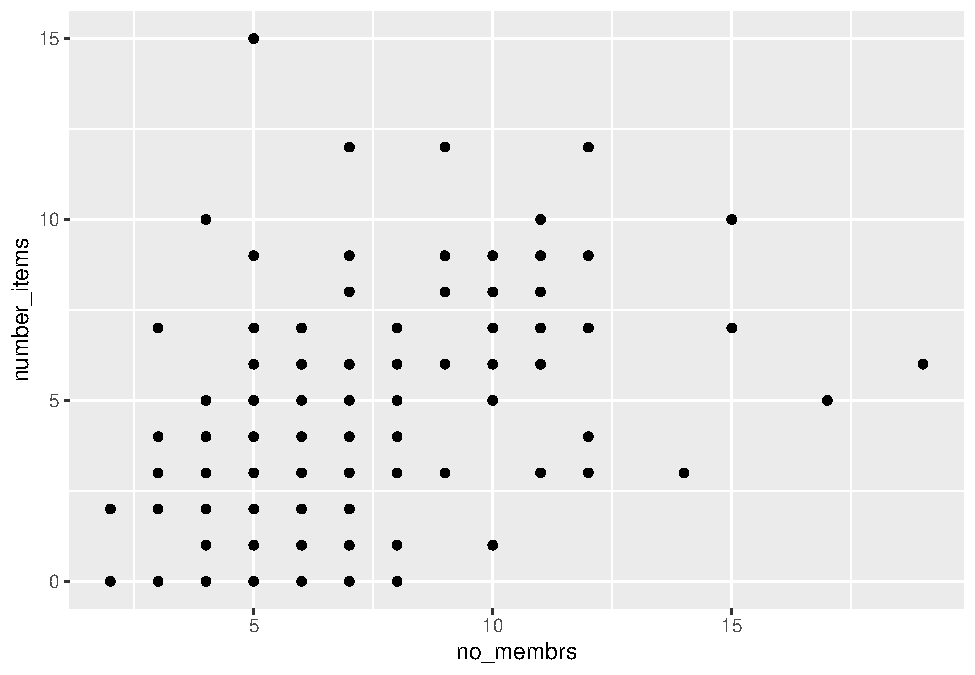
\includegraphics{2020-01-15-brynmawr_files/figure-latex/first-ggplot-1.pdf}

The \texttt{+} in the \textbf{\texttt{ggplot2}} package is particularly
useful because it allows you to modify existing \texttt{ggplot} objects.
This means you can easily set up plot templates and conveniently explore
different types of plots, so the above plot can also be generated with
code like this:

\begin{Shaded}
\begin{Highlighting}[]
\CommentTok{# Assign plot to a variable}
\NormalTok{interviews_plot <-}\StringTok{ }\KeywordTok{ggplot}\NormalTok{(}\DataTypeTok{data =}\NormalTok{ interviews_plotting, }\KeywordTok{aes}\NormalTok{(}\DataTypeTok{x =}\NormalTok{ no_membrs, }\DataTypeTok{y =}\NormalTok{ number_items))}

\CommentTok{# Draw the plot}
\NormalTok{interviews_plot }\OperatorTok{+}
\StringTok{    }\KeywordTok{geom_point}\NormalTok{()}
\end{Highlighting}
\end{Shaded}

\begin{quote}
\section{Notes}\label{notes}

\begin{itemize}
\tightlist
\item
  Anything you put in the \texttt{ggplot()} function can be seen by any
  geom layers that you add (i.e., these are universal plot settings).
  This includes the x- and y-axis mapping you set up in \texttt{aes()}.
\item
  You can also specify mappings for a given geom independently of the
  mapping defined globally in the \texttt{ggplot()} function.
\item
  The \texttt{+} sign used to add new layers must be placed at the end
  of the line containing the \emph{previous} layer. If, instead, the
  \texttt{+} sign is added at the beginning of the line containing the
  new layer, \textbf{\texttt{ggplot2}} will not add the new layer and
  will return an error message. \{: .callout\}
\end{itemize}
\end{quote}

\begin{Shaded}
\begin{Highlighting}[]
\NormalTok{## This is the correct syntax for adding layers}
\NormalTok{interviews_plot }\OperatorTok{+}
\StringTok{    }\KeywordTok{geom_point}\NormalTok{()}

\NormalTok{## This will not add the new layer and will return an error message}
\NormalTok{interviews_plot}
\OperatorTok{+}\StringTok{ }\KeywordTok{geom_point}\NormalTok{()}
\end{Highlighting}
\end{Shaded}

\section{Building your plots
iteratively}\label{building-your-plots-iteratively}

Building plots with \textbf{\texttt{ggplot2}} is typically an iterative
process. We start by defining the dataset we'll use, lay out the axes,
and choose a geom:

\begin{Shaded}
\begin{Highlighting}[]
\KeywordTok{ggplot}\NormalTok{(}\DataTypeTok{data =}\NormalTok{ interviews_plotting, }\KeywordTok{aes}\NormalTok{(}\DataTypeTok{x =}\NormalTok{ no_membrs, }\DataTypeTok{y =}\NormalTok{ number_items)) }\OperatorTok{+}
\StringTok{    }\KeywordTok{geom_point}\NormalTok{()}
\end{Highlighting}
\end{Shaded}

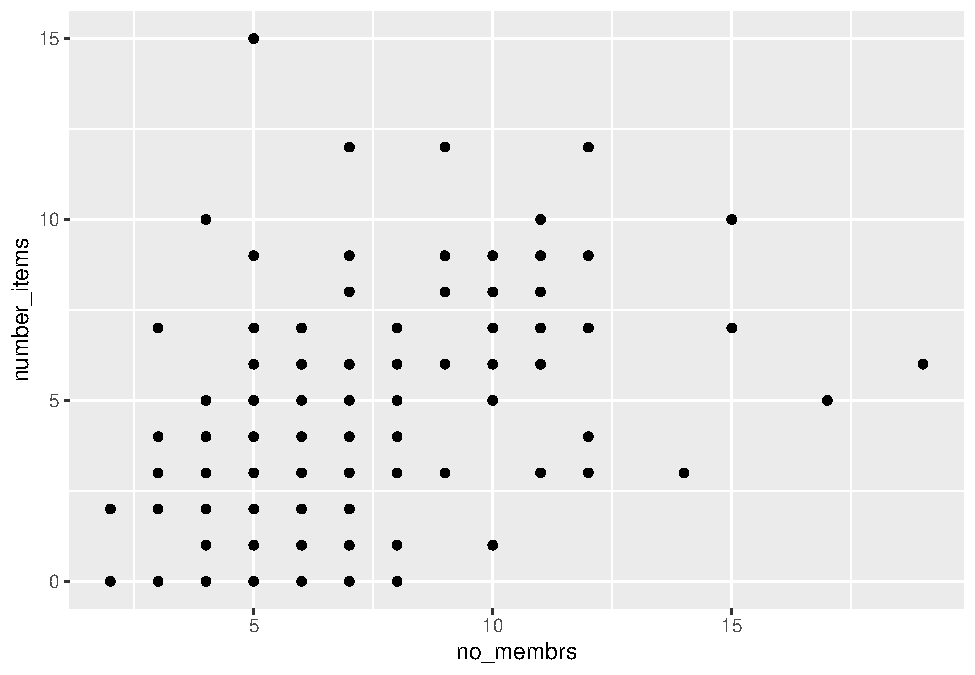
\includegraphics{2020-01-15-brynmawr_files/figure-latex/create-ggplot-object-1.pdf}

Then, we start modifying this plot to extract more information from it.
For instance, we can add transparency (\texttt{alpha}) to avoid
overplotting:

\begin{Shaded}
\begin{Highlighting}[]
\KeywordTok{ggplot}\NormalTok{(}\DataTypeTok{data =}\NormalTok{ interviews_plotting, }\KeywordTok{aes}\NormalTok{(}\DataTypeTok{x =}\NormalTok{ no_membrs, }\DataTypeTok{y =}\NormalTok{ number_items)) }\OperatorTok{+}
\StringTok{    }\KeywordTok{geom_point}\NormalTok{(}\DataTypeTok{alpha =} \FloatTok{0.5}\NormalTok{)}
\end{Highlighting}
\end{Shaded}

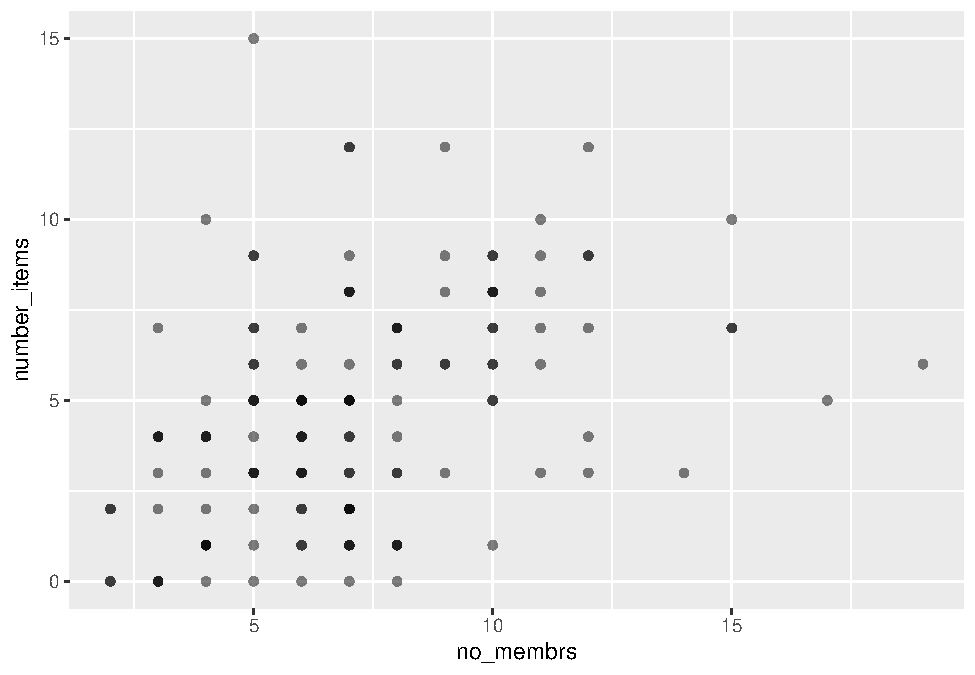
\includegraphics{2020-01-15-brynmawr_files/figure-latex/adding-transparency-1.pdf}

That only helped a little bit with the overplotting problem. We can also
introduce a little bit of randomness into the position of our points
using the \texttt{geom\_jitter()} function.

\begin{Shaded}
\begin{Highlighting}[]
\KeywordTok{ggplot}\NormalTok{(}\DataTypeTok{data =}\NormalTok{ interviews_plotting, }\KeywordTok{aes}\NormalTok{(}\DataTypeTok{x =}\NormalTok{ no_membrs, }\DataTypeTok{y =}\NormalTok{ number_items)) }\OperatorTok{+}
\StringTok{    }\KeywordTok{geom_jitter}\NormalTok{(}\DataTypeTok{alpha =} \FloatTok{0.5}\NormalTok{)}
\end{Highlighting}
\end{Shaded}

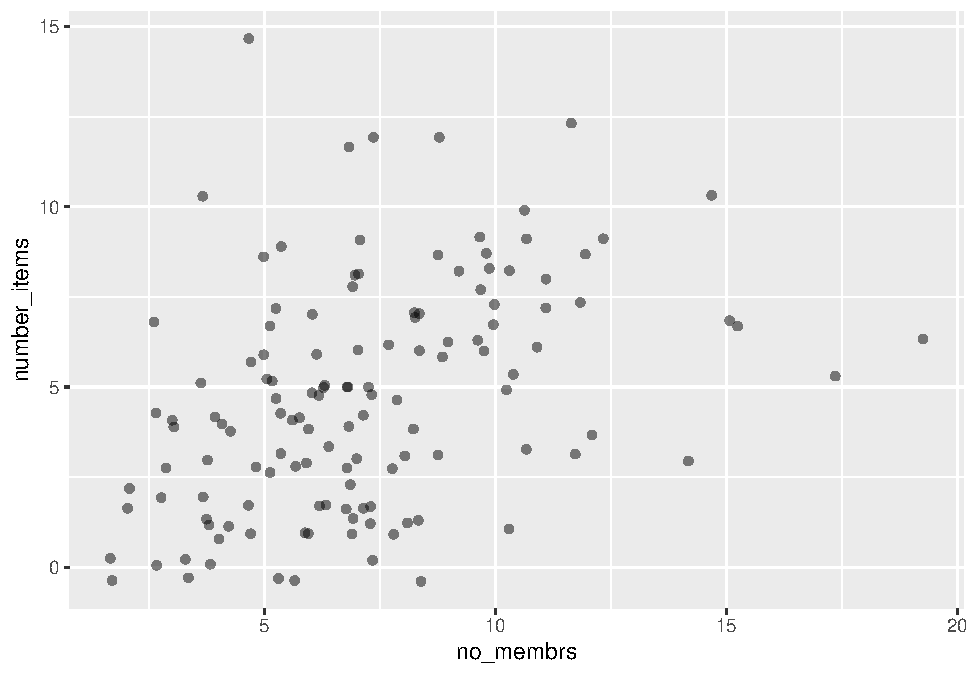
\includegraphics{2020-01-15-brynmawr_files/figure-latex/adding-jitter-1.pdf}

We can also add colors for all the points:

\begin{Shaded}
\begin{Highlighting}[]
\KeywordTok{ggplot}\NormalTok{(}\DataTypeTok{data =}\NormalTok{ interviews_plotting, }\KeywordTok{aes}\NormalTok{(}\DataTypeTok{x =}\NormalTok{ no_membrs, }\DataTypeTok{y =}\NormalTok{ number_items)) }\OperatorTok{+}
\StringTok{    }\KeywordTok{geom_jitter}\NormalTok{(}\DataTypeTok{alpha =} \FloatTok{0.5}\NormalTok{, }\DataTypeTok{color =} \StringTok{"blue"}\NormalTok{)}
\end{Highlighting}
\end{Shaded}

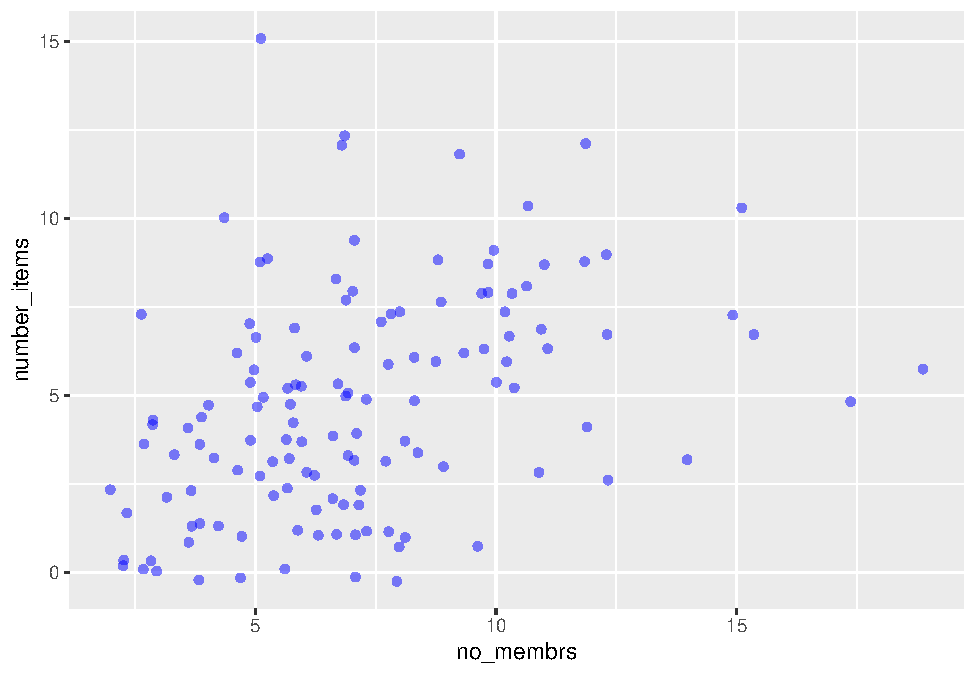
\includegraphics{2020-01-15-brynmawr_files/figure-latex/adding-colors-1.pdf}

Or to color each species in the plot differently, you could use a vector
as an input to the argument \textbf{\texttt{color}}. Because we are now
mapping features of the data to a color, instead of setting one color
for all points, the color now needs to be set inside a call to the
\textbf{\texttt{aes}} function. \textbf{\texttt{ggplot2}} will provide a
different color corresponding to different values in the vector. We set
the value of \textbf{\texttt{alpha}} outside of the
\textbf{\texttt{aes}} function call because we are using the same value
for all points. Here is an example where we color by
\textbf{\texttt{village}}:

\begin{Shaded}
\begin{Highlighting}[]
\KeywordTok{ggplot}\NormalTok{(}\DataTypeTok{data =}\NormalTok{ interviews_plotting, }\KeywordTok{aes}\NormalTok{(}\DataTypeTok{x =}\NormalTok{ no_membrs, }\DataTypeTok{y =}\NormalTok{ number_items)) }\OperatorTok{+}
\StringTok{    }\KeywordTok{geom_jitter}\NormalTok{(}\KeywordTok{aes}\NormalTok{(}\DataTypeTok{color =}\NormalTok{ village), }\DataTypeTok{alpha =} \FloatTok{0.5}\NormalTok{)}
\end{Highlighting}
\end{Shaded}

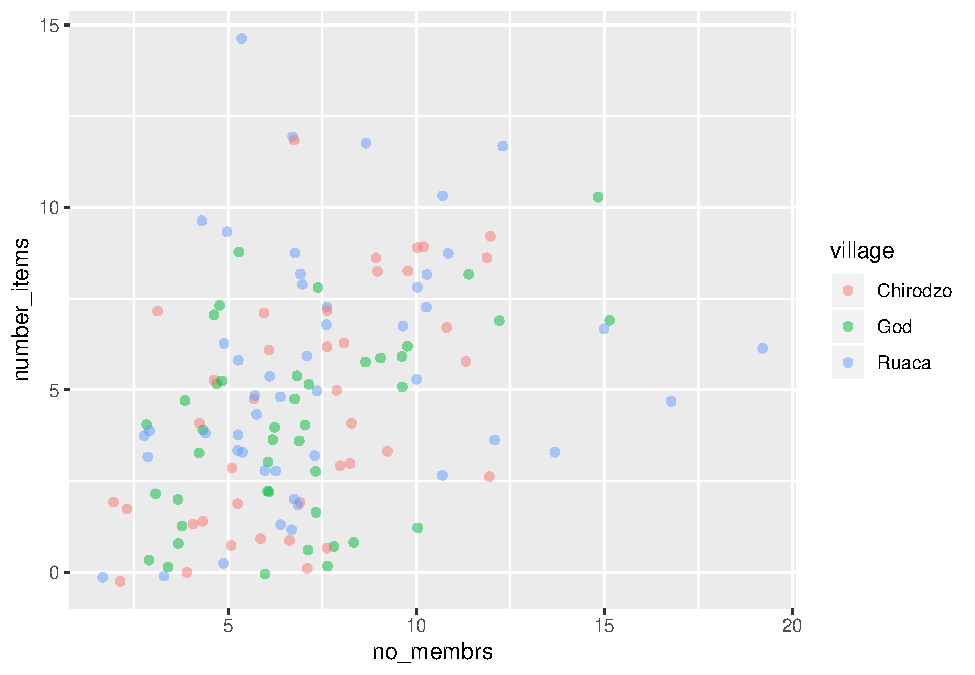
\includegraphics{2020-01-15-brynmawr_files/figure-latex/color-by-species-1.pdf}

There appears to be a positive trend between number of household members
and number of items owned (from the list provided). This trend does not
appear to be different by village.

\begin{quote}
\section{Exercise}\label{exercise-11}

Use what you just learned to create a scatter plot of \texttt{rooms} by
\texttt{village} with the \texttt{respondent\_wall\_type} showing in
different colors. Is this a good way to show this type of data?

\begin{quote}
\section{Solution}\label{solution-13}

\begin{Shaded}
\begin{Highlighting}[]
\KeywordTok{ggplot}\NormalTok{(}\DataTypeTok{data =}\NormalTok{ interviews_plotting, }\KeywordTok{aes}\NormalTok{(}\DataTypeTok{x =}\NormalTok{ village, }\DataTypeTok{y =}\NormalTok{ rooms)) }\OperatorTok{+}
\KeywordTok{geom_jitter}\NormalTok{(}\KeywordTok{aes}\NormalTok{(}\DataTypeTok{color =}\NormalTok{ respondent_wall_type))}
\end{Highlighting}
\end{Shaded}

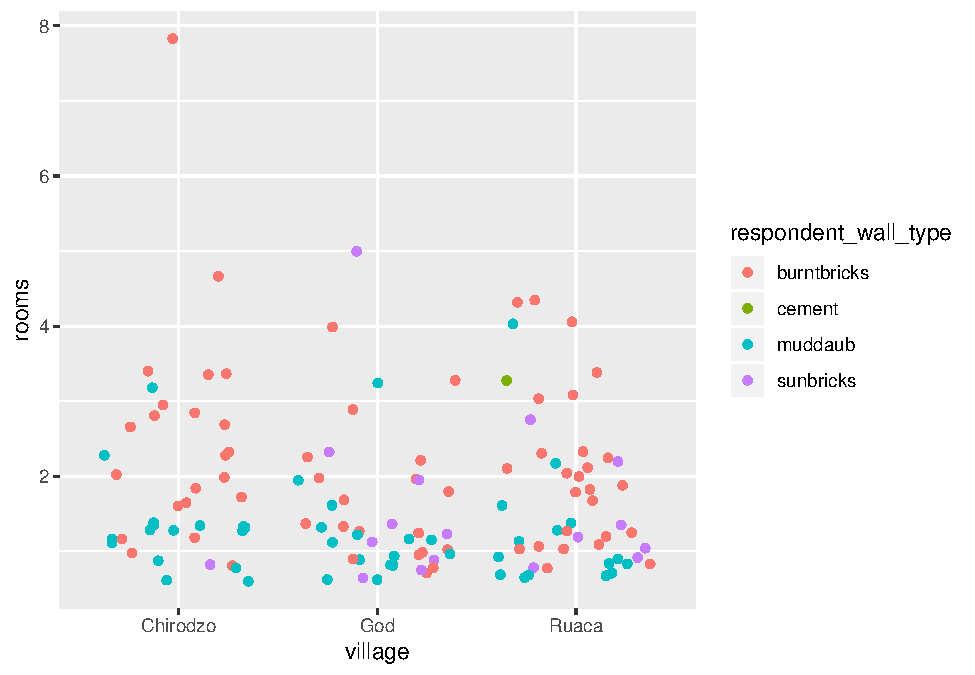
\includegraphics{2020-01-15-brynmawr_files/figure-latex/scatter-challenge-1.pdf}
This is not a good way to show this type of data because it is difficult
to distinguish between villages.
\end{quote}
\end{quote}

\section{Boxplot}\label{boxplot}

We can use boxplots to visualize the distribution of rooms for each wall
type:

\begin{Shaded}
\begin{Highlighting}[]
\KeywordTok{ggplot}\NormalTok{(}\DataTypeTok{data =}\NormalTok{ interviews_plotting, }\KeywordTok{aes}\NormalTok{(}\DataTypeTok{x =}\NormalTok{ respondent_wall_type, }\DataTypeTok{y =}\NormalTok{ rooms)) }\OperatorTok{+}
\StringTok{    }\KeywordTok{geom_boxplot}\NormalTok{()}
\end{Highlighting}
\end{Shaded}

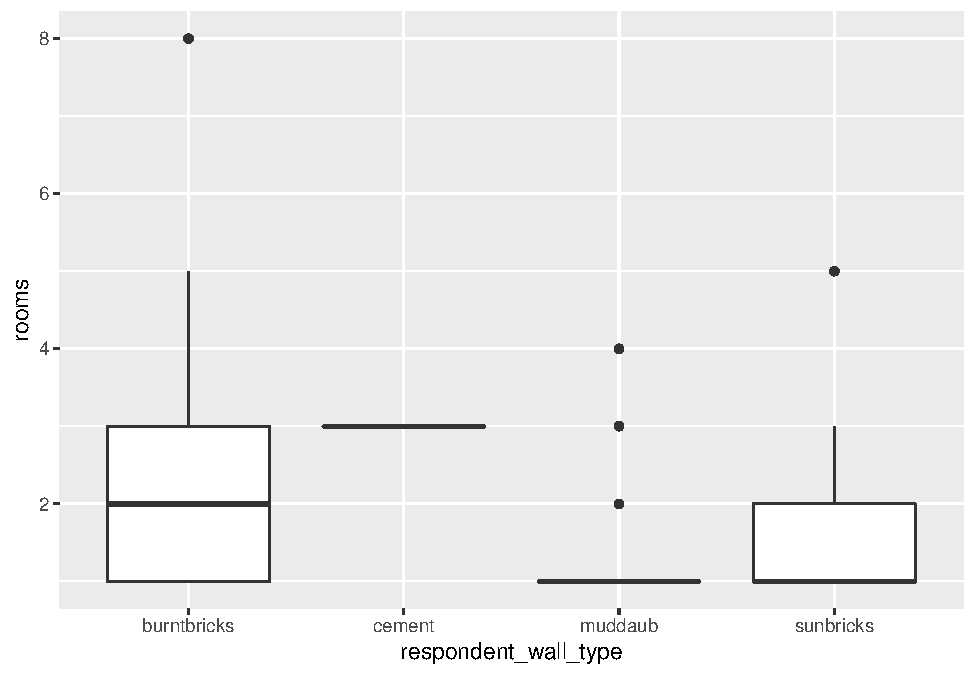
\includegraphics{2020-01-15-brynmawr_files/figure-latex/boxplot-1.pdf}

By adding points to a boxplot, we can have a better idea of the number
of measurements and of their distribution:

\begin{Shaded}
\begin{Highlighting}[]
\KeywordTok{ggplot}\NormalTok{(}\DataTypeTok{data =}\NormalTok{ interviews_plotting, }\KeywordTok{aes}\NormalTok{(}\DataTypeTok{x =}\NormalTok{ respondent_wall_type, }\DataTypeTok{y =}\NormalTok{ rooms)) }\OperatorTok{+}
\StringTok{    }\KeywordTok{geom_boxplot}\NormalTok{(}\DataTypeTok{alpha =} \DecValTok{0}\NormalTok{) }\OperatorTok{+}
\StringTok{    }\KeywordTok{geom_jitter}\NormalTok{(}\DataTypeTok{alpha =} \FloatTok{0.5}\NormalTok{, }\DataTypeTok{color =} \StringTok{"tomato"}\NormalTok{)}
\end{Highlighting}
\end{Shaded}

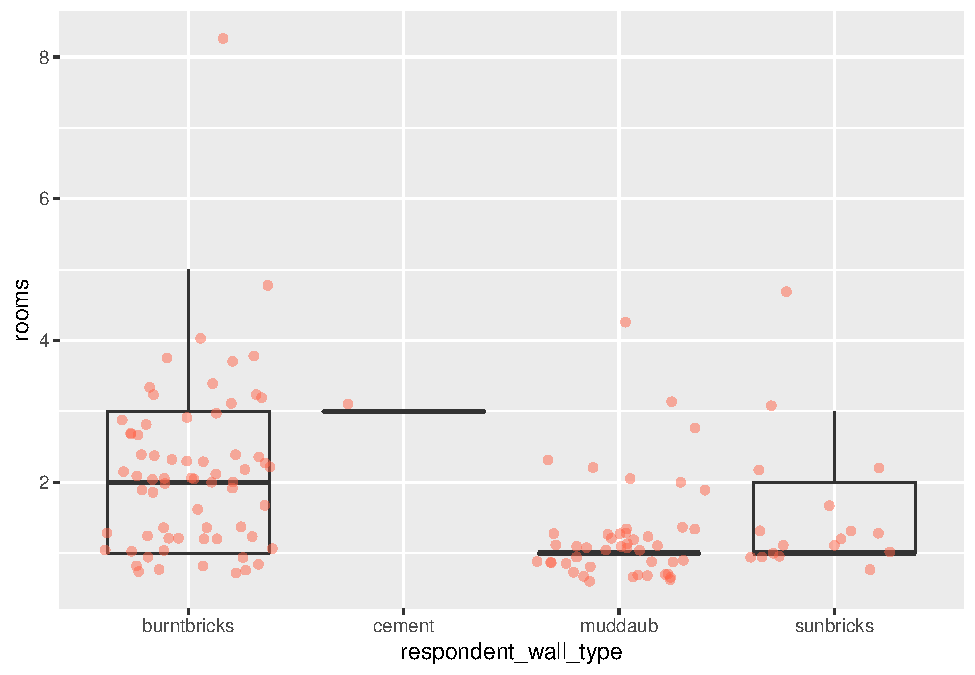
\includegraphics{2020-01-15-brynmawr_files/figure-latex/boxplot-with-points-1.pdf}

We can see that muddaub houses and sunbrick houses tend to be smaller
than burntbrick houses.

Notice how the boxplot layer is behind the jitter layer? What do you
need to change in the code to put the boxplot in front of the points
such that it's not hidden?

\begin{quote}
\section{Exercise}\label{exercise-12}

Boxplots are useful summaries, but hide the \emph{shape} of the
distribution. For example, if the distribution is bimodal, we would not
see it in a boxplot. An alternative to the boxplot is the violin plot,
where the shape (of the density of points) is drawn.

\begin{itemize}
\tightlist
\item
  Replace the box plot with a violin plot; see \texttt{geom\_violin()}.
\end{itemize}

\begin{quote}
\section{Solution}\label{solution-14}

\begin{Shaded}
\begin{Highlighting}[]
\KeywordTok{ggplot}\NormalTok{(}\DataTypeTok{data =}\NormalTok{ interviews_plotting, }\KeywordTok{aes}\NormalTok{(}\DataTypeTok{x =}\NormalTok{ respondent_wall_type, }\DataTypeTok{y =}\NormalTok{ rooms)) }\OperatorTok{+}
\StringTok{  }\KeywordTok{geom_violin}\NormalTok{(}\DataTypeTok{alpha =} \DecValTok{0}\NormalTok{) }\OperatorTok{+}
\StringTok{  }\KeywordTok{geom_jitter}\NormalTok{(}\DataTypeTok{alpha =} \FloatTok{0.5}\NormalTok{, }\DataTypeTok{color =} \StringTok{"tomato"}\NormalTok{)}
\end{Highlighting}
\end{Shaded}

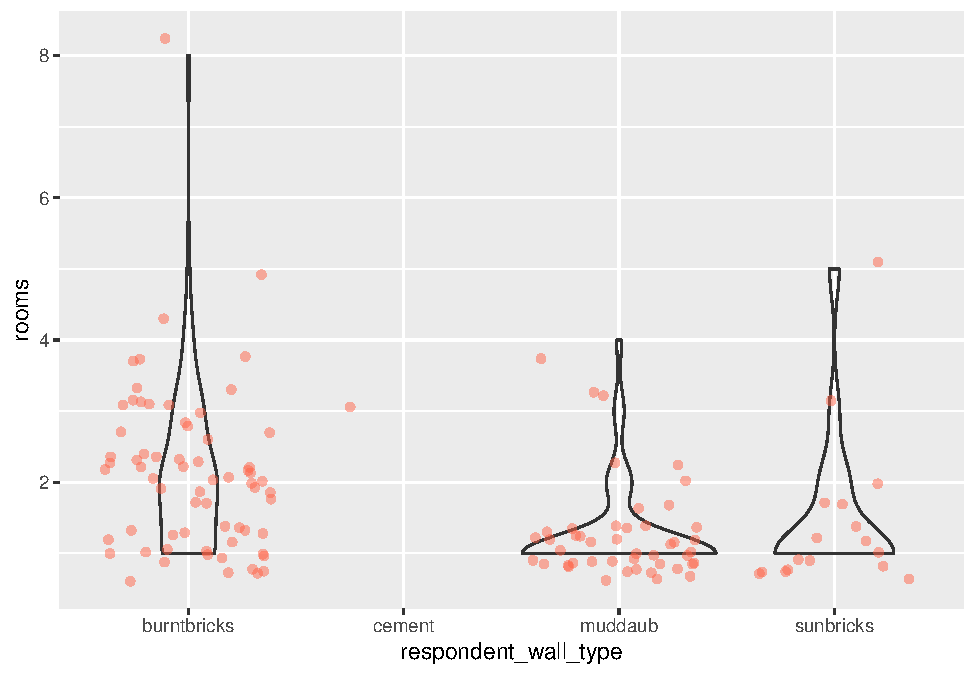
\includegraphics{2020-01-15-brynmawr_files/figure-latex/violin-plot-1.pdf}
\end{quote}

So far, we've looked at the distribution of room number within wall
type. Try making a new plot to explore the distribution of another
variable within wall type.

\begin{itemize}
\tightlist
\item
  Create a boxplot for \texttt{liv\_count} for each wall type. Overlay
  the boxplot layer on a jitter layer to show actual measurements.
\end{itemize}

\begin{quote}
\section{Solution}\label{solution-15}

\begin{Shaded}
\begin{Highlighting}[]
\KeywordTok{ggplot}\NormalTok{(}\DataTypeTok{data =}\NormalTok{ interviews_plotting, }\KeywordTok{aes}\NormalTok{(}\DataTypeTok{x =}\NormalTok{ respondent_wall_type, }\DataTypeTok{y =}\NormalTok{ liv_count)) }\OperatorTok{+}
\StringTok{  }\KeywordTok{geom_boxplot}\NormalTok{(}\DataTypeTok{alpha =} \DecValTok{0}\NormalTok{) }\OperatorTok{+}
\StringTok{  }\KeywordTok{geom_jitter}\NormalTok{(}\DataTypeTok{alpha =} \FloatTok{0.5}\NormalTok{)}
\end{Highlighting}
\end{Shaded}

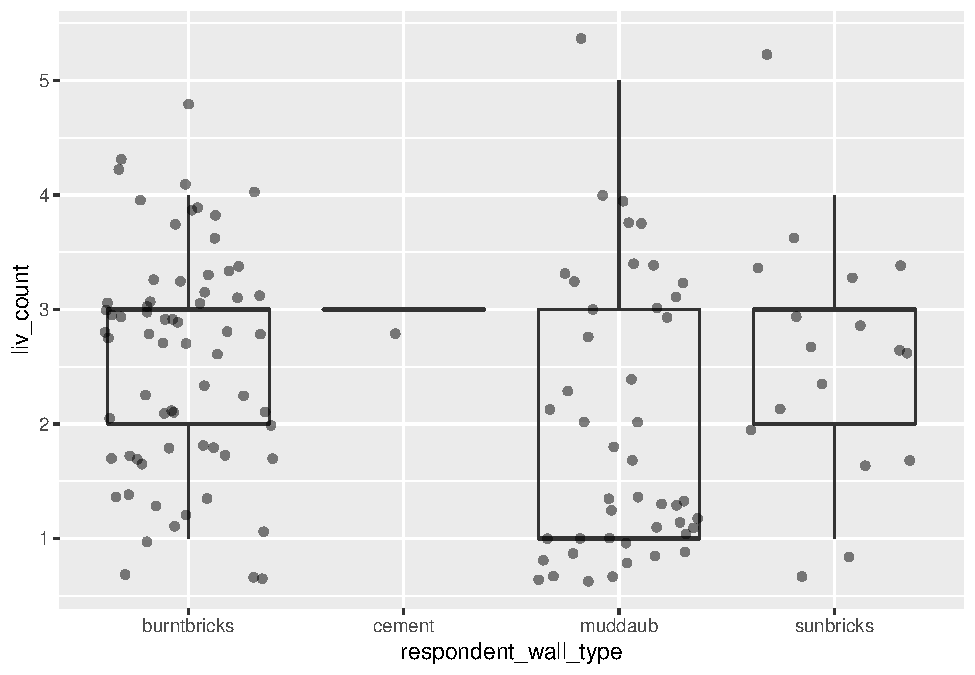
\includegraphics{2020-01-15-brynmawr_files/figure-latex/boxplot-exercise-1.pdf}
\end{quote}

\begin{itemize}
\tightlist
\item
  Add color to the data points on your boxplot according to whether the
  respondent is a member of an irrigation association
  (\texttt{memb\_assoc}).
\end{itemize}

\begin{quote}
\section{Solution}\label{solution-16}

\begin{Shaded}
\begin{Highlighting}[]
\KeywordTok{ggplot}\NormalTok{(}\DataTypeTok{data =}\NormalTok{ interviews_plotting, }\KeywordTok{aes}\NormalTok{(}\DataTypeTok{x =}\NormalTok{ respondent_wall_type, }\DataTypeTok{y =}\NormalTok{ liv_count)) }\OperatorTok{+}
\StringTok{  }\KeywordTok{geom_boxplot}\NormalTok{(}\DataTypeTok{alpha =} \DecValTok{0}\NormalTok{) }\OperatorTok{+}
\StringTok{  }\KeywordTok{geom_jitter}\NormalTok{(}\KeywordTok{aes}\NormalTok{(}\DataTypeTok{alpha =} \FloatTok{0.5}\NormalTok{, }\DataTypeTok{color =}\NormalTok{ memb_assoc))}
\end{Highlighting}
\end{Shaded}

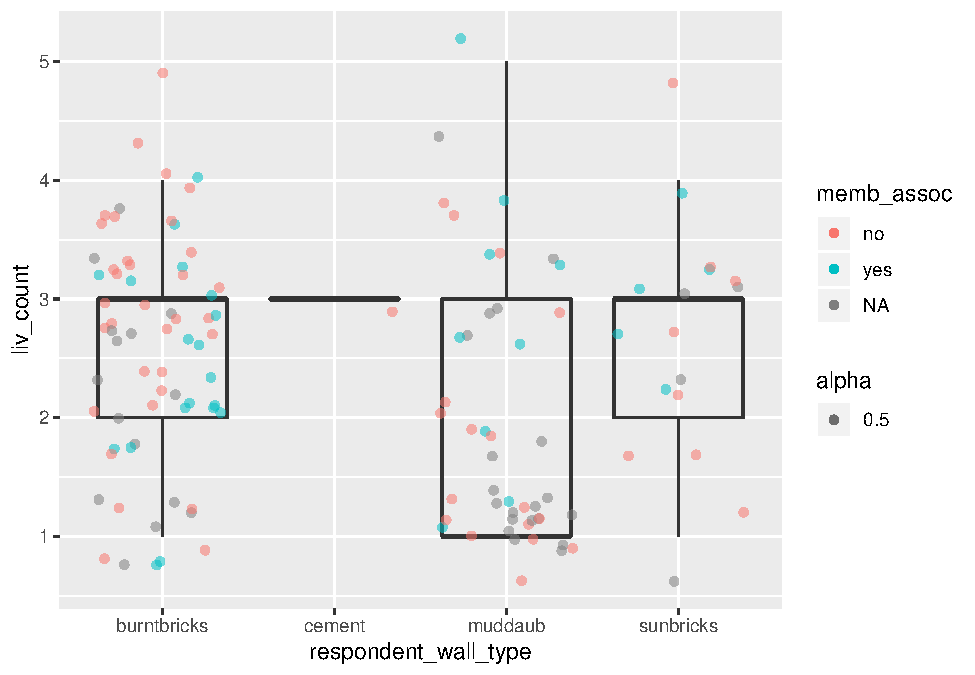
\includegraphics{2020-01-15-brynmawr_files/figure-latex/boxplot-exercise-factor-1.pdf}
\end{quote}
\end{quote}

\section{Barplots}\label{barplots}

Barplots are also useful for visualizing categorical data. By default,
\texttt{geom\_bar} accepts a variable for x, and plots the number of
instances each value of x (in this case, wall type) appears in the
dataset.

\begin{Shaded}
\begin{Highlighting}[]
\KeywordTok{ggplot}\NormalTok{(}\DataTypeTok{data =}\NormalTok{ interviews_plotting, }\KeywordTok{aes}\NormalTok{(}\DataTypeTok{x =}\NormalTok{ respondent_wall_type)) }\OperatorTok{+}
\StringTok{    }\KeywordTok{geom_bar}\NormalTok{()}
\end{Highlighting}
\end{Shaded}

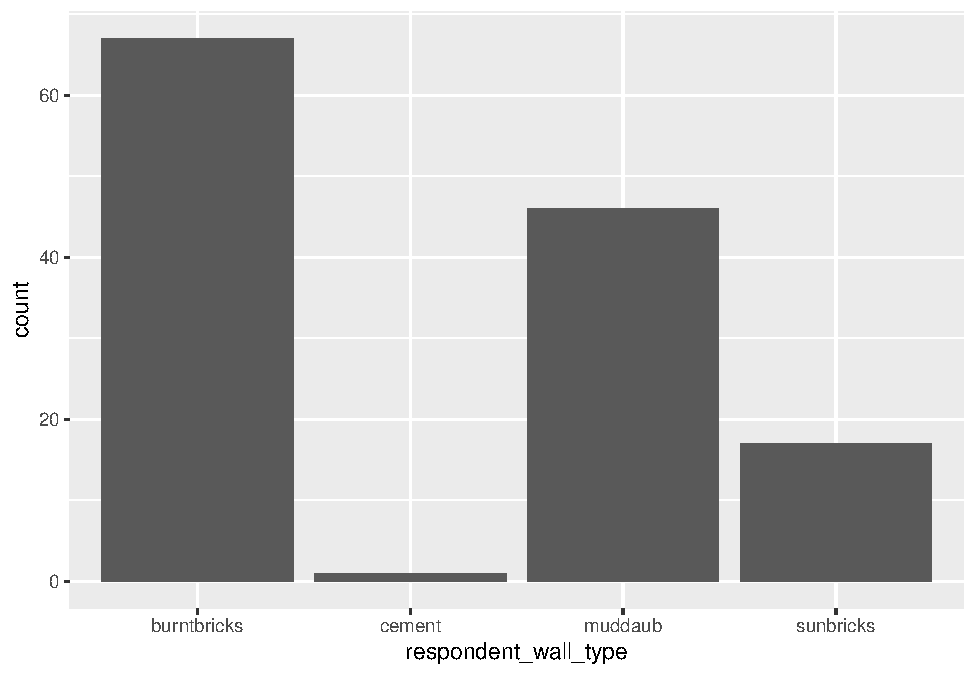
\includegraphics{2020-01-15-brynmawr_files/figure-latex/barplot-1-1.pdf}

We can use the \texttt{fill} aesthetic for the \texttt{geom\_bar()} geom
to color bars by the portion of each count that is from each village.

\begin{Shaded}
\begin{Highlighting}[]
\KeywordTok{ggplot}\NormalTok{(}\DataTypeTok{data =}\NormalTok{ interviews_plotting, }\KeywordTok{aes}\NormalTok{(}\DataTypeTok{x =}\NormalTok{ respondent_wall_type)) }\OperatorTok{+}
\StringTok{    }\KeywordTok{geom_bar}\NormalTok{(}\KeywordTok{aes}\NormalTok{(}\DataTypeTok{fill =}\NormalTok{ village))}
\end{Highlighting}
\end{Shaded}

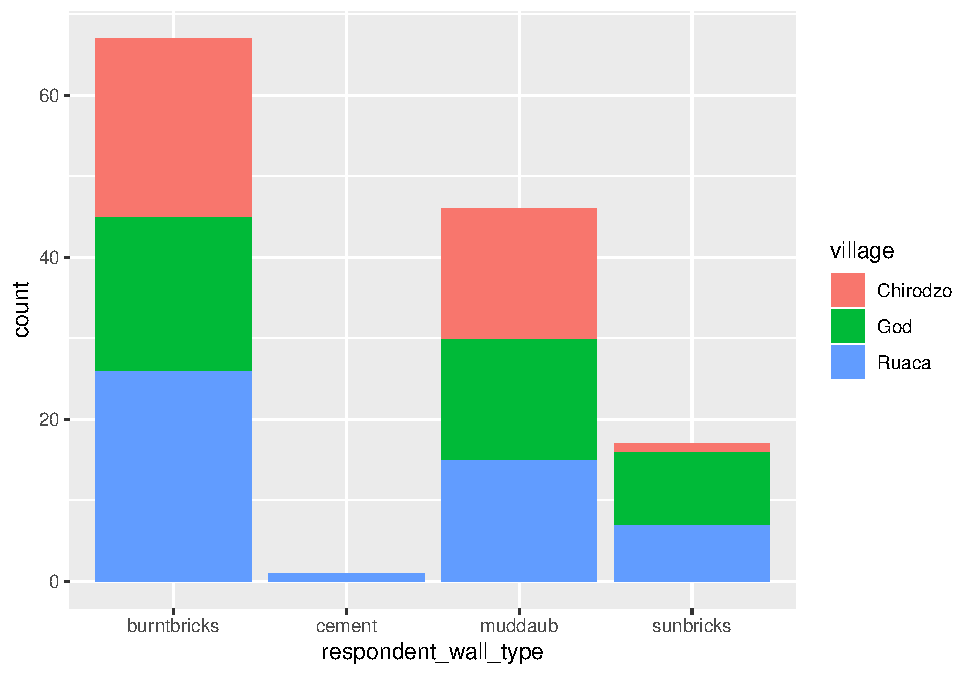
\includegraphics{2020-01-15-brynmawr_files/figure-latex/barplot-stack-1.pdf}

This creates a stacked bar chart. These are generally more difficult to
read than side-by-side bars. We can separate the portions of the stacked
bar that correspond to each village and put them side-by-side by using
the \texttt{position} argument for \texttt{geom\_bar()} and setting it
to ``dodge''.

\begin{Shaded}
\begin{Highlighting}[]
\KeywordTok{ggplot}\NormalTok{(}\DataTypeTok{data =}\NormalTok{ interviews_plotting, }\KeywordTok{aes}\NormalTok{(}\DataTypeTok{x =}\NormalTok{ respondent_wall_type)) }\OperatorTok{+}
\StringTok{    }\KeywordTok{geom_bar}\NormalTok{(}\KeywordTok{aes}\NormalTok{(}\DataTypeTok{fill =}\NormalTok{ village), }\DataTypeTok{position =} \StringTok{"dodge"}\NormalTok{)}
\end{Highlighting}
\end{Shaded}

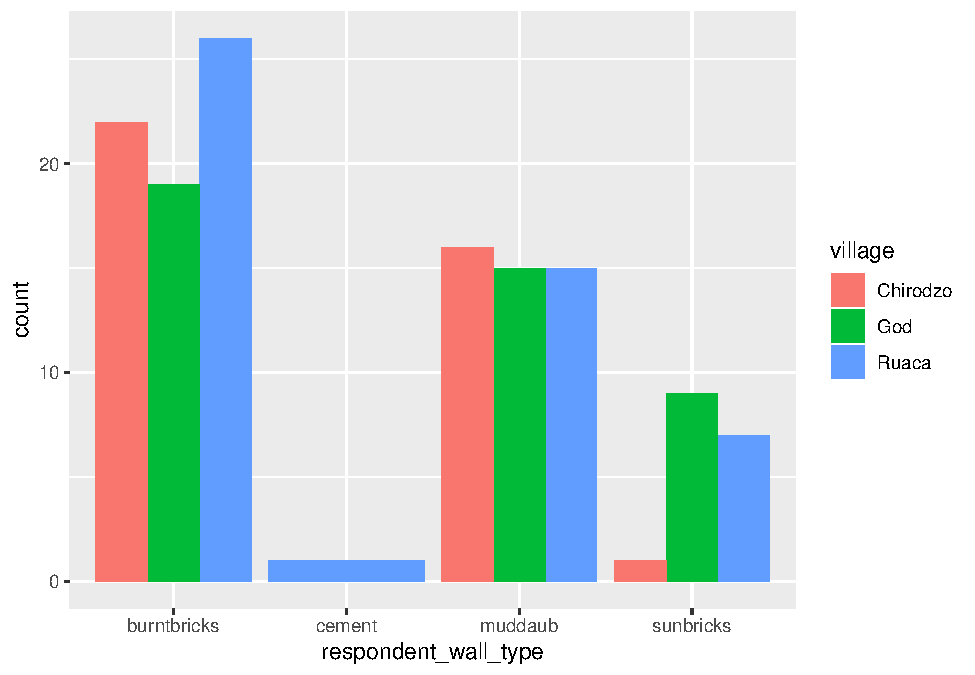
\includegraphics{2020-01-15-brynmawr_files/figure-latex/barplot-dodge-1.pdf}

This is a nicer graphic, but we're more likely to be interested in the
proportion of each housing type in each village than in the actual count
of number of houses of each type (because we might have sampled
different numbers of households in each village). To compare
proportions, we will first create a new data frame
(\texttt{percent\_wall\_type}) with a new column named ``percent''
representing the percent of each house type in each village. We will
remove houses with cement walls, as there was only one in the dataset.

\begin{Shaded}
\begin{Highlighting}[]
\NormalTok{percent_wall_type <-}\StringTok{ }\NormalTok{interviews_plotting }\OperatorTok
\StringTok{    }\KeywordTok{filter}\NormalTok{(respondent_wall_type }\OperatorTok{!=}\StringTok{ "cement"}\NormalTok{) }\OperatorTok
\StringTok{    }\KeywordTok{count}\NormalTok{(village, respondent_wall_type) }\OperatorTok
\StringTok{    }\KeywordTok{group_by}\NormalTok{(village) }\OperatorTok
\StringTok{    }\KeywordTok{mutate}\NormalTok{(}\DataTypeTok{percent =}\NormalTok{ n }\OperatorTok{/}\StringTok{ }\KeywordTok{sum}\NormalTok{(n)) }\OperatorTok
\StringTok{    }\KeywordTok{ungroup}\NormalTok{()}
\end{Highlighting}
\end{Shaded}

Now we can use this new data frame to create our plot showing the
percentage of each house type in each village.

\begin{Shaded}
\begin{Highlighting}[]
 \KeywordTok{ggplot}\NormalTok{(percent_wall_type, }\KeywordTok{aes}\NormalTok{(}\DataTypeTok{x =}\NormalTok{ village, }\DataTypeTok{y =}\NormalTok{ percent, }\DataTypeTok{fill =}\NormalTok{ respondent_wall_type)) }\OperatorTok{+}
\StringTok{     }\KeywordTok{geom_bar}\NormalTok{(}\DataTypeTok{stat =} \StringTok{"identity"}\NormalTok{, }\DataTypeTok{position =} \StringTok{"dodge"}\NormalTok{)}
\end{Highlighting}
\end{Shaded}

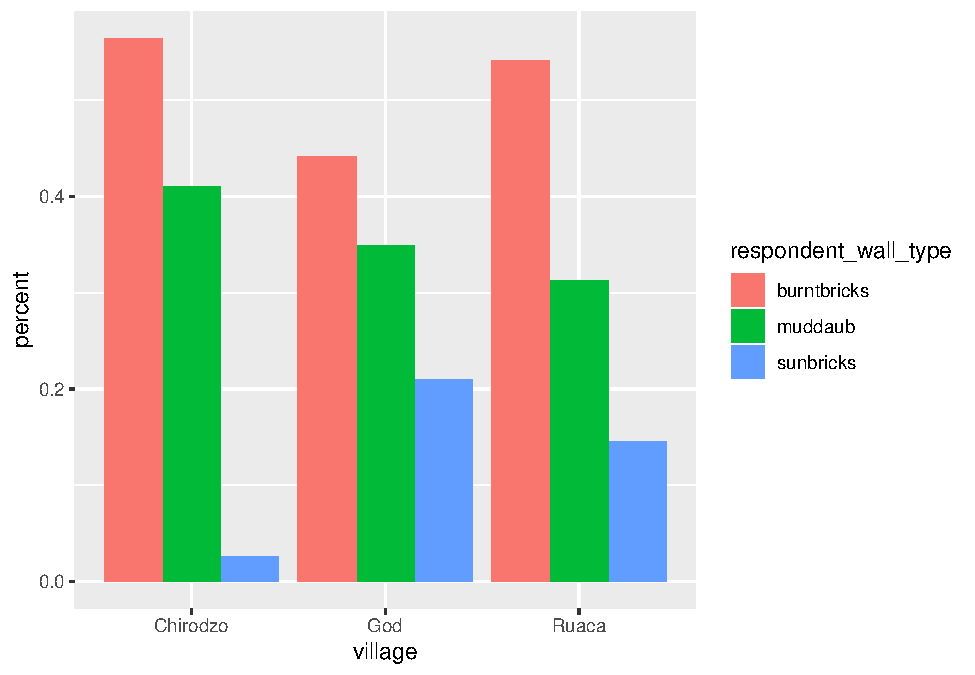
\includegraphics{2020-01-15-brynmawr_files/figure-latex/barplot-wall-type-1.pdf}

\begin{quote}
\section{Exercise}\label{exercise-13}

Create a bar plot showing the proportion of respondents in each village
who are or are not part of an irrigation association
(\texttt{memb\_assoc}). Include only respondents who answered that
question in the calculations and plot. Which village had the lowest
proportion of respondents in an irrigation association?

\begin{quote}
\section{Solution}\label{solution-17}

\begin{Shaded}
\begin{Highlighting}[]
\NormalTok{percent_memb_assoc <-}\StringTok{ }\NormalTok{interviews_plotting }\OperatorTok
\StringTok{  }\KeywordTok{filter}\NormalTok{(}\OperatorTok{!}\KeywordTok{is.na}\NormalTok{(memb_assoc)) }\OperatorTok
\StringTok{  }\KeywordTok{count}\NormalTok{(village, memb_assoc) }\OperatorTok
\StringTok{  }\KeywordTok{group_by}\NormalTok{(village) }\OperatorTok
\StringTok{  }\KeywordTok{mutate}\NormalTok{(}\DataTypeTok{percent =}\NormalTok{ n }\OperatorTok{/}\StringTok{ }\KeywordTok{sum}\NormalTok{(n)) }\OperatorTok
\StringTok{  }\KeywordTok{ungroup}\NormalTok{()}

\KeywordTok{ggplot}\NormalTok{(percent_memb_assoc, }\KeywordTok{aes}\NormalTok{(}\DataTypeTok{x =}\NormalTok{ village, }\DataTypeTok{y =}\NormalTok{ percent, }\DataTypeTok{fill =}\NormalTok{ memb_assoc)) }\OperatorTok{+}
\KeywordTok{geom_bar}\NormalTok{(}\DataTypeTok{stat =} \StringTok{"identity"}\NormalTok{, }\DataTypeTok{position =} \StringTok{"dodge"}\NormalTok{)}
\end{Highlighting}
\end{Shaded}

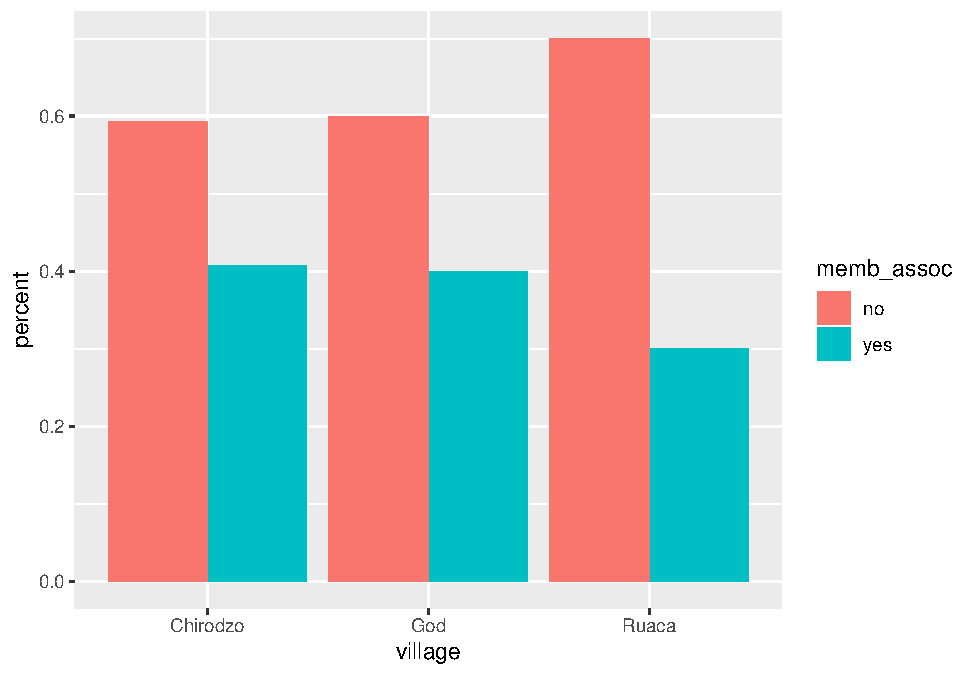
\includegraphics{2020-01-15-brynmawr_files/figure-latex/barplot-memb-assoc-1.pdf}

Ruaca had the lowest proportion of members in an irrigation association.
\end{quote}
\end{quote}

\section{Adding Labels and Titles}\label{adding-labels-and-titles}

By default, the axes labels on a plot are determined by the name of the
variable being plotted. However, \textbf{\texttt{ggplot2}} offers lots
of customization options, like specifying the axes labels, and adding a
title to the plot with relatively few lines of code. We will add more
informative x and y axis labels to our plot of proportion of house type
by village and also add a title.

\begin{Shaded}
\begin{Highlighting}[]
\KeywordTok{ggplot}\NormalTok{(percent_wall_type, }\KeywordTok{aes}\NormalTok{(}\DataTypeTok{x =}\NormalTok{ village, }\DataTypeTok{y =}\NormalTok{ percent, }\DataTypeTok{fill =}\NormalTok{ respondent_wall_type)) }\OperatorTok{+}
\StringTok{    }\KeywordTok{geom_bar}\NormalTok{(}\DataTypeTok{stat =} \StringTok{"identity"}\NormalTok{, }\DataTypeTok{position =} \StringTok{"dodge"}\NormalTok{) }\OperatorTok{+}
\StringTok{    }\KeywordTok{labs}\NormalTok{(}\DataTypeTok{title=}\StringTok{"Proportion of wall type by village"}\NormalTok{,}
         \DataTypeTok{x=}\StringTok{"Wall Type"}\NormalTok{,}
         \DataTypeTok{y=}\StringTok{"Percent"}\NormalTok{)}
\end{Highlighting}
\end{Shaded}

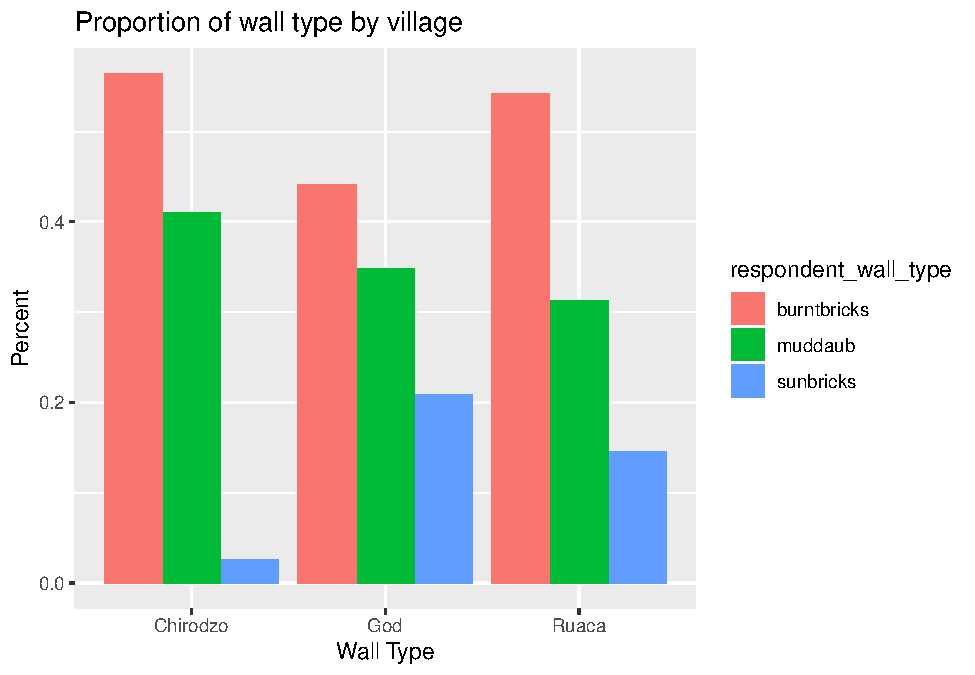
\includegraphics{2020-01-15-brynmawr_files/figure-latex/barplot-wall-types-labeled-1.pdf}

\section{Faceting}\label{faceting}

Rather than creating a single plot with side-by-side bars for each
village, we may want to create multiple plot, where each plot shows the
data for a single village. This would be especially useful if we had a
large number of villages that we had sampled, as a large number of
side-by-side bars will become more difficult to read.

\textbf{\texttt{ggplot2}} has a special technique called \emph{faceting}
that allows the user to split one plot into multiple plots based on a
factor included in the dataset. We will use it to split our barplot of
housing type proportion by village so that each village has it's own
panel in a multi-panel plot:

\begin{Shaded}
\begin{Highlighting}[]
\KeywordTok{ggplot}\NormalTok{(percent_wall_type, }\KeywordTok{aes}\NormalTok{(}\DataTypeTok{x =}\NormalTok{ respondent_wall_type, }\DataTypeTok{y =}\NormalTok{ percent)) }\OperatorTok{+}
\StringTok{    }\KeywordTok{geom_bar}\NormalTok{(}\DataTypeTok{stat =} \StringTok{"identity"}\NormalTok{, }\DataTypeTok{position =} \StringTok{"dodge"}\NormalTok{) }\OperatorTok{+}
\StringTok{    }\KeywordTok{labs}\NormalTok{(}\DataTypeTok{title=}\StringTok{"Proportion of wall type by village"}\NormalTok{,}
         \DataTypeTok{x=}\StringTok{"Wall Type"}\NormalTok{,}
         \DataTypeTok{y=}\StringTok{"Percent"}\NormalTok{) }\OperatorTok{+}
\StringTok{    }\KeywordTok{facet_wrap}\NormalTok{(}\OperatorTok{~}\StringTok{ }\NormalTok{village)}
\end{Highlighting}
\end{Shaded}

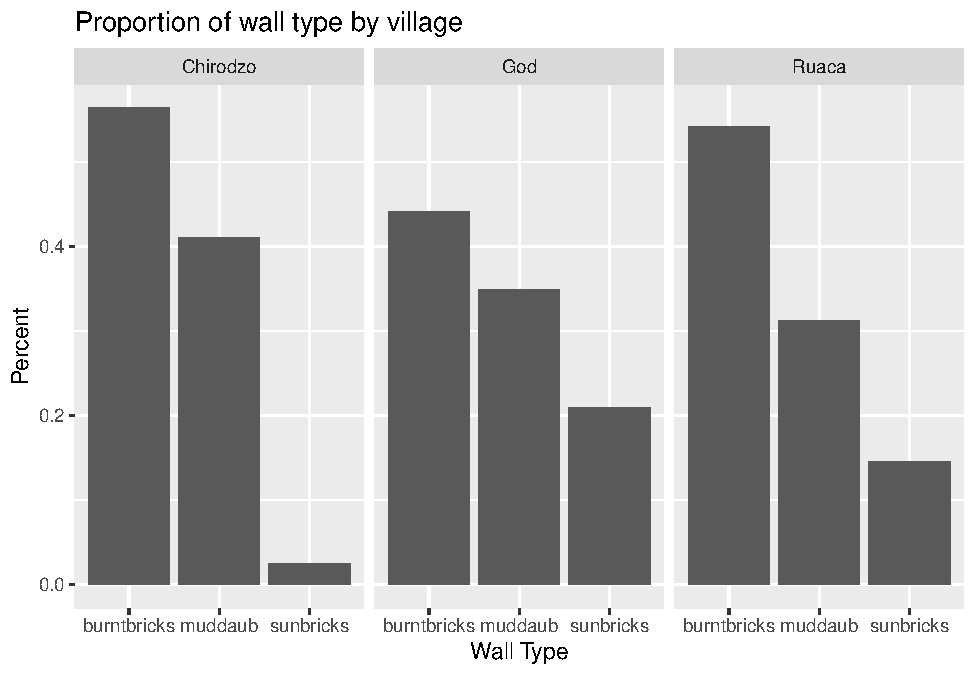
\includegraphics{2020-01-15-brynmawr_files/figure-latex/barplot-faceting-1.pdf}

Click the ``Zoom'' button in your RStudio plots pane to view a larger
version of this plot.

Usually plots with white background look more readable when printed. We
can set the background to white using the function \texttt{theme\_bw()}.
Additionally, you can remove the grid:

\begin{Shaded}
\begin{Highlighting}[]
\KeywordTok{ggplot}\NormalTok{(percent_wall_type, }\KeywordTok{aes}\NormalTok{(}\DataTypeTok{x =}\NormalTok{ respondent_wall_type, }\DataTypeTok{y =}\NormalTok{ percent)) }\OperatorTok{+}
\StringTok{    }\KeywordTok{geom_bar}\NormalTok{(}\DataTypeTok{stat =} \StringTok{"identity"}\NormalTok{, }\DataTypeTok{position =} \StringTok{"dodge"}\NormalTok{) }\OperatorTok{+}
\StringTok{    }\KeywordTok{labs}\NormalTok{(}\DataTypeTok{title=}\StringTok{"Proportion of wall type by village"}\NormalTok{,}
         \DataTypeTok{x=}\StringTok{"Wall Type"}\NormalTok{,}
         \DataTypeTok{y=}\StringTok{"Percent"}\NormalTok{) }\OperatorTok{+}
\StringTok{    }\KeywordTok{facet_wrap}\NormalTok{(}\OperatorTok{~}\StringTok{ }\NormalTok{village) }\OperatorTok{+}
\StringTok{    }\KeywordTok{theme_bw}\NormalTok{() }\OperatorTok{+}
\StringTok{    }\KeywordTok{theme}\NormalTok{(}\DataTypeTok{panel.grid =} \KeywordTok{element_blank}\NormalTok{())}
\end{Highlighting}
\end{Shaded}

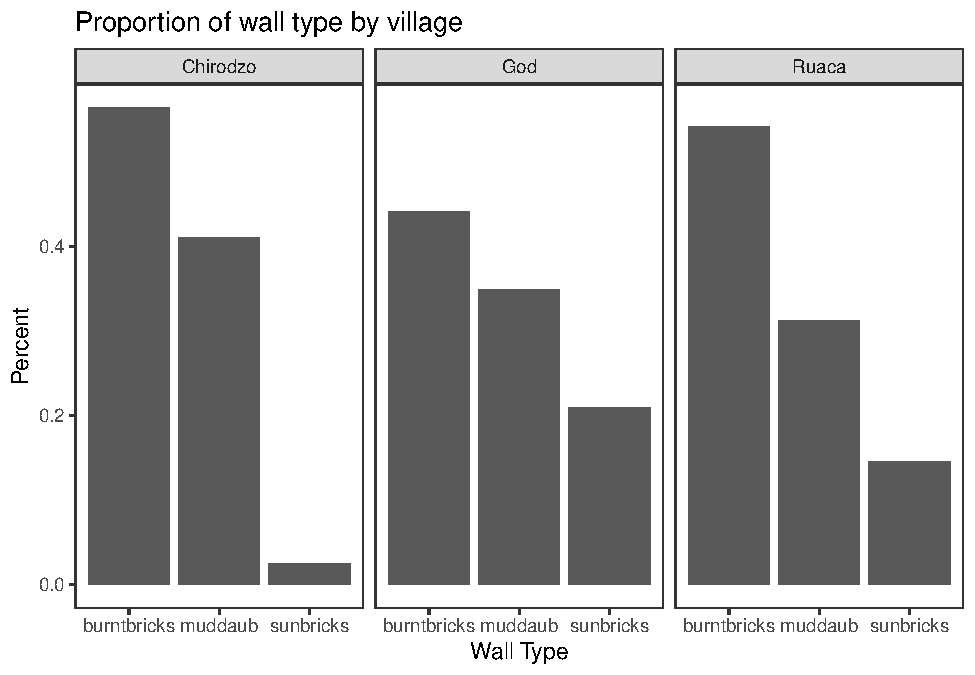
\includegraphics{2020-01-15-brynmawr_files/figure-latex/barplot-theme-bw-1.pdf}

What if we wanted to see the proportion of respondents in each village
who owned a particular item? We can calculate the percent of people in
each village who own each item and then create a faceted series of bar
plots where each plot is a particular item. First we need to calculate
the percentage of people in each village who own each item:

\begin{Shaded}
\begin{Highlighting}[]
\NormalTok{percent_items <-}\StringTok{ }\NormalTok{interviews_plotting }\OperatorTok
\StringTok{    }\KeywordTok{gather}\NormalTok{(items, items_owned_logical, bicycle}\OperatorTok{:}\NormalTok{no_listed_items) }\OperatorTok
\StringTok{    }\KeywordTok{filter}\NormalTok{(items_owned_logical) }\OperatorTok
\StringTok{    }\KeywordTok{count}\NormalTok{(items, village) }\OperatorTok
\StringTok{    }\NormalTok{## add a column with the number of people in each village}
\StringTok{    }\KeywordTok{mutate}\NormalTok{(}\DataTypeTok{people_in_village =} \KeywordTok{case_when}\NormalTok{(village }\OperatorTok{==}\StringTok{ "Chirodzo"} \OperatorTok{~}\StringTok{ }\DecValTok{39}\NormalTok{,}
\NormalTok{                                         village }\OperatorTok{==}\StringTok{ "God"} \OperatorTok{~}\StringTok{ }\DecValTok{43}\NormalTok{,}
\NormalTok{                                         village }\OperatorTok{==}\StringTok{ "Ruaca"} \OperatorTok{~}\StringTok{ }\DecValTok{49}\NormalTok{)) }\OperatorTok
\StringTok{    }\KeywordTok{mutate}\NormalTok{(}\DataTypeTok{percent =}\NormalTok{ n }\OperatorTok{/}\StringTok{ }\NormalTok{people_in_village)}
\end{Highlighting}
\end{Shaded}

To calculate this percentage data frame, we needed to use the
\texttt{case\_when()} parameter within \texttt{mutate()}. In our earlier
examples, we knew that each house was one and only one of the types
specified. However, people can (and do) own more than one item, so we
can't use the sum of the count column to give us the denominator in our
percentage calculation. Instead, we need to specify the number of
respondents in each village. Using this data frame, we can now create a
multi-paneled bar plot.

\begin{Shaded}
\begin{Highlighting}[]
\KeywordTok{ggplot}\NormalTok{(percent_items, }\KeywordTok{aes}\NormalTok{(}\DataTypeTok{x =}\NormalTok{ village, }\DataTypeTok{y =}\NormalTok{ percent)) }\OperatorTok{+}
\StringTok{    }\KeywordTok{geom_bar}\NormalTok{(}\DataTypeTok{stat =} \StringTok{"identity"}\NormalTok{, }\DataTypeTok{position =} \StringTok{"dodge"}\NormalTok{) }\OperatorTok{+}
\StringTok{    }\KeywordTok{facet_wrap}\NormalTok{(}\OperatorTok{~}\StringTok{ }\NormalTok{items) }\OperatorTok{+}
\StringTok{    }\KeywordTok{theme_bw}\NormalTok{() }\OperatorTok{+}
\StringTok{    }\KeywordTok{theme}\NormalTok{(}\DataTypeTok{panel.grid =} \KeywordTok{element_blank}\NormalTok{())}
\end{Highlighting}
\end{Shaded}

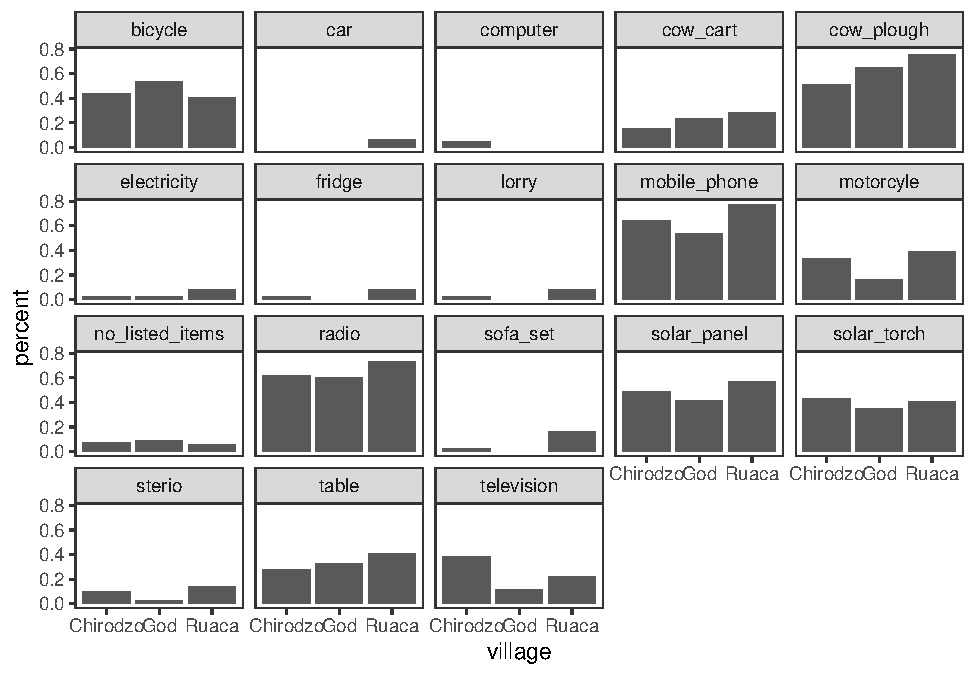
\includegraphics{2020-01-15-brynmawr_files/figure-latex/percent-items-barplot-1.pdf}

\section{\texorpdfstring{\textbf{\texttt{ggplot2}}
themes}{ggplot2 themes}}\label{ggplot2-themes}

In addition to \texttt{theme\_bw()}, which changes the plot background
to white, \textbf{\texttt{ggplot2}} comes with several other themes
which can be useful to quickly change the look of your visualization.
The complete list of themes is available at
\url{http://docs.ggplot2.org/current/ggtheme.html}.
\texttt{theme\_minimal()} and \texttt{theme\_light()} are popular, and
\texttt{theme\_void()} can be useful as a starting point to create a new
hand-crafted theme.

The
\href{https://jrnold.github.io/ggthemes/reference/index.html}{ggthemes}
package provides a wide variety of options (including an Excel 2003
theme). The
\href{https://www.ggplot2-exts.org}{\textbf{\texttt{ggplot2}} extensions
website} provides a list of packages that extend the capabilities of
\textbf{\texttt{ggplot2}}, including additional themes.

\begin{quote}
\section{Exercise}\label{exercise-14}

Experiment with at least two different themes. Build the previous plot
using each of those themes. Which do you like best? \{: .challenge\}
\end{quote}

\section{Customization}\label{customization}

Take a look at the
\href{https://www.rstudio.com/wp-content/uploads/2016/11/ggplot2-cheatsheet-2.1.pdf}{\textbf{\texttt{ggplot2}}
cheat sheet}, and think of ways you could improve the plot.

Now, let's change names of axes to something more informative than
`village' and `percent' and add a title to the figure:

\begin{Shaded}
\begin{Highlighting}[]
\KeywordTok{ggplot}\NormalTok{(percent_items, }\KeywordTok{aes}\NormalTok{(}\DataTypeTok{x =}\NormalTok{ village, }\DataTypeTok{y =}\NormalTok{ percent)) }\OperatorTok{+}
\StringTok{    }\KeywordTok{geom_bar}\NormalTok{(}\DataTypeTok{stat =} \StringTok{"identity"}\NormalTok{, }\DataTypeTok{position =} \StringTok{"dodge"}\NormalTok{) }\OperatorTok{+}
\StringTok{    }\KeywordTok{facet_wrap}\NormalTok{(}\OperatorTok{~}\StringTok{ }\NormalTok{items) }\OperatorTok{+}
\StringTok{    }\KeywordTok{labs}\NormalTok{(}\DataTypeTok{title =} \StringTok{"Percent of respondents in each village who owned each item"}\NormalTok{,}
         \DataTypeTok{x =} \StringTok{"Village"}\NormalTok{,}
         \DataTypeTok{y =} \StringTok{"Percent of Respondents"}\NormalTok{) }\OperatorTok{+}
\StringTok{    }\KeywordTok{theme_bw}\NormalTok{()}
\end{Highlighting}
\end{Shaded}

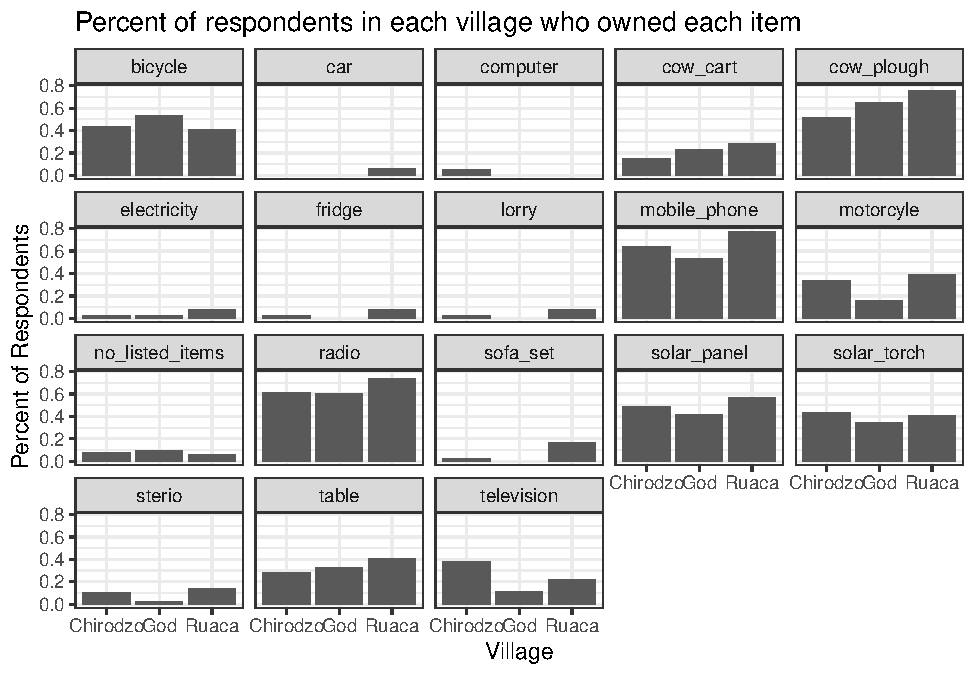
\includegraphics{2020-01-15-brynmawr_files/figure-latex/ggplot-customization-1.pdf}

The axes have more informative names, but their readability can be
improved by increasing the font size:

\begin{Shaded}
\begin{Highlighting}[]
\KeywordTok{ggplot}\NormalTok{(percent_items, }\KeywordTok{aes}\NormalTok{(}\DataTypeTok{x =}\NormalTok{ village, }\DataTypeTok{y =}\NormalTok{ percent)) }\OperatorTok{+}
\StringTok{    }\KeywordTok{geom_bar}\NormalTok{(}\DataTypeTok{stat =} \StringTok{"identity"}\NormalTok{, }\DataTypeTok{position =} \StringTok{"dodge"}\NormalTok{) }\OperatorTok{+}
\StringTok{    }\KeywordTok{facet_wrap}\NormalTok{(}\OperatorTok{~}\StringTok{ }\NormalTok{items) }\OperatorTok{+}
\StringTok{    }\KeywordTok{labs}\NormalTok{(}\DataTypeTok{title =} \StringTok{"Percent of respondents in each village who owned each item"}\NormalTok{,}
         \DataTypeTok{x =} \StringTok{"Village"}\NormalTok{,}
         \DataTypeTok{y =} \StringTok{"Percent of Respondents"}\NormalTok{) }\OperatorTok{+}
\StringTok{    }\KeywordTok{theme_bw}\NormalTok{() }\OperatorTok{+}
\StringTok{    }\KeywordTok{theme}\NormalTok{(}\DataTypeTok{text=}\KeywordTok{element_text}\NormalTok{(}\DataTypeTok{size =} \DecValTok{16}\NormalTok{))}
\end{Highlighting}
\end{Shaded}

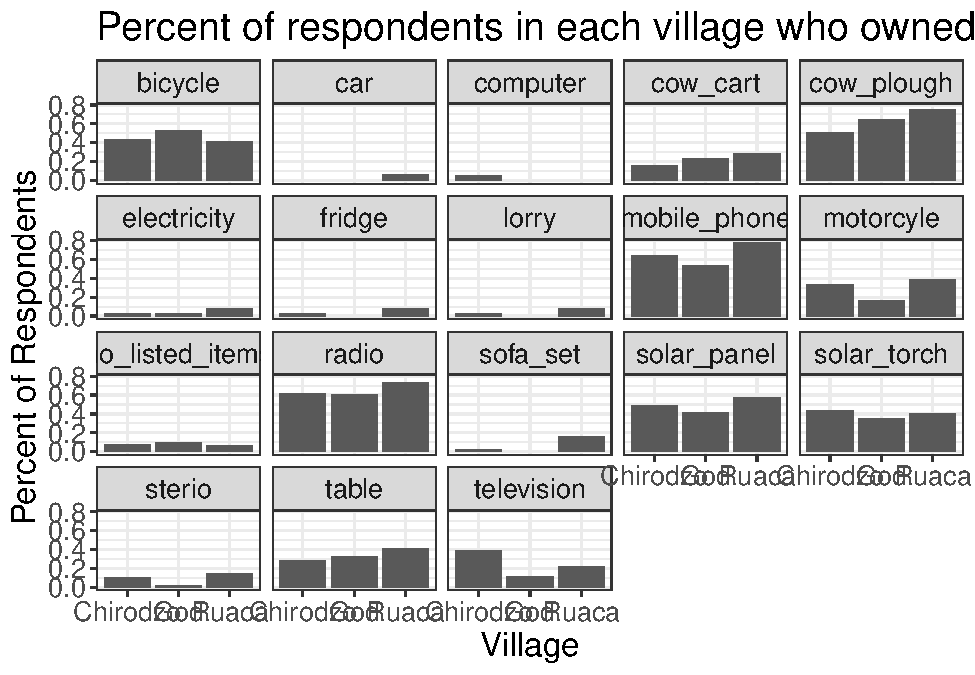
\includegraphics{2020-01-15-brynmawr_files/figure-latex/ggplot-customization-font-size-1.pdf}

Note that it is also possible to change the fonts of your plots. If you
are on Windows, you may have to install the
\href{https://github.com/wch/extrafont}{\textbf{\texttt{extrafont}}
package}, and follow the instructions included in the README for this
package.

After our manipulations, you may notice that the values on the x-axis
are still not properly readable. Let's change the orientation of the
labels and adjust them vertically and horizontally so they don't
overlap. You can use a 90-degree angle, or experiment to find the
appropriate angle for diagonally oriented labels. With a larger font,
the title also runs off. We can \texttt{\textbackslash{}n} in the string
for the title to insert a new line:

\begin{Shaded}
\begin{Highlighting}[]
\KeywordTok{ggplot}\NormalTok{(percent_items, }\KeywordTok{aes}\NormalTok{(}\DataTypeTok{x =}\NormalTok{ village, }\DataTypeTok{y =}\NormalTok{ percent)) }\OperatorTok{+}
\StringTok{    }\KeywordTok{geom_bar}\NormalTok{(}\DataTypeTok{stat =} \StringTok{"identity"}\NormalTok{, }\DataTypeTok{position =} \StringTok{"dodge"}\NormalTok{) }\OperatorTok{+}
\StringTok{    }\KeywordTok{facet_wrap}\NormalTok{(}\OperatorTok{~}\StringTok{ }\NormalTok{items) }\OperatorTok{+}
\StringTok{    }\KeywordTok{labs}\NormalTok{(}\DataTypeTok{title =} \StringTok{"Percent of respondents in each village }\CharTok{\textbackslash{}n}\StringTok{ who owned each item"}\NormalTok{,}
         \DataTypeTok{x =} \StringTok{"Village"}\NormalTok{,}
         \DataTypeTok{y =} \StringTok{"Percent of Respondents"}\NormalTok{) }\OperatorTok{+}
\StringTok{    }\KeywordTok{theme_bw}\NormalTok{() }\OperatorTok{+}
\StringTok{    }\KeywordTok{theme}\NormalTok{(}\DataTypeTok{axis.text.x =} \KeywordTok{element_text}\NormalTok{(}\DataTypeTok{colour =} \StringTok{"grey20"}\NormalTok{, }\DataTypeTok{size =} \DecValTok{12}\NormalTok{, }\DataTypeTok{angle =} \DecValTok{45}\NormalTok{, }\DataTypeTok{hjust =} \FloatTok{0.5}\NormalTok{, }\DataTypeTok{vjust =} \FloatTok{0.5}\NormalTok{),}
          \DataTypeTok{axis.text.y =} \KeywordTok{element_text}\NormalTok{(}\DataTypeTok{colour =} \StringTok{"grey20"}\NormalTok{, }\DataTypeTok{size =} \DecValTok{12}\NormalTok{),}
          \DataTypeTok{text =} \KeywordTok{element_text}\NormalTok{(}\DataTypeTok{size =} \DecValTok{16}\NormalTok{))}
\end{Highlighting}
\end{Shaded}

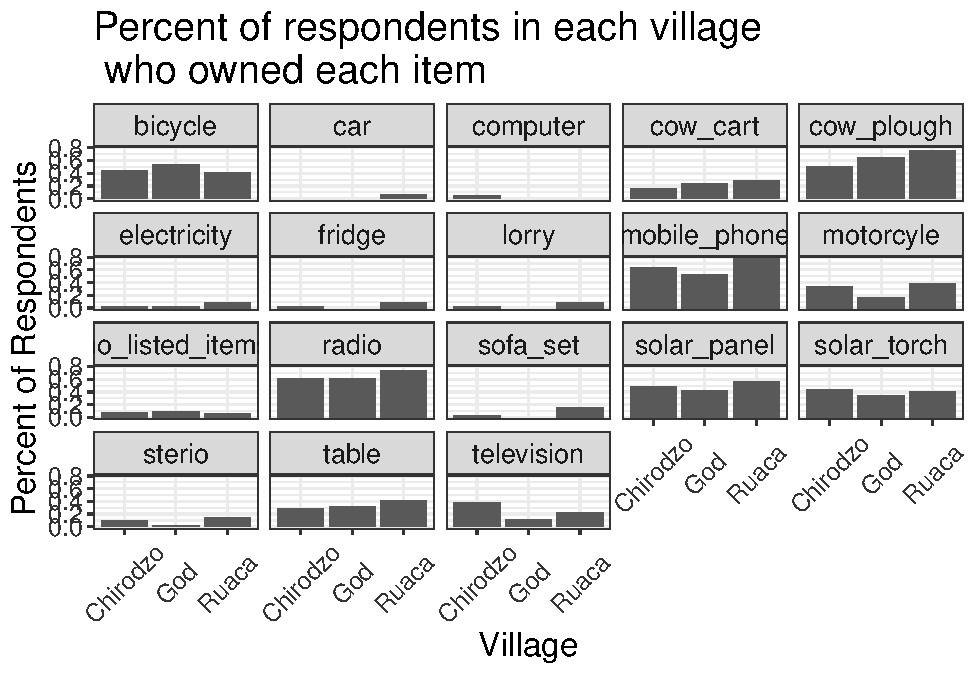
\includegraphics{2020-01-15-brynmawr_files/figure-latex/ggplot-customization-label-orientation-1.pdf}

If you like the changes you created better than the default theme, you
can save them as an object to be able to easily apply them to other
plots you may create. We can also add
\texttt{plot.title\ =\ element\_text(hjust\ =\ 0.5)} to center the
title:

\begin{Shaded}
\begin{Highlighting}[]
\NormalTok{grey_theme <-}\StringTok{ }\KeywordTok{theme}\NormalTok{(}\DataTypeTok{axis.text.x =} \KeywordTok{element_text}\NormalTok{(}\DataTypeTok{colour =} \StringTok{"grey20"}\NormalTok{, }\DataTypeTok{size =} \DecValTok{12}\NormalTok{, }\DataTypeTok{angle =} \DecValTok{45}\NormalTok{, }\DataTypeTok{hjust =} \FloatTok{0.5}\NormalTok{, }\DataTypeTok{vjust =} \FloatTok{0.5}\NormalTok{),}
                    \DataTypeTok{axis.text.y =} \KeywordTok{element_text}\NormalTok{(}\DataTypeTok{colour =} \StringTok{"grey20"}\NormalTok{, }\DataTypeTok{size =} \DecValTok{12}\NormalTok{),}
                    \DataTypeTok{text =} \KeywordTok{element_text}\NormalTok{(}\DataTypeTok{size =} \DecValTok{16}\NormalTok{),}
                    \DataTypeTok{plot.title =} \KeywordTok{element_text}\NormalTok{(}\DataTypeTok{hjust =} \FloatTok{0.5}\NormalTok{))}


\KeywordTok{ggplot}\NormalTok{(percent_items, }\KeywordTok{aes}\NormalTok{(}\DataTypeTok{x =}\NormalTok{ village, }\DataTypeTok{y =}\NormalTok{ percent)) }\OperatorTok{+}
\StringTok{    }\KeywordTok{geom_bar}\NormalTok{(}\DataTypeTok{stat =} \StringTok{"identity"}\NormalTok{, }\DataTypeTok{position =} \StringTok{"dodge"}\NormalTok{) }\OperatorTok{+}
\StringTok{    }\KeywordTok{facet_wrap}\NormalTok{(}\OperatorTok{~}\StringTok{ }\NormalTok{items) }\OperatorTok{+}
\StringTok{    }\KeywordTok{labs}\NormalTok{(}\DataTypeTok{title =} \StringTok{"Percent of respondents in each village }\CharTok{\textbackslash{}n}\StringTok{ who owned each item"}\NormalTok{,}
         \DataTypeTok{x =} \StringTok{"Village"}\NormalTok{,}
         \DataTypeTok{y =} \StringTok{"Percent of Respondents"}\NormalTok{) }\OperatorTok{+}
\StringTok{    }\NormalTok{grey_theme}
\end{Highlighting}
\end{Shaded}

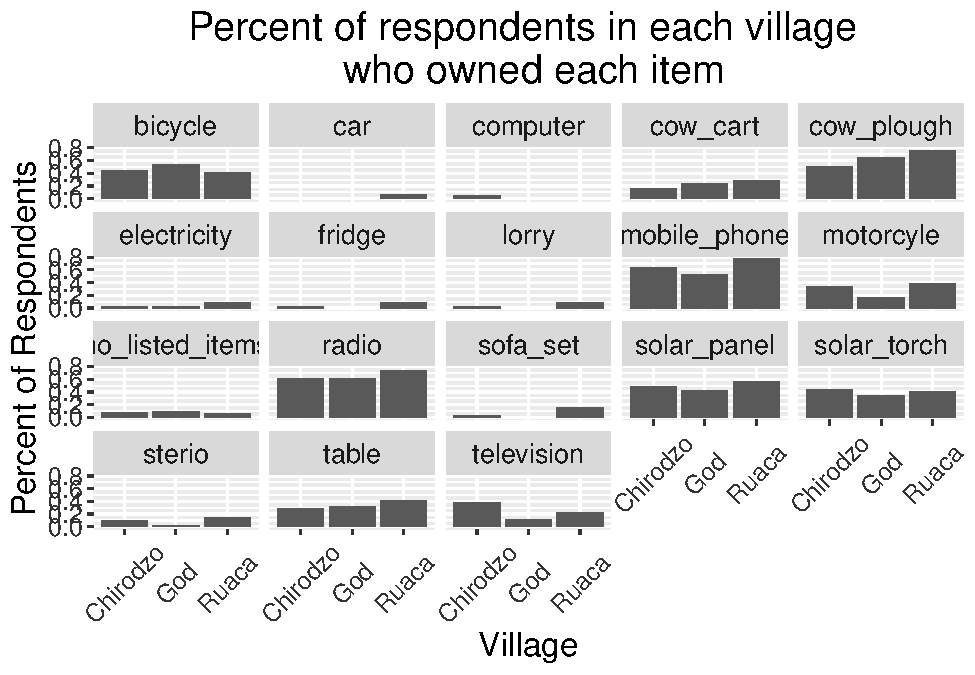
\includegraphics{2020-01-15-brynmawr_files/figure-latex/ggplot-custom-themes-1.pdf}

\begin{quote}
\section{Exercise}\label{exercise-15}

With all of this information in hand, please take another five minutes
to either improve one of the plots generated in this exercise or create
a beautiful graph of your own. Use the RStudio
\href{https://www.rstudio.com/wp-content/uploads/2016/11/ggplot2-cheatsheet-2.1.pdf}{\textbf{\texttt{ggplot2}}
cheat sheet} for inspiration. Here are some ideas:

\begin{itemize}
\tightlist
\item
  See if you can make the bars white with black outline.
\item
  Try using a different color palette (see
  \url{http://www.cookbook-r.com/Graphs/Colors_(ggplot2)/}). \{:
  .challenge\}
\end{itemize}
\end{quote}

After creating your plot, you can save it to a file in your favorite
format. The Export tab in the \textbf{Plot} pane in RStudio will save
your plots at low resolution, which will not be accepted by many
journals and will not scale well for posters.

Instead, use the \texttt{ggsave()} function, which allows you easily
change the dimension and resolution of your plot by adjusting the
appropriate arguments (\texttt{width}, \texttt{height} and
\texttt{dpi}).

Make sure you have the \texttt{fig\_output/} folder in your working
directory.

\begin{Shaded}
\begin{Highlighting}[]
\NormalTok{my_plot <-}\StringTok{ }\KeywordTok{ggplot}\NormalTok{(percent_items, }\KeywordTok{aes}\NormalTok{(}\DataTypeTok{x =}\NormalTok{ village, }\DataTypeTok{y =}\NormalTok{ percent)) }\OperatorTok{+}
\StringTok{    }\KeywordTok{geom_bar}\NormalTok{(}\DataTypeTok{stat =} \StringTok{"identity"}\NormalTok{, }\DataTypeTok{position =} \StringTok{"dodge"}\NormalTok{) }\OperatorTok{+}
\StringTok{    }\KeywordTok{facet_wrap}\NormalTok{(}\OperatorTok{~}\StringTok{ }\NormalTok{items) }\OperatorTok{+}
\StringTok{    }\KeywordTok{labs}\NormalTok{(}\DataTypeTok{title =} \StringTok{"Percent of respondents in each village }\CharTok{\textbackslash{}n}\StringTok{ who owned each item"}\NormalTok{,}
         \DataTypeTok{x =} \StringTok{"Village"}\NormalTok{,}
         \DataTypeTok{y =} \StringTok{"Percent of Respondents"}\NormalTok{) }\OperatorTok{+}
\StringTok{    }\KeywordTok{theme_bw}\NormalTok{() }\OperatorTok{+}
\StringTok{    }\KeywordTok{theme}\NormalTok{(}\DataTypeTok{axis.text.x =} \KeywordTok{element_text}\NormalTok{(}\DataTypeTok{colour =} \StringTok{"grey20"}\NormalTok{, }\DataTypeTok{size =} \DecValTok{12}\NormalTok{, }\DataTypeTok{angle =} \DecValTok{45}\NormalTok{, }\DataTypeTok{hjust =} \FloatTok{0.5}\NormalTok{, }\DataTypeTok{vjust =} \FloatTok{0.5}\NormalTok{),}
          \DataTypeTok{axis.text.y =} \KeywordTok{element_text}\NormalTok{(}\DataTypeTok{colour =} \StringTok{"grey20"}\NormalTok{, }\DataTypeTok{size =} \DecValTok{12}\NormalTok{),}
          \DataTypeTok{text =} \KeywordTok{element_text}\NormalTok{(}\DataTypeTok{size =} \DecValTok{16}\NormalTok{),}
          \DataTypeTok{plot.title =} \KeywordTok{element_text}\NormalTok{(}\DataTypeTok{hjust =} \FloatTok{0.5}\NormalTok{))}

\KeywordTok{ggsave}\NormalTok{(}\StringTok{"fig_output/name_of_file.png"}\NormalTok{, my_plot, }\DataTypeTok{width =} \DecValTok{15}\NormalTok{, }\DataTypeTok{height =} \DecValTok{10}\NormalTok{)}
\end{Highlighting}
\end{Shaded}

Note: The parameters \texttt{width} and \texttt{height} also determine
the font size in the saved plot.

\chapter{\texorpdfstring{Advanced variable creation with
\texttt{forcats}}{Advanced variable creation with forcats}}\label{forcats}

teaching: 60\\
exercises: 15\\
adapted from:\\
questions:

\begin{itemize}
\tightlist
\item
  ``How can I easily create new categorical variables?''
\end{itemize}

objectives:

\begin{itemize}
\item
\end{itemize}

keypoints:

\begin{itemize}
\item
\end{itemize}

\begin{Shaded}
\begin{Highlighting}[]
\KeywordTok{library}\NormalTok{(tidyverse)}
\NormalTok{interviews <-}\StringTok{ }\KeywordTok{read_csv}\NormalTok{(}\StringTok{"data/SAFI_clean.csv"}\NormalTok{, }\DataTypeTok{na =} \StringTok{"NULL"}\NormalTok{)}
\end{Highlighting}
\end{Shaded}

\section{Factors}\label{factors}

R has a special data class, called factor, to deal with categorical data
that you may encounter when creating plots or doing statistical
analyses. Factors are very useful and actually contribute to making R
particularly well suited to working with data. So we are going to spend
a little time introducing them.

Factors represent categorical data. They are stored as integers
associated with labels and they can be ordered or unordered. While
factors look (and often behave) like character vectors, they are
actually treated as integer vectors by R. So you need to be very careful
when treating them as strings.

Factors are particularly useful when making plots or running statistical
models. Unfortunately, they can also be very tricky to work with,
because they are secretly numbers behind the scenes. Working with
factors in base R can lead to errors that are almost impossible for
human analysts to catch, but there is a \texttt{tidyverse} package that
makes it much easier to work with factors, and prevents many common
mistakes. It is called \texttt{forcats} (an anagram of the word
``factors'' and also because it is a package \textbf{for} working with
\textbf{cat}egorical variable\textbf{s}).

Let's load the \texttt{forcats} package so we can use the functions it
comes with

\begin{Shaded}
\begin{Highlighting}[]
\KeywordTok{library}\NormalTok{(forcats)}
\end{Highlighting}
\end{Shaded}

Once created, factors can only contain a pre-defined set of values,
known as \emph{levels}. By default, base R always sorts levels in
alphabetical order. For instance, if you have a factor with 2 levels:

\begin{Shaded}
\begin{Highlighting}[]
\KeywordTok{factor}\NormalTok{(}\KeywordTok{c}\NormalTok{(}\StringTok{"earth"}\NormalTok{, }\StringTok{"cement"}\NormalTok{, }\StringTok{"cement"}\NormalTok{, }\StringTok{"earth"}\NormalTok{))}
\end{Highlighting}
\end{Shaded}

\begin{verbatim}
## [1] earth  cement cement earth 
## Levels: cement earth
\end{verbatim}

R will assign \texttt{1} to the level \texttt{"cement"} and \texttt{2}
to the level \texttt{"earth"} (because \texttt{c} comes before
\texttt{e} in the alphabet, even though the first element in this vector
is\texttt{"earth"}).

In R's memory, factors are represented by integers (1, 2), but are more
informative than integers because factors are self describing:
\texttt{"cement"}, \texttt{"earth"} is more descriptive than \texttt{1},
and \texttt{2}. Which one is ``earth''? You wouldn't be able to tell
just from the integer data. Factors, on the other hand, have this
information built in. It is particularly helpful when there are many
levels.

However, the default ordering of levels in base R is less than ideal,
because it depends on the language you have set for your R session, and
can lead to un-reproducble code.

In the \texttt{forcats} package, there is a function that makes a factor
but creates the levels in the order they appear.

\begin{Shaded}
\begin{Highlighting}[]
\NormalTok{respondent_floor_type <-}\StringTok{ }\KeywordTok{as_factor}\NormalTok{(}\KeywordTok{c}\NormalTok{(}\StringTok{"earth"}\NormalTok{, }\StringTok{"cement"}\NormalTok{, }\StringTok{"cement"}\NormalTok{, }\StringTok{"earth"}\NormalTok{))}
\NormalTok{respondent_floor_type}
\end{Highlighting}
\end{Shaded}

\begin{verbatim}
## [1] earth  cement cement earth 
## Levels: earth cement
\end{verbatim}

You can see the levels and their order by using the function
\texttt{levels()} and you can find the number of levels using
\texttt{nlevels()}:

\begin{Shaded}
\begin{Highlighting}[]
\KeywordTok{levels}\NormalTok{(respondent_floor_type)}
\end{Highlighting}
\end{Shaded}

\begin{verbatim}
## [1] "earth"  "cement"
\end{verbatim}

\begin{Shaded}
\begin{Highlighting}[]
\KeywordTok{nlevels}\NormalTok{(respondent_floor_type)}
\end{Highlighting}
\end{Shaded}

\begin{verbatim}
## [1] 2
\end{verbatim}

\section{reordering factor levels}\label{reordering-factor-levels}

Sometimes, the order of the factors does not matter, other times you
might want to specify the order because it is meaningful (e.g., ``low'',
``medium'', ``high''), it improves your visualization, or it is required
by a particular type of analysis. In \texttt{forcats}, one way to
reorder our levels in the \texttt{respondent\_floor\_type} vector would
be:

\begin{Shaded}
\begin{Highlighting}[]
\NormalTok{respondent_floor_type }\CommentTok{# current order}
\end{Highlighting}
\end{Shaded}

\begin{verbatim}
## [1] earth  cement cement earth 
## Levels: earth cement
\end{verbatim}

\begin{Shaded}
\begin{Highlighting}[]
\NormalTok{respondent_floor_type <-}\StringTok{ }\KeywordTok{fct_relevel}\NormalTok{(respondent_floor_type, }\StringTok{"cement"}\NormalTok{, }\StringTok{"earth"}\NormalTok{)}
\NormalTok{respondent_floor_type }\CommentTok{# after re-ordering}
\end{Highlighting}
\end{Shaded}

\begin{verbatim}
## [1] earth  cement cement earth 
## Levels: cement earth
\end{verbatim}

This is perhaps easier to see with a few more factor levels. Let's use
our real data,

\begin{Shaded}
\begin{Highlighting}[]
\NormalTok{respondent_floor_type <-}\StringTok{ }\KeywordTok{as_factor}\NormalTok{(interviews}\OperatorTok{$}\NormalTok{respondent_wall_type)}
\KeywordTok{levels}\NormalTok{(respondent_floor_type)}
\end{Highlighting}
\end{Shaded}

\begin{verbatim}
## [1] "muddaub"     "burntbricks" "sunbricks"   "cement"
\end{verbatim}

Say we want \texttt{sunbricks} to come first in the factor order. We can
use \texttt{fct\_relevel} to move it up.

\begin{Shaded}
\begin{Highlighting}[]
\NormalTok{respondent_floor_type }\CommentTok{# current order}
\end{Highlighting}
\end{Shaded}

\begin{verbatim}
##   [1] muddaub     muddaub     burntbricks burntbricks burntbricks muddaub    
##   [7] muddaub     burntbricks burntbricks burntbricks sunbricks   burntbricks
##  [13] burntbricks burntbricks sunbricks   muddaub     sunbricks   muddaub    
##  [19] burntbricks burntbricks burntbricks muddaub     burntbricks burntbricks
##  [25] burntbricks burntbricks burntbricks muddaub     burntbricks muddaub    
##  [31] muddaub     muddaub     muddaub     burntbricks muddaub     sunbricks  
##  [37] burntbricks muddaub     muddaub     burntbricks muddaub     sunbricks  
##  [43] muddaub     muddaub     muddaub     burntbricks muddaub     muddaub    
##  [49] burntbricks muddaub     muddaub     burntbricks burntbricks muddaub    
##  [55] muddaub     burntbricks burntbricks burntbricks muddaub     burntbricks
##  [61] muddaub     muddaub     muddaub     muddaub     burntbricks burntbricks
##  [67] burntbricks burntbricks muddaub     burntbricks burntbricks burntbricks
##  [73] burntbricks burntbricks burntbricks burntbricks burntbricks sunbricks  
##  [79] muddaub     sunbricks   muddaub     muddaub     muddaub     burntbricks
##  [85] burntbricks burntbricks burntbricks muddaub     burntbricks muddaub    
##  [91] burntbricks burntbricks burntbricks sunbricks   burntbricks muddaub    
##  [97] sunbricks   burntbricks burntbricks muddaub     sunbricks   sunbricks  
## [103] sunbricks   sunbricks   sunbricks   burntbricks muddaub     burntbricks
## [109] muddaub     sunbricks   burntbricks burntbricks muddaub     burntbricks
## [115] burntbricks muddaub     sunbricks   burntbricks burntbricks muddaub    
## [121] muddaub     burntbricks burntbricks sunbricks   burntbricks burntbricks
## [127] burntbricks cement      muddaub     burntbricks burntbricks
## Levels: muddaub burntbricks sunbricks cement
\end{verbatim}

\begin{Shaded}
\begin{Highlighting}[]
\NormalTok{respondent_floor_type <-}\StringTok{ }\KeywordTok{fct_relevel}\NormalTok{(respondent_floor_type, }\StringTok{"sunbricks"}\NormalTok{)}
\NormalTok{respondent_floor_type }\CommentTok{# after re-ordering}
\end{Highlighting}
\end{Shaded}

\begin{verbatim}
##   [1] muddaub     muddaub     burntbricks burntbricks burntbricks muddaub    
##   [7] muddaub     burntbricks burntbricks burntbricks sunbricks   burntbricks
##  [13] burntbricks burntbricks sunbricks   muddaub     sunbricks   muddaub    
##  [19] burntbricks burntbricks burntbricks muddaub     burntbricks burntbricks
##  [25] burntbricks burntbricks burntbricks muddaub     burntbricks muddaub    
##  [31] muddaub     muddaub     muddaub     burntbricks muddaub     sunbricks  
##  [37] burntbricks muddaub     muddaub     burntbricks muddaub     sunbricks  
##  [43] muddaub     muddaub     muddaub     burntbricks muddaub     muddaub    
##  [49] burntbricks muddaub     muddaub     burntbricks burntbricks muddaub    
##  [55] muddaub     burntbricks burntbricks burntbricks muddaub     burntbricks
##  [61] muddaub     muddaub     muddaub     muddaub     burntbricks burntbricks
##  [67] burntbricks burntbricks muddaub     burntbricks burntbricks burntbricks
##  [73] burntbricks burntbricks burntbricks burntbricks burntbricks sunbricks  
##  [79] muddaub     sunbricks   muddaub     muddaub     muddaub     burntbricks
##  [85] burntbricks burntbricks burntbricks muddaub     burntbricks muddaub    
##  [91] burntbricks burntbricks burntbricks sunbricks   burntbricks muddaub    
##  [97] sunbricks   burntbricks burntbricks muddaub     sunbricks   sunbricks  
## [103] sunbricks   sunbricks   sunbricks   burntbricks muddaub     burntbricks
## [109] muddaub     sunbricks   burntbricks burntbricks muddaub     burntbricks
## [115] burntbricks muddaub     sunbricks   burntbricks burntbricks muddaub    
## [121] muddaub     burntbricks burntbricks sunbricks   burntbricks burntbricks
## [127] burntbricks cement      muddaub     burntbricks burntbricks
## Levels: sunbricks muddaub burntbricks cement
\end{verbatim}

The \texttt{fct\_relevel} function allows you to move any number of
levels to any location. If you re-specify the entire list of levels, it
will re-order the whole list. But, if you just specify one level (like
we did here) that level gets moved to the front of the list.

Most of the useful functions in \texttt{forcats} start with
\texttt{fct\_}, so you can try typing that much in your Console or code
chunk and hitting Tab to use the code completion feature in RStudio to
see what some of the other functions are called.

Another way to re-order your factor levels is by frequency, so the most
common factor levels come first, and the less common come later. (This
is often useful for plotting!)

\begin{Shaded}
\begin{Highlighting}[]
\KeywordTok{levels}\NormalTok{(respondent_floor_type)}
\end{Highlighting}
\end{Shaded}

\begin{verbatim}
## [1] "sunbricks"   "muddaub"     "burntbricks" "cement"
\end{verbatim}

\begin{Shaded}
\begin{Highlighting}[]
\NormalTok{respondent_floor_type <-}\StringTok{ }\KeywordTok{fct_infreq}\NormalTok{(respondent_floor_type, }\DataTypeTok{ordered =} \OtherTok{TRUE}\NormalTok{)}
\KeywordTok{levels}\NormalTok{(respondent_floor_type)}
\end{Highlighting}
\end{Shaded}

\begin{verbatim}
## [1] "burntbricks" "muddaub"     "sunbricks"   "cement"
\end{verbatim}

\section{renaming factor levels}\label{renaming-factor-levels}

\texttt{forcats} makes easy to rename factor levels. Let's say we made a
mistake and need to recode ``cement'' to ``brick''. We'd use the
\texttt{fct\_recode} function to do this.

\begin{Shaded}
\begin{Highlighting}[]
\KeywordTok{levels}\NormalTok{(respondent_floor_type)}
\end{Highlighting}
\end{Shaded}

\begin{verbatim}
## [1] "burntbricks" "muddaub"     "sunbricks"   "cement"
\end{verbatim}

\begin{Shaded}
\begin{Highlighting}[]
\NormalTok{respondent_floor_type <-}\StringTok{ }\KeywordTok{fct_recode}\NormalTok{(respondent_floor_type, }\DataTypeTok{brick =} \StringTok{"cement"}\NormalTok{)}

\KeywordTok{levels}\NormalTok{(respondent_floor_type)}
\end{Highlighting}
\end{Shaded}

\begin{verbatim}
## [1] "burntbricks" "muddaub"     "sunbricks"   "brick"
\end{verbatim}

\begin{Shaded}
\begin{Highlighting}[]
\NormalTok{respondent_floor_type}
\end{Highlighting}
\end{Shaded}

\begin{verbatim}
##   [1] muddaub     muddaub     burntbricks burntbricks burntbricks muddaub    
##   [7] muddaub     burntbricks burntbricks burntbricks sunbricks   burntbricks
##  [13] burntbricks burntbricks sunbricks   muddaub     sunbricks   muddaub    
##  [19] burntbricks burntbricks burntbricks muddaub     burntbricks burntbricks
##  [25] burntbricks burntbricks burntbricks muddaub     burntbricks muddaub    
##  [31] muddaub     muddaub     muddaub     burntbricks muddaub     sunbricks  
##  [37] burntbricks muddaub     muddaub     burntbricks muddaub     sunbricks  
##  [43] muddaub     muddaub     muddaub     burntbricks muddaub     muddaub    
##  [49] burntbricks muddaub     muddaub     burntbricks burntbricks muddaub    
##  [55] muddaub     burntbricks burntbricks burntbricks muddaub     burntbricks
##  [61] muddaub     muddaub     muddaub     muddaub     burntbricks burntbricks
##  [67] burntbricks burntbricks muddaub     burntbricks burntbricks burntbricks
##  [73] burntbricks burntbricks burntbricks burntbricks burntbricks sunbricks  
##  [79] muddaub     sunbricks   muddaub     muddaub     muddaub     burntbricks
##  [85] burntbricks burntbricks burntbricks muddaub     burntbricks muddaub    
##  [91] burntbricks burntbricks burntbricks sunbricks   burntbricks muddaub    
##  [97] sunbricks   burntbricks burntbricks muddaub     sunbricks   sunbricks  
## [103] sunbricks   sunbricks   sunbricks   burntbricks muddaub     burntbricks
## [109] muddaub     sunbricks   burntbricks burntbricks muddaub     burntbricks
## [115] burntbricks muddaub     sunbricks   burntbricks burntbricks muddaub    
## [121] muddaub     burntbricks burntbricks sunbricks   burntbricks burntbricks
## [127] burntbricks brick       muddaub     burntbricks burntbricks
## Levels: burntbricks < muddaub < sunbricks < brick
\end{verbatim}

\subsection{Converting factors}\label{converting-factors}

If you are working in the tidyverse, your data will come in with very
few factor variables by default. So, the most common conversion you will
need to do is from a character vector to a factor, like we did before,

\begin{Shaded}
\begin{Highlighting}[]
\KeywordTok{as_factor}\NormalTok{(}\KeywordTok{c}\NormalTok{(}\StringTok{"earth"}\NormalTok{, }\StringTok{"cement"}\NormalTok{, }\StringTok{"cement"}\NormalTok{, }\StringTok{"earth"}\NormalTok{))}
\end{Highlighting}
\end{Shaded}

\begin{verbatim}
## [1] earth  cement cement earth 
## Levels: earth cement
\end{verbatim}

If you find yourself with many factors you need to convert to character
vectors, it's good to check your read-in code first, to see if you
accidentally used \texttt{read.csv} instead of \texttt{read\_csv}. In
the unlikely event you need to convert a factor to a character vector,
you use \texttt{as.character(x)}.

\begin{Shaded}
\begin{Highlighting}[]
\KeywordTok{as.character}\NormalTok{(respondent_floor_type)}
\end{Highlighting}
\end{Shaded}

\begin{verbatim}
##   [1] "muddaub"     "muddaub"     "burntbricks" "burntbricks" "burntbricks"
##   [6] "muddaub"     "muddaub"     "burntbricks" "burntbricks" "burntbricks"
##  [11] "sunbricks"   "burntbricks" "burntbricks" "burntbricks" "sunbricks"  
##  [16] "muddaub"     "sunbricks"   "muddaub"     "burntbricks" "burntbricks"
##  [21] "burntbricks" "muddaub"     "burntbricks" "burntbricks" "burntbricks"
##  [26] "burntbricks" "burntbricks" "muddaub"     "burntbricks" "muddaub"    
##  [31] "muddaub"     "muddaub"     "muddaub"     "burntbricks" "muddaub"    
##  [36] "sunbricks"   "burntbricks" "muddaub"     "muddaub"     "burntbricks"
##  [41] "muddaub"     "sunbricks"   "muddaub"     "muddaub"     "muddaub"    
##  [46] "burntbricks" "muddaub"     "muddaub"     "burntbricks" "muddaub"    
##  [51] "muddaub"     "burntbricks" "burntbricks" "muddaub"     "muddaub"    
##  [56] "burntbricks" "burntbricks" "burntbricks" "muddaub"     "burntbricks"
##  [61] "muddaub"     "muddaub"     "muddaub"     "muddaub"     "burntbricks"
##  [66] "burntbricks" "burntbricks" "burntbricks" "muddaub"     "burntbricks"
##  [71] "burntbricks" "burntbricks" "burntbricks" "burntbricks" "burntbricks"
##  [76] "burntbricks" "burntbricks" "sunbricks"   "muddaub"     "sunbricks"  
##  [81] "muddaub"     "muddaub"     "muddaub"     "burntbricks" "burntbricks"
##  [86] "burntbricks" "burntbricks" "muddaub"     "burntbricks" "muddaub"    
##  [91] "burntbricks" "burntbricks" "burntbricks" "sunbricks"   "burntbricks"
##  [96] "muddaub"     "sunbricks"   "burntbricks" "burntbricks" "muddaub"    
## [101] "sunbricks"   "sunbricks"   "sunbricks"   "sunbricks"   "sunbricks"  
## [106] "burntbricks" "muddaub"     "burntbricks" "muddaub"     "sunbricks"  
## [111] "burntbricks" "burntbricks" "muddaub"     "burntbricks" "burntbricks"
## [116] "muddaub"     "sunbricks"   "burntbricks" "burntbricks" "muddaub"    
## [121] "muddaub"     "burntbricks" "burntbricks" "sunbricks"   "burntbricks"
## [126] "burntbricks" "burntbricks" "brick"       "muddaub"     "burntbricks"
## [131] "burntbricks"
\end{verbatim}

Converting factors where the levels appear as numbers (such as
concentration levels, or years) to a numeric vector is a little
trickier. This is where many mistakes with factor variables are made.
The \texttt{as.numeric()} function returns the index values of the
factor, not its levels, so it will result in an entirely new (and
unwanted in this case) set of numbers. One method to avoid this is to
convert factors to characters, and then to numbers. Compare:

\begin{Shaded}
\begin{Highlighting}[]
\NormalTok{year_fct <-}\StringTok{ }\KeywordTok{factor}\NormalTok{(}\KeywordTok{c}\NormalTok{(}\DecValTok{1990}\NormalTok{, }\DecValTok{1983}\NormalTok{, }\DecValTok{1977}\NormalTok{, }\DecValTok{1998}\NormalTok{, }\DecValTok{1990}\NormalTok{))}
\KeywordTok{as.numeric}\NormalTok{(year_fct)                     }\CommentTok{# Wrong! And there is no warning...}
\end{Highlighting}
\end{Shaded}

\begin{verbatim}
## [1] 3 2 1 4 3
\end{verbatim}

\begin{Shaded}
\begin{Highlighting}[]
\KeywordTok{as.numeric}\NormalTok{(}\KeywordTok{as.character}\NormalTok{(year_fct))       }\CommentTok{# The recommended way.}
\end{Highlighting}
\end{Shaded}

\begin{verbatim}
## [1] 1990 1983 1977 1998 1990
\end{verbatim}

Again, if you find yourself doing this, you may want to check your data
read-in code!

\subsection{Renaming factors}\label{renaming-factors}

When your data is stored as a factor, you can use the \texttt{plot()}
function to get a quick glance at the number of observations represented
by each factor level. Let's convert the \texttt{memb\_assoc} column from
our data frame into a factor, and use it to look at the number of
interview respondents who were or were not members of an irrigation
association:

\begin{Shaded}
\begin{Highlighting}[]
\NormalTok{## convert it into a factor}
\NormalTok{interviews <-}\StringTok{ }\NormalTok{interviews }\OperatorTok
\StringTok{  }\KeywordTok{mutate}\NormalTok{(}\DataTypeTok{memb_assoc =} \KeywordTok{as_factor}\NormalTok{(memb_assoc))}
\NormalTok{interviews}\OperatorTok{$}\NormalTok{memb_assoc}
\end{Highlighting}
\end{Shaded}

\begin{verbatim}
##   [1] <NA> yes  <NA> <NA> <NA> <NA> no   yes  no   no   <NA> yes  no   <NA> yes 
##  [16] <NA> <NA> <NA> <NA> <NA> no   <NA> <NA> no   no   no   <NA> no   yes  <NA>
##  [31] <NA> yes  no   yes  yes  yes  <NA> yes  <NA> yes  <NA> no   no   <NA> no  
##  [46] no   yes  <NA> <NA> yes  <NA> no   yes  no   <NA> yes  no   no   <NA> no  
##  [61] yes  <NA> <NA> <NA> no   yes  no   no   no   no   yes  <NA> no   yes  <NA>
##  [76] <NA> yes  no   no   yes  no   no   yes  no   yes  no   no   <NA> yes  yes 
##  [91] yes  yes  yes  no   no   no   no   yes  no   no   yes  yes  no   <NA> no  
## [106] no   <NA> no   no   <NA> no   <NA> <NA> no   no   no   no   yes  no   no  
## [121] no   no   no   no   no   no   no   no   no   yes  <NA>
## Levels: yes no
\end{verbatim}

\begin{Shaded}
\begin{Highlighting}[]
\NormalTok{## bar plot of the number of interview respondents who were}
\NormalTok{## members of irrigation association:}
\KeywordTok{plot}\NormalTok{(interviews}\OperatorTok{$}\NormalTok{memb_assoc)}
\end{Highlighting}
\end{Shaded}

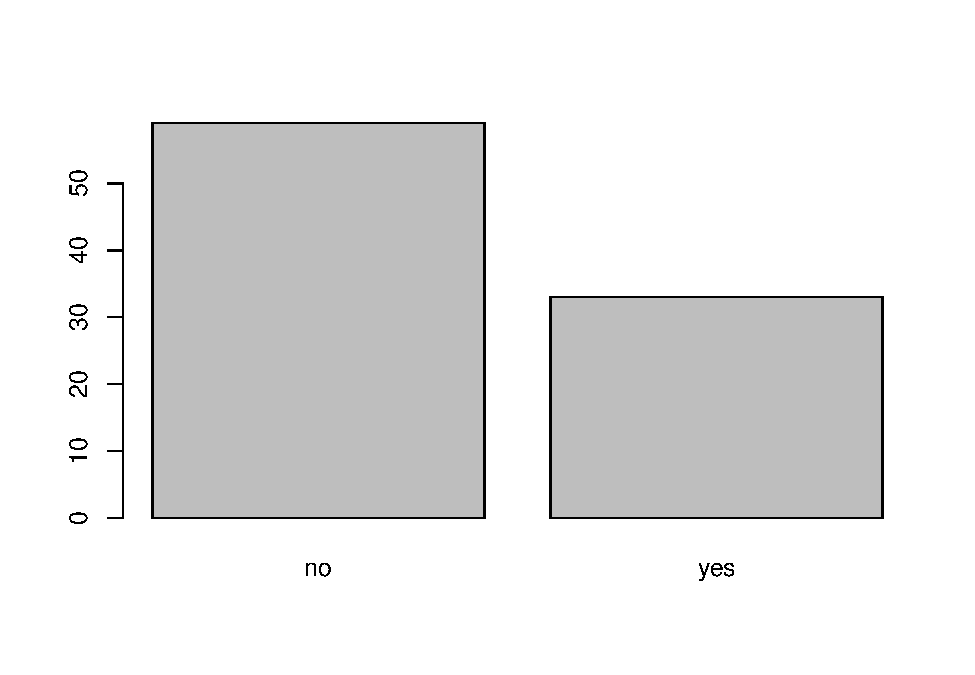
\includegraphics{2020-01-15-brynmawr_files/figure-latex/factor-plot-default-order-1.pdf}

Looking at the plot compared to the output of the vector, we can see
that n addition to ``no''s and ``yes''s, there are about some
respondents for which the information about whether they were part of an
irrigation association hasn't been recorded, and encoded as missing
data. They do not appear on the plot. Let's encode them differently so
they can counted and visualized in our plot.

\begin{Shaded}
\begin{Highlighting}[]
\NormalTok{## replace the missing data with "undetermined"}
\NormalTok{interviews <-}\StringTok{ }\NormalTok{interviews }\OperatorTok
\StringTok{  }\KeywordTok{mutate}\NormalTok{(}\DataTypeTok{memb_assoc =} \KeywordTok{fct_explicit_na}\NormalTok{(memb_assoc, }\DataTypeTok{na_level =} \StringTok{"undetermined"}\NormalTok{))}

\NormalTok{interviews}\OperatorTok{$}\NormalTok{memb_assoc}
\end{Highlighting}
\end{Shaded}

\begin{verbatim}
##   [1] undetermined yes          undetermined undetermined undetermined
##   [6] undetermined no           yes          no           no          
##  [11] undetermined yes          no           undetermined yes         
##  [16] undetermined undetermined undetermined undetermined undetermined
##  [21] no           undetermined undetermined no           no          
##  [26] no           undetermined no           yes          undetermined
##  [31] undetermined yes          no           yes          yes         
##  [36] yes          undetermined yes          undetermined yes         
##  [41] undetermined no           no           undetermined no          
##  [46] no           yes          undetermined undetermined yes         
##  [51] undetermined no           yes          no           undetermined
##  [56] yes          no           no           undetermined no          
##  [61] yes          undetermined undetermined undetermined no          
##  [66] yes          no           no           no           no          
##  [71] yes          undetermined no           yes          undetermined
##  [76] undetermined yes          no           no           yes         
##  [81] no           no           yes          no           yes         
##  [86] no           no           undetermined yes          yes         
##  [91] yes          yes          yes          no           no          
##  [96] no           no           yes          no           no          
## [101] yes          yes          no           undetermined no          
## [106] no           undetermined no           no           undetermined
## [111] no           undetermined undetermined no           no          
## [116] no           no           yes          no           no          
## [121] no           no           no           no           no          
## [126] no           no           no           no           yes         
## [131] undetermined
## Levels: yes no undetermined
\end{verbatim}

\begin{Shaded}
\begin{Highlighting}[]
\NormalTok{## bar plot of the number of interview respondents who were}
\NormalTok{## members of irrigation association:}
\KeywordTok{plot}\NormalTok{(interviews}\OperatorTok{$}\NormalTok{memb_assoc)}
\end{Highlighting}
\end{Shaded}

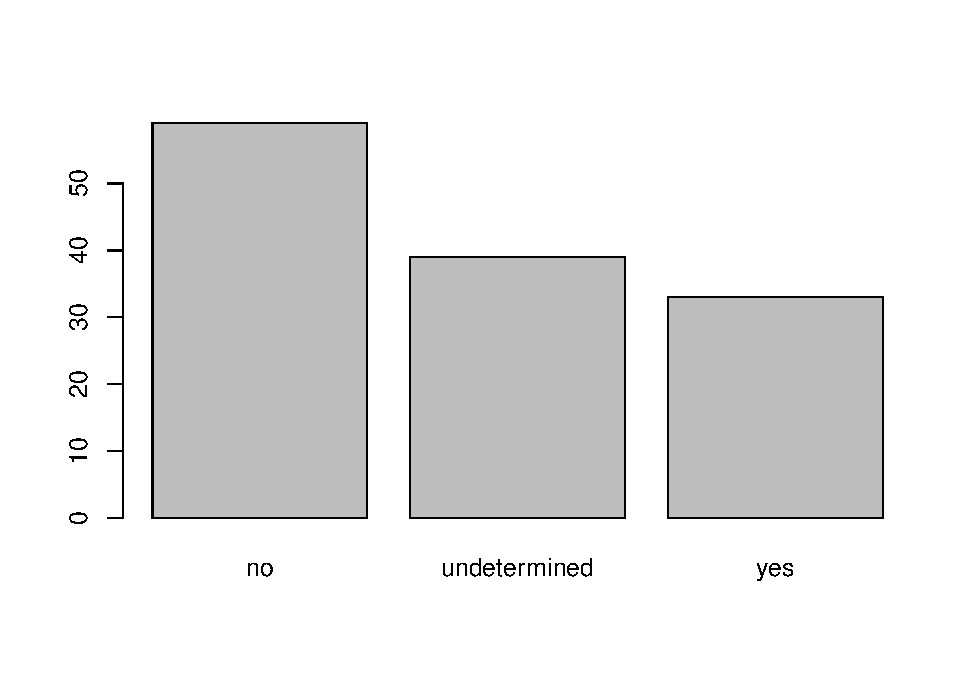
\includegraphics{2020-01-15-brynmawr_files/figure-latex/factor-plot-reorder-1.pdf}

Again, if we wanted to reorder our factor here in order of

\begin{Shaded}
\begin{Highlighting}[]
\NormalTok{interviews <-}\StringTok{ }\NormalTok{interviews }\OperatorTok
\StringTok{  }\KeywordTok{mutate}\NormalTok{(}\DataTypeTok{memb_assoc =} \KeywordTok{fct_infreq}\NormalTok{(memb_assoc, }\DataTypeTok{ordered =} \OtherTok{TRUE}\NormalTok{))}
\KeywordTok{plot}\NormalTok{(interviews}\OperatorTok{$}\NormalTok{memb_assoc)}
\end{Highlighting}
\end{Shaded}

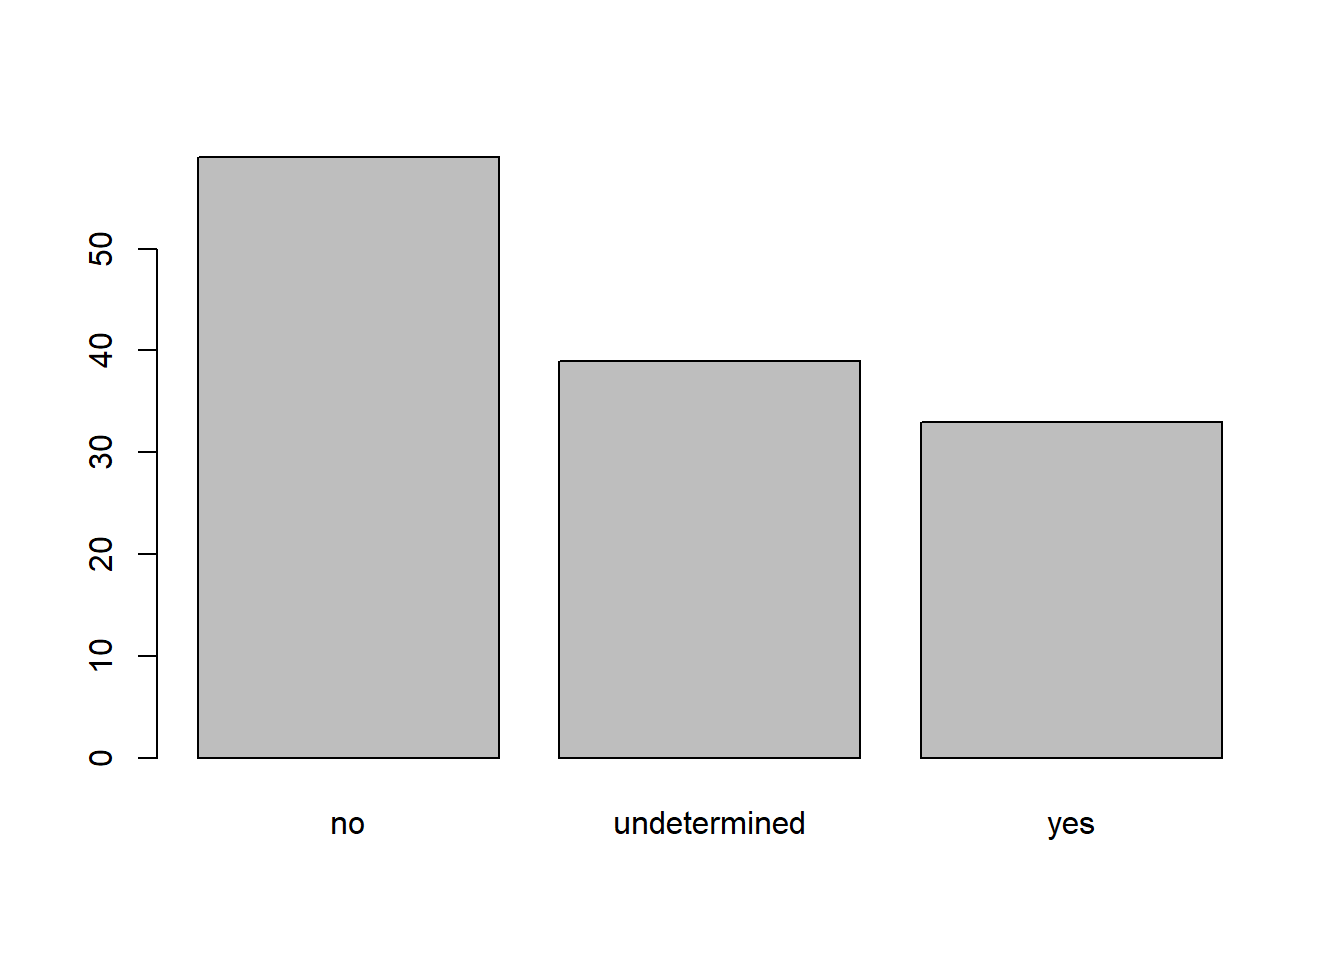
\includegraphics{2020-01-15-brynmawr_files/figure-latex/unnamed-chunk-103-1.pdf}

\begin{Shaded}
\begin{Highlighting}[]
\NormalTok{interviews <-}\StringTok{ }\NormalTok{interviews }\OperatorTok
\StringTok{  }\KeywordTok{mutate}\NormalTok{(}\DataTypeTok{memb_assoc =} \KeywordTok{fct_relevel}\NormalTok{(memb_assoc, }\StringTok{"No"}\NormalTok{, }\StringTok{"Yes"}\NormalTok{, }\StringTok{"Undetermined"}\NormalTok{))}
\end{Highlighting}
\end{Shaded}

\begin{verbatim}
## Warning: Unknown levels in `f`: No, Yes, Undetermined
\end{verbatim}

\begin{quote}
\section{Exercise}\label{exercise-16}

\begin{itemize}
\item
  Rename the levels of the factor to have the first letter in uppercase:
  ``No'',``Undetermined'', and ``Yes''.
\item
  Now that we have renamed the factor level to ``Undetermined'', can you
  recreate the barplot such that ``Undetermined'' is last (after
  ``Yes'')?
\end{itemize}

\begin{quote}
\section{Solution}\label{solution-18}

\begin{Shaded}
\begin{Highlighting}[]
\NormalTok{interviews <-}\StringTok{ }\NormalTok{interviews }\OperatorTok
\StringTok{ }\KeywordTok{mutate}\NormalTok{(}\DataTypeTok{memb_assoc =} \KeywordTok{fct_recode}\NormalTok{(memb_assoc, }\DataTypeTok{No =} \StringTok{"no"}\NormalTok{, }\DataTypeTok{Yes =} \StringTok{"yes"}\NormalTok{,}
                                \DataTypeTok{Undetermined =} \StringTok{"undetermined"}\NormalTok{))}
\KeywordTok{plot}\NormalTok{(interviews}\OperatorTok{$}\NormalTok{memb_assoc)}
\end{Highlighting}
\end{Shaded}

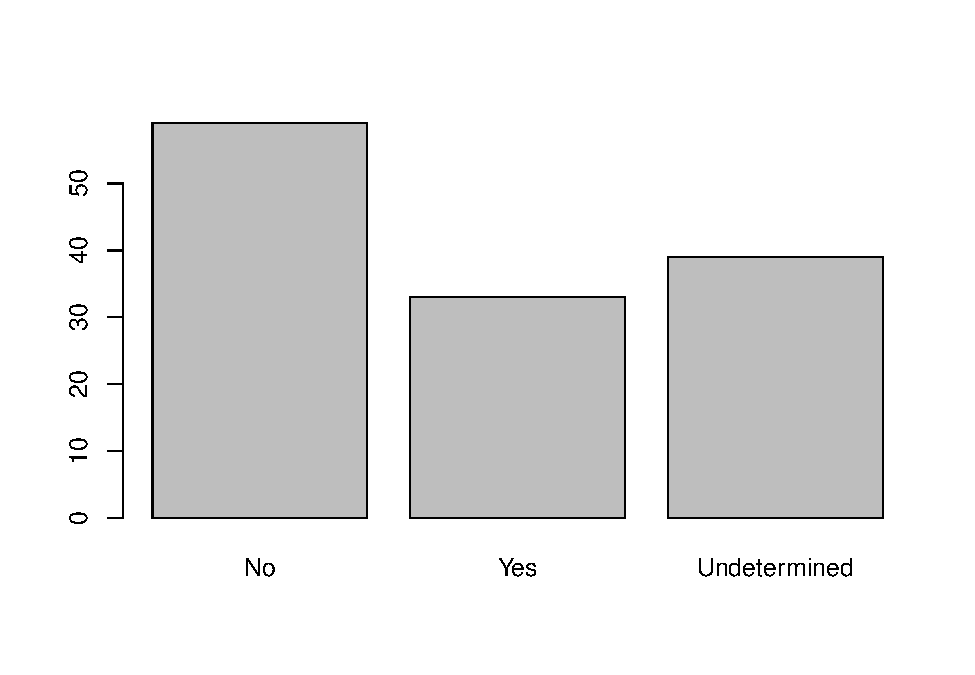
\includegraphics{2020-01-15-brynmawr_files/figure-latex/factor-plot-exercise-1.pdf}

\begin{Shaded}
\begin{Highlighting}[]
\NormalTok{interviews <-}\StringTok{ }\NormalTok{interviews }\OperatorTok
\StringTok{  }\KeywordTok{mutate}\NormalTok{(}\DataTypeTok{memb_assoc =} \KeywordTok{fct_relevel}\NormalTok{(memb_assoc, }\StringTok{"No"}\NormalTok{, }\StringTok{"Yes"}\NormalTok{, }\StringTok{"Undetermined"}\NormalTok{))}
\KeywordTok{plot}\NormalTok{(interviews}\OperatorTok{$}\NormalTok{memb_assoc)}
\end{Highlighting}
\end{Shaded}

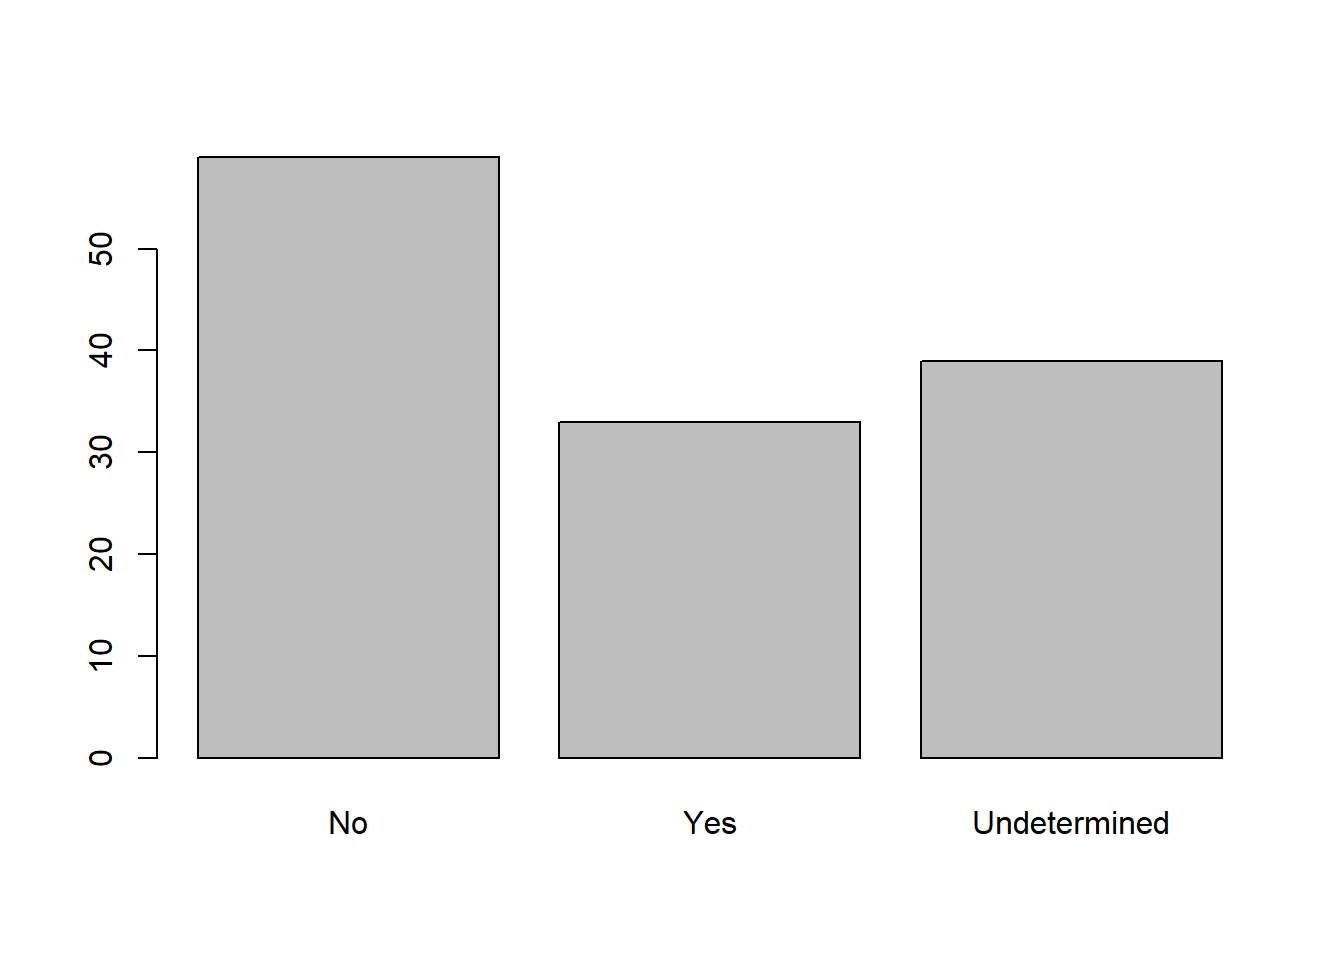
\includegraphics{2020-01-15-brynmawr_files/figure-latex/factor-plot-exercise-2.pdf}
\end{quote}
\end{quote}

\section{strings}\label{strings}

Much like \texttt{forcats} helps us deal with factor variables, there
are packages to help us deal with string variables. Some useful packages
are the \texttt{tidyr} package (which we've already seen) the
\texttt{stringr} package (installed with the tidyverse, but needs to be
loaded separately) and the \texttt{tidytext} package. Let's say we're
interested in the items owned by the interviewees. Right now, all the
items are stuck together into one not-very-useful variable,

\begin{Shaded}
\begin{Highlighting}[]
\NormalTok{interviews }\OperatorTok
\StringTok{  }\KeywordTok{select}\NormalTok{(items_owned)}
\end{Highlighting}
\end{Shaded}

\begin{verbatim}
## # A tibble: 131 x 1
##    items_owned                                                                  
##    <chr>                                                                        
##  1 bicycle;television;solar_panel;table                                         
##  2 cow_cart;bicycle;radio;cow_plough;solar_panel;solar_torch;table;mobile_phone 
##  3 solar_torch                                                                  
##  4 bicycle;radio;cow_plough;solar_panel;mobile_phone                            
##  5 motorcyle;radio;cow_plough;mobile_phone                                      
##  6 <NA>                                                                         
##  7 motorcyle;cow_plough                                                         
##  8 motorcyle;bicycle;television;radio;cow_plough;solar_panel;solar_torch;table;…
##  9 television;solar_panel;solar_torch                                           
## 10 cow_cart;motorcyle;bicycle;television;radio;cow_plough;solar_panel;solar_tor…
## # … with 121 more rows
\end{verbatim}

We'd like to know which interviewees own a bicycle, for example. One way
to do this would be to use the \texttt{stringr} package to check if a
particular string was contained in that variable,

\begin{Shaded}
\begin{Highlighting}[]
\KeywordTok{library}\NormalTok{(stringr)}
\NormalTok{interviews <-}\StringTok{ }\NormalTok{interviews }\OperatorTok
\StringTok{  }\KeywordTok{mutate}\NormalTok{(}\DataTypeTok{has_bicycle =} \KeywordTok{str_detect}\NormalTok{(items_owned, }\StringTok{"bicycle"}\NormalTok{))}

\KeywordTok{plot}\NormalTok{(}\KeywordTok{factor}\NormalTok{(interviews}\OperatorTok{$}\NormalTok{has_bicycle))}
\end{Highlighting}
\end{Shaded}

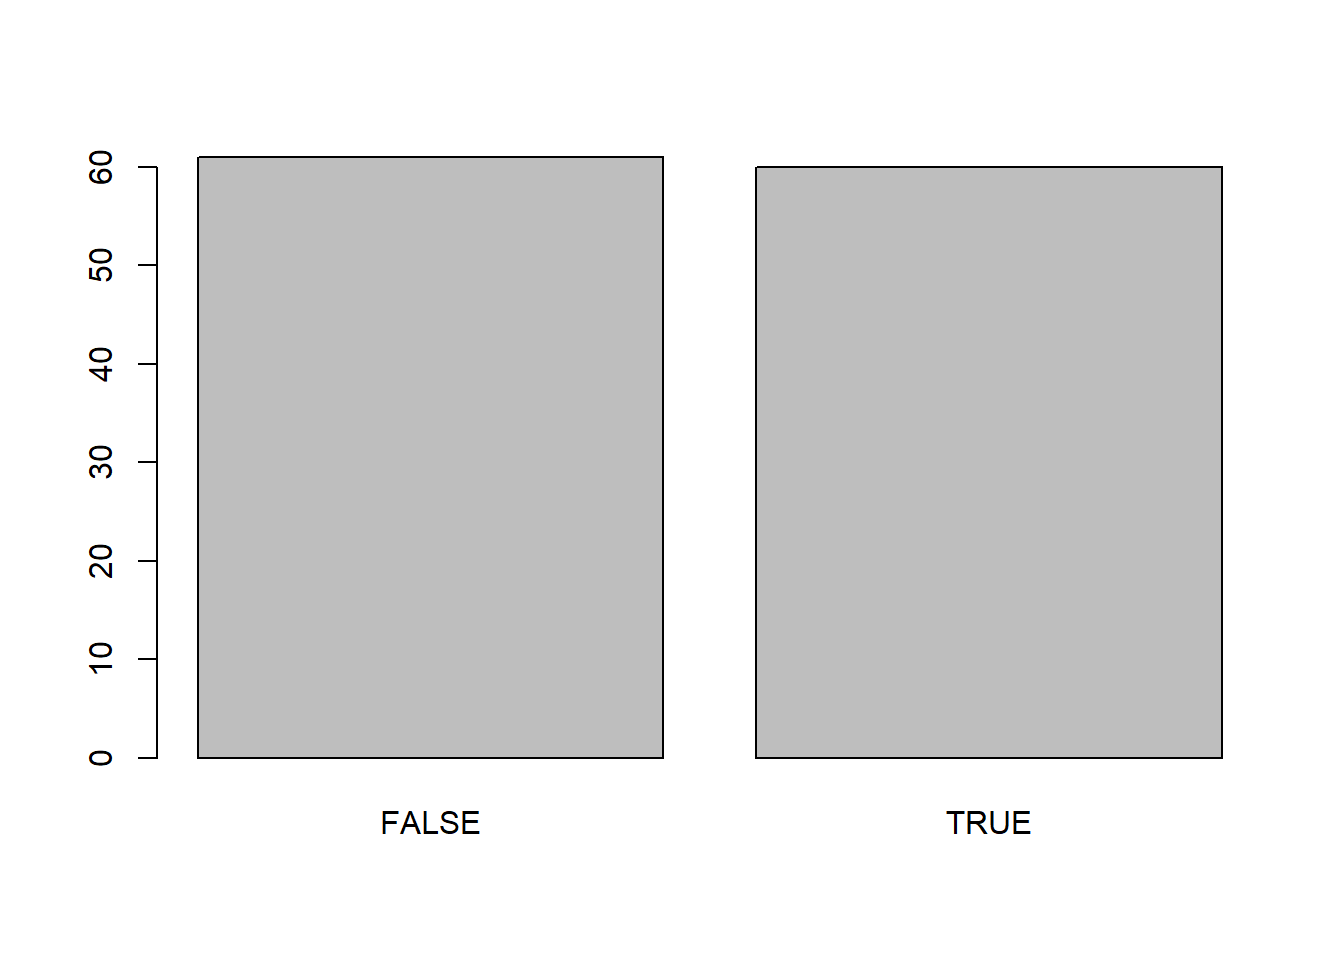
\includegraphics{2020-01-15-brynmawr_files/figure-latex/unnamed-chunk-105-1.pdf}

Much like the \texttt{forcats} package, the \texttt{stringr} package has
many functions that begin with \texttt{str\_}, so you can type that much
out and hit Tab to see other options.

We could go through manually and repeat a similar set of lines of code
for each item (\texttt{solar\_torch}, \texttt{cow\_plough}, etc) but
there is a programming principle that if you repeat yourself there is
likely a more efficient way to do it.

In this case, that more efficient solution is to use the
\texttt{tidytext} package, which lets us ``unnest'' the data into
individual words. When we start working with text in this way, it can
get a little messy, so it is often smart to break off a little piece of
your data to work with separately. Here we're taking just the
\texttt{items\_owned} variable and the \texttt{instanceID} (so we can
join this back together with our original data later, if we so choose).

\begin{Shaded}
\begin{Highlighting}[]
\NormalTok{items <-}\StringTok{ }\NormalTok{interviews }\OperatorTok
\StringTok{  }\KeywordTok{select}\NormalTok{(items_owned, instanceID)}
\end{Highlighting}
\end{Shaded}

\begin{Shaded}
\begin{Highlighting}[]
\KeywordTok{library}\NormalTok{(tidytext)}
\NormalTok{items <-}\StringTok{ }\NormalTok{items }\OperatorTok
\StringTok{  }\KeywordTok{unnest_tokens}\NormalTok{(word, items_owned)}
\end{Highlighting}
\end{Shaded}

Now we have a variable called \texttt{word}, which is all the separate
items. This is a very long dataset, so we may want to
\texttt{pivot\_wider} to make it easier to see.

\begin{Shaded}
\begin{Highlighting}[]
\NormalTok{items <-}\StringTok{ }\NormalTok{items }\OperatorTok
\StringTok{  }\KeywordTok{mutate}\NormalTok{(}\DataTypeTok{contains =} \KeywordTok{if_else}\NormalTok{(}\KeywordTok{is.na}\NormalTok{(word), }\OtherTok{FALSE}\NormalTok{, }\OtherTok{TRUE}\NormalTok{))}
\NormalTok{items <-}\StringTok{ }\NormalTok{items }\OperatorTok
\StringTok{  }\KeywordTok{pivot_wider}\NormalTok{(}\DataTypeTok{names_from =}\NormalTok{ word, }\DataTypeTok{values_from =}\NormalTok{ contains, }\DataTypeTok{values_fill =} \KeywordTok{list}\NormalTok{(}\DataTypeTok{contains =} \OtherTok{FALSE}\NormalTok{))}
\end{Highlighting}
\end{Shaded}

If we'd like, we can now use a join to stick this back to our main
dataset,

\begin{Shaded}
\begin{Highlighting}[]
\NormalTok{interviews <-}\StringTok{ }\NormalTok{interviews }\OperatorTok
\StringTok{  }\KeywordTok{left_join}\NormalTok{(items)}
\end{Highlighting}
\end{Shaded}

\begin{verbatim}
## Joining, by = "instanceID"
\end{verbatim}

Now we can see what each person owned.

\section{Formatting Dates}\label{formatting-dates}

One of the most common issues that new (and experienced!) R users have
is converting date and time information into a variable that is
appropriate and usable during analyses. As a reminder from earlier in
this lesson, the best practice for dealing with date data is to ensure
that each component of your date is stored as a separate variable. In
our dataset, we have a column \texttt{interview\_date} which contains
information about the year, month, and day that the interview was
conducted. Let's convert those dates into three separate columns.

\begin{Shaded}
\begin{Highlighting}[]
\KeywordTok{str}\NormalTok{(interviews)}
\end{Highlighting}
\end{Shaded}

We are going to use the package \textbf{\texttt{lubridate}} (which
belongs to the \textbf{\texttt{tidyverse}}; learn more
\href{https://www.tidyverse.org/}{here}) to work with dates.
\textbf{\texttt{lubridate}} gets installed as part as the
\textbf{\texttt{tidyverse}} installation. When you load the
\textbf{\texttt{tidyverse}} (\texttt{library(tidyverse)}), the core
packages (the packages used in most data analyses) get loaded.
\textbf{\texttt{lubridate}} however does not belong to the core
tidyverse, so you have to load it explicitly with
\texttt{library(lubridate)}

Start by loading the required package:

\begin{Shaded}
\begin{Highlighting}[]
\KeywordTok{library}\NormalTok{(lubridate)}
\end{Highlighting}
\end{Shaded}

The lubridate function \texttt{ymd()} takes a vector representing year,
month, and day, and converts it to a \texttt{Date} vector. \texttt{Date}
is a class of data recognized by R as being a date and can be
manipulated as such. The argument that the function requires is
flexible, but, as a best practice, is a character vector formatted as
``YYYY-MM-DD''.

Let's extract our \texttt{interview\_date} column and inspect the
structure:

\begin{Shaded}
\begin{Highlighting}[]
\NormalTok{dates <-}\StringTok{ }\NormalTok{interviews}\OperatorTok{$}\NormalTok{interview_date}
\KeywordTok{str}\NormalTok{(dates)}
\end{Highlighting}
\end{Shaded}

\begin{verbatim}
##  POSIXct[1:131], format: "2016-11-17" "2016-11-17" "2016-11-17" "2016-11-17" "2016-11-17" ...
\end{verbatim}

When we imported the data in R, \texttt{read\_csv()} recognized that
this column contained date information. We can now use the
\texttt{day()}, \texttt{month()} and \texttt{year()} functions to
extract this information from the date, and create new columns in our
data frame to store it:

\begin{Shaded}
\begin{Highlighting}[]
\NormalTok{interviews}\OperatorTok{$}\NormalTok{day <-}\StringTok{ }\KeywordTok{day}\NormalTok{(dates)}
\NormalTok{interviews}\OperatorTok{$}\NormalTok{month <-}\StringTok{ }\KeywordTok{month}\NormalTok{(dates)}
\NormalTok{interviews}\OperatorTok{$}\NormalTok{year <-}\StringTok{ }\KeywordTok{year}\NormalTok{(dates)}
\NormalTok{interviews}
\end{Highlighting}
\end{Shaded}

\begin{verbatim}
## # A tibble: 131 x 36
##    key_ID village interview_date      no_membrs years_liv respondent_wall… rooms
##     <dbl> <chr>   <dttm>                  <dbl>     <dbl> <chr>            <dbl>
##  1      1 God     2016-11-17 00:00:00         3         4 muddaub              1
##  2      1 God     2016-11-17 00:00:00         7         9 muddaub              1
##  3      3 God     2016-11-17 00:00:00        10        15 burntbricks          1
##  4      4 God     2016-11-17 00:00:00         7         6 burntbricks          1
##  5      5 God     2016-11-17 00:00:00         7        40 burntbricks          1
##  6      6 God     2016-11-17 00:00:00         3         3 muddaub              1
##  7      7 God     2016-11-17 00:00:00         6        38 muddaub              1
##  8      8 Chirod… 2016-11-16 00:00:00        12        70 burntbricks          3
##  9      9 Chirod… 2016-11-16 00:00:00         8         6 burntbricks          1
## 10     10 Chirod… 2016-12-16 00:00:00        12        23 burntbricks          5
## # … with 121 more rows, and 29 more variables: memb_assoc <ord>,
## #   affect_conflicts <chr>, liv_count <dbl>, items_owned <chr>, no_meals <dbl>,
## #   months_lack_food <chr>, instanceID <chr>, has_bicycle <lgl>, bicycle <lgl>,
## #   television <lgl>, solar_panel <lgl>, table <lgl>, cow_cart <lgl>,
## #   radio <lgl>, cow_plough <lgl>, solar_torch <lgl>, mobile_phone <lgl>,
## #   motorcyle <lgl>, `NA` <lgl>, fridge <lgl>, electricity <lgl>,
## #   sofa_set <lgl>, lorry <lgl>, sterio <lgl>, computer <lgl>, car <lgl>,
## #   day <int>, month <dbl>, year <dbl>
\end{verbatim}

Notice the three new columns at the end of our data frame.

\chapter{\texorpdfstring{Producing Reports With
\texttt{knitr}}{Producing Reports With knitr}}\label{knitr}

teaching: 60\\
exercises: 15\\
adapted from:
\url{http://swcarpentry.github.io/r-novice-gapminder/15-knitr-markdown/index.html}\\
questions:

\begin{itemize}
\tightlist
\item
  ``How can I integrate software and reports?''
\end{itemize}

objectives:

\begin{itemize}
\tightlist
\item
  Understand the value of writing reproducible reports\\
\item
  Learn how to recognise and compile the basic components of an R
  Markdown file\\
\item
  Become familiar with R code chunks, and understand their purpose,
  structure and options\\
\item
  Demonstrate the use of inline chunks for weaving R outputs into text
  blocks, for example when discussing the results of some calculations\\
\item
  Be aware of alternative output formats to which an R Markdown file can
  be exported
\end{itemize}

keypoints:

\begin{itemize}
\tightlist
\item
  ``Mix reporting written in R Markdown with software written in R.''\\
\item
  ``Specify chunk options to control formatting.''\\
\item
  ``Use \texttt{knitr} to convert these documents into PDF and other
  formats.''
\end{itemize}

\section{Data analysis reports}\label{data-analysis-reports}

Data analysts tend to write a lot of reports, describing their analyses
and results, for their collaborators or to document their work for
future reference.

Many new users begin by first writing a single R script containing all
of the work. Then simply share the analysis by emailing the script and
various graphs as attachments. But this can be cumbersome, requiring a
lengthy discussion to explain which attachment was which result.

Writing formal reports with Word or
\href{http://www.latex-project.org/}{LaTeX} can simplify this by
incorporating both the analysis report and output graphs into a single
document. But tweaking formatting to make figures look correct and fix
obnoxious page breaks can be tedious and lead to a lengthly ``whack a
mole'' game of fixing new mistakes resulting from a single formatting
change.

Creating a web page (as an html file) by using R Markdown makes things
easier. The report can be one long stream, so tall figures that wouldn't
ordinary fit on one page can be kept full size and easier to read, since
the reader can simply keep scrolling. Formatting is simple and easy to
modify, allowing you to spend more time on your analyses instead of
writing reports.

\section{Literate programming}\label{literate-programming}

Ideally, such analysis reports are \emph{reproducible} documents: If an
error is discovered, or if some additional subjects are added to the
data, you can just re-compile the report and get the new or corrected
results (versus having to reconstruct figures, paste them into a Word
document, and further hand-edit various detailed results).

The key R package is \href{http://yihui.name/knitr/}{\texttt{knitr}}. It
allows you to create a document that is a mixture of text and chunks of
code. When the document is processed by \texttt{knitr}, chunks of code
will be executed, and graphs or other results inserted into the final
document.

This sort of idea has been called ``literate programming''.

\texttt{knitr} allows you to mix basically any sort of text with code
from different programming languages, but we recommend that you use
\texttt{R\ Markdown}, which mixes Markdown with R.
\href{https://www.markdownguide.org/}{Markdown} is a light-weight
mark-up language for creating web pages.

\section{Markdown}\label{markdown}

Markdown is a system for writing web pages by marking up the text much
as you would in an email rather than writing html code. The marked-up
text gets \emph{converted} to html, replacing the marks with the proper
html code.

For now, let's delete all of the stuff that's there and write a bit of
markdown.

You make things \textbf{bold} using two asterisks, like this:
\texttt{**bold**}, and you make things \emph{italics} by using
underscores, like this: \texttt{\_italics\_}.

You can make a bulleted list by writing a list with hyphens or
asterisks, like this:

\begin{verbatim}
* bold with double-asterisks
* italics with underscores
* code-type font with backticks
\end{verbatim}

or like this:

\begin{verbatim}
- bold with double-asterisks
- italics with underscores
- code-type font with backticks
\end{verbatim}

Each will appear as:

\begin{itemize}
\tightlist
\item
  bold with double-asterisks
\item
  italics with underscores
\item
  code-type font with backticks
\end{itemize}

You can use whatever method you prefer, but \emph{be consistent}. This
maintains the readability of your code.

You can make a numbered list by just using numbers. You can even use the
same number over and over if you want:

\begin{verbatim}
1. bold with double-asterisks
1. italics with underscores
1. code-type font with backticks
\end{verbatim}

This will appear as:

\begin{enumerate}
\def\labelenumi{\arabic{enumi}.}
\tightlist
\item
  bold with double-asterisks
\item
  italics with underscores
\item
  code-type font with backticks
\end{enumerate}

You can make section headers of different sizes by initiating a line
with some number of \texttt{\#} symbols:

\begin{verbatim}
# Title
## Main section
### Sub-section
#### Sub-sub section
\end{verbatim}

You \emph{compile} the R Markdown document to an html webpage by
clicking the ``Knit'' button in the upper-left.

\begin{quote}
\section{Challenge 1}\label{challenge-1-1}

Create a new R Markdown document. Delete all of the R code chunks and
write a bit of Markdown (some sections, some italicized text, and an
itemized list).

Convert the document to a webpage. \textgreater{} \#\# Solution to
Challenge 1 \textgreater{} \textgreater{} In RStudio, select File
\textgreater{} New file \textgreater{} R Markdown\ldots{} \textgreater{}
\textgreater{} Delete the placeholder text and add the following:
\textgreater{} \textgreater{}
\texttt{\textgreater{}\ \#\ Introduction\ \textgreater{}\ \textgreater{}\ \#\#\ Background\ on\ Data\ \textgreater{}\ \textgreater{}\ This\ report\ uses\ the\ *SAFI*\ dataset,\ which\ has\ columns\ that\ include:\ \textgreater{}\ \textgreater{}\ *\ country\ \textgreater{}\ *\ continent\ \textgreater{}\ *\ year\ \textgreater{}\ *\ lifeExp\ \textgreater{}\ *\ pop\ \textgreater{}\ *\ gdpPercap\ \textgreater{}\ \textgreater{}\ \#\#\ Background\ on\ Methods\ \textgreater{}\ \textgreater{}}
\textgreater{} \textgreater{} Then click the `Knit' button on the
toolbar to generate an html document (webpage).
\end{quote}

\section{A bit more Markdown}\label{a-bit-more-markdown}

You can make a hyperlink like this:
\texttt{{[}text\ to\ show{]}(http://the-web-page.com)}.

You can include an image file like this:
\texttt{!{[}caption{]}(http://url/for/file)}

You can do subscripts (e.g., F\textsubscript{2}) with
\texttt{F\textasciitilde{}2\textasciitilde{}} and superscripts (e.g.,
F\textsuperscript{2}) with \texttt{F\^{}2\^{}}.

If you know how to write equations in
\href{http://www.latex-project.org/}{LaTeX}, you can use \texttt{\$\ \$}
and \texttt{\$\$\ \$\$} to insert math equations, like
\texttt{\$E\ =\ mc\^{}2\$} and

\begin{verbatim}
$$y = \mu + \sum_{i=1}^p \beta_i x_i + \epsilon$$
\end{verbatim}

You can review Markdown syntax by navigating to the ``Markdown Quick
Reference'' under the ``Help'' field in the toolbar at the top of
RStudio.

\section{R code chunks}\label{r-code-chunks}

The real power of Markdown comes from mixing markdown with chunks of
code. This is R Markdown. When processed, the R code will be executed;
if they produce figures, the figures will be inserted in the final
document.

The main code chunks look like this:

That is, you place a chunk of R code between ```\{r chunk\_name\} and
```. You should give each chunk a unique name, as they will help you to
fix errors and, if any graphs are produced, the file names are based on
the name of the code chunk that produced them.

\begin{quote}
\section{Challenge 2}\label{challenge-2-1}

Add code chunks to:

\begin{itemize}
\tightlist
\item
  Load the ggplot2 package
\item
  Read the gapminder data
\item
  Create a plot
\end{itemize}

\begin{quote}
\section{Solution to Challenge 2}\label{solution-to-challenge-2-1}
\end{quote}
\end{quote}

\section{How things get compiled}\label{how-things-get-compiled}

When you press the ``Knit'' button, the R Markdown document is processed
by \href{http://yihui.name/knitr}{\texttt{knitr}} and a plain Markdown
document is produced (as well as, potentially, a set of figure files):
the R code is executed and replaced by both the input and the output; if
figures are produced, links to those figures are included.

The Markdown and figure documents are then processed by the tool
\href{http://pandoc.org/}{\texttt{pandoc}}, which converts the Markdown
file into an html file, with the figures embedded.

\begin{flushleft}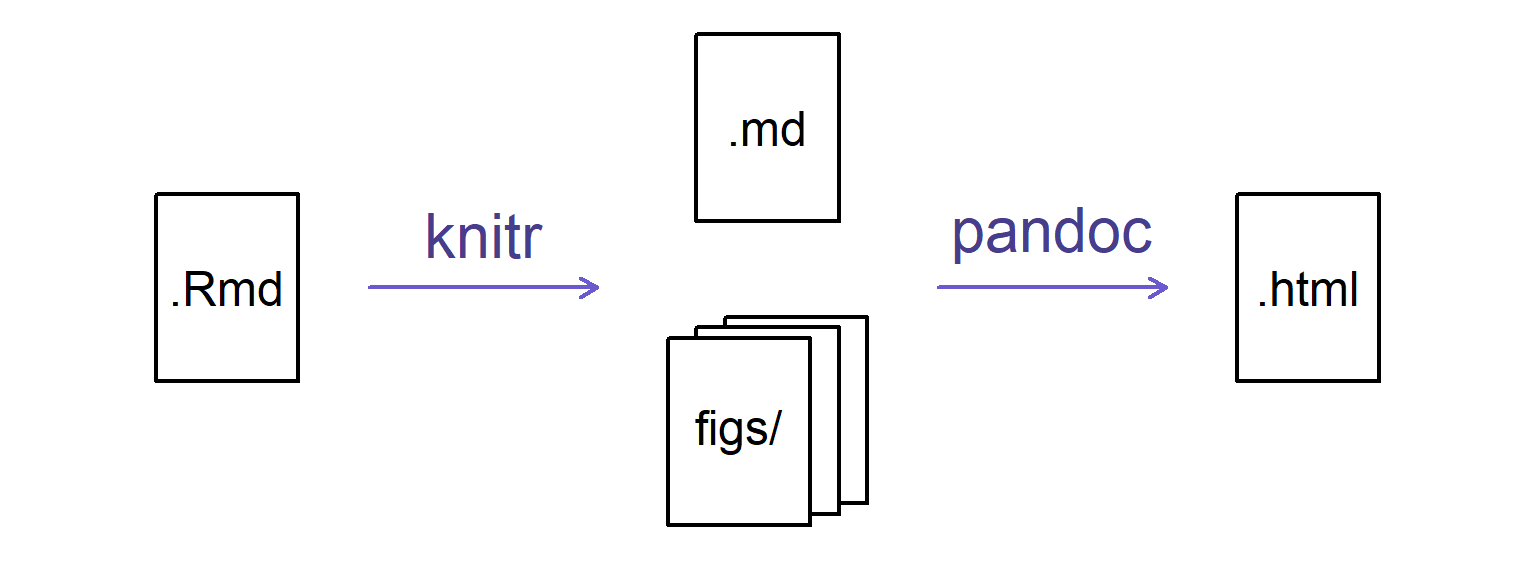
\includegraphics{2020-01-15-brynmawr_files/figure-latex/rmd_to_html_fig-1} \end{flushleft}

\section{Chunk options}\label{chunk-options}

There are a variety of options to affect how the code chunks are
treated. Here are some examples:

\begin{itemize}
\tightlist
\item
  Use \texttt{echo=FALSE} to avoid having the code itself shown.
\item
  Use \texttt{results="hide"} to avoid having any results printed.
\item
  Use \texttt{eval=FALSE} to have the code shown but not evaluated.
\item
  Use \texttt{warning=FALSE} and \texttt{message=FALSE} to hide any
  warnings or messages produced.
\item
  Use \texttt{fig.height} and \texttt{fig.width} to control the size of
  the figures produced (in inches).
\end{itemize}

So you might write:

Often there will be particular options that you'll want to use
repeatedly; for this, you can set \emph{global} chunk options, like so:

The \texttt{fig.path} option defines where the figures will be saved.
The \texttt{/} here is really important; without it, the figures would
be saved in the standard place but just with names that begin with
\texttt{Figs}.

If you have multiple R Markdown files in a common directory, you might
want to use \texttt{fig.path} to define separate prefixes for the figure
file names, like \texttt{fig.path="Figs/cleaning-"} and
\texttt{fig.path="Figs/analysis-"}.

\begin{quote}
\section{Challenge 3}\label{challenge-3-1}

Use chunk options to control the size of a figure and to hide the code.

\begin{quote}
\section{Solution to Challenge 3}\label{solution-to-challenge-3}
\end{quote}
\end{quote}

You can review all of the \texttt{R} chunk options by navigating to the
``R Markdown Cheat Sheet'' under the ``Cheatsheets'' section of the
``Help'' field in the toolbar at the top of RStudio.

\section{Inline R code}\label{inline-r-code}

You can make \emph{every} number in your report reproducible. Use `r and
` for an in-line code chunk, like so: `r round(some\_value, 2)`. The
code will be executed and replaced with the \emph{value} of the result.

Don't let these in-line chunks get split across lines.

Perhaps precede the paragraph with a larger code chunk that does
calculations and defines variables, with \texttt{include=FALSE} for that
larger chunk (which is the same as \texttt{echo=FALSE} and
\texttt{results="hide"}).

Rounding can produce differences in output in such situations. You may
want \texttt{2.0}, but \texttt{round(2.03,\ 1)} will give just
\texttt{2}.

The
\href{https://github.com/kbroman/broman/blob/master/R/myround.R}{\texttt{myround}}
function in the \href{https://github.com/kbroman/broman}{R/broman}
package handles this.

\begin{quote}
\section{Challenge 4}\label{challenge-4}

Try out a bit of in-line R code.

\begin{quote}
\section{Solution to Challenge 4}\label{solution-to-challenge-4}

Here's some inline code to determine that 2 + 2 =
\texttt{\textasciigrave{}r\ 2+2\textasciigrave{}}.
\end{quote}
\end{quote}

\section{Other output options}\label{other-output-options}

You can also convert R Markdown to a PDF or a Word document. Click the
little triangle next to the ``Knit'' button to get a drop-down menu. Or
you could put \texttt{pdf\_document} or \texttt{word\_document} in the
initial header of the file.

\begin{quote}
\section{Tip: Creating PDF documents}\label{tip-creating-pdf-documents}

Creating .pdf documents may require installation of some extra software.
If required this is detailed in an error message.

\begin{itemize}
\tightlist
\item
  \href{https://miktex.org/2.9/setup}{TeX installers for Windows}.
\item
  \href{https://tug.org/mactex}{TeX installers for macOS}.
\end{itemize}
\end{quote}

\section{Resources}\label{resources}

\begin{itemize}
\tightlist
\item
  \href{http://kbroman.org/knitr_knutshell}{Knitr in a knutshell
  tutorial}
\item
  \href{http://www.amazon.com/exec/obidos/ASIN/1482203537/7210-20}{Dynamic
  Documents with R and knitr} (book)
\item
  \href{http://rmarkdown.rstudio.com}{R Markdown documentation}
\item
  \href{https://www.rstudio.com/wp-content/uploads/2016/03/rmarkdown-cheatsheet-2.0.pdf}{R
  Markdown cheat sheet}
\item
  \href{https://www.rstudio.com/resources/webinars/getting-started-with-r-markdown/}{Getting
  started with R Markdown}
\item
  \href{https://bookdown.org/yihui/rmarkdown/}{R Markdown: The
  Definitive Guide} (book by Rstudio team)
\item
  \href{https://www.rstudio.com/resources/webinars/reproducible-reporting/}{Reproducible
  Reporting}
\item
  \href{https://www.rstudio.com/resources/webinars/the-ecosystem-of-r-markdown/}{The
  Ecosystem of R Markdown}
\item
  \href{https://www.rstudio.com/resources/webinars/introducing-bookdown/}{Introducing
  Bookdown}
\end{itemize}

\bibliography{book.bib,packages.bib}

\end{document}
